\documentclass{book}
\usepackage{a4wide}

%% possible fonts -- in order of preference
%%\usepackage{palatino}
\usepackage{bookman}
%%\usepackage{charter}
%%\usepackage{newcent}
%%\usepackage{times}
%%\usepackage{avant}
%%\usepackage{helvet}
%%\usepackage{sans}
%%\usepackage{chancery}

\usepackage[svgnames]{xcolor}	% for color text support
\usepackage[T1]{fontenc}
\usepackage[11pt]{moresize}
\usepackage{setspace}
\usepackage{ifpdf}
\usepackage{makeidx}
\usepackage{longtable}  %% page wrapping table environment
\usepackage{colortbl}   %% colors for tables
\usepackage{fancyvrb}   %% the "Verbatim" environment
\usepackage{fancyhdr}   %% custom headers and footers
\usepackage{multicol}
\usepackage{listings}   %% source code listings with syntax highlight (lstxxx commands)
\usepackage[tight]{shorttoc}   %% for generating a second table of contents, only containing chapter titles
\usepackage{bytefield}  %% for drawing protocol frames
\usepackage{paralist}   %% for compact lists
\usepackage[nottoc]{tocbibind}  %% makes Bibliography and Index show up in TOC
\settocbibname{References}

\setlength{\textwidth}{160mm}
%\setlength{\oddsidemargin}{12.5mm}
%\setlength{\evensidemargin}{12.5mm}
%\setlength{\topmargin}{0mm}
\setlength{\textheight}{220mm}
%\setlength{\parskip}{1ex}
%\setlength{\parindent}{5ex}

\renewcommand{\bottomfraction}{0.9}
\renewcommand{\topfraction}{0.9}
\renewcommand{\floatpagefraction}{0.9}

\newenvironment{htmlonly}{\expandafter\comment}{\expandafter\endcomment}
\newcommand{\pdfonly}{}

%% try to cure overfull hboxes
%% \tolerance=500

%% for navigation in dvi files, only needed by old teTeX versions
%%\usepackage{srcltx}

%% try this for spell checking: cat ess2002.tex | ispell -l -t -a | sort | uniq | more

%%
%% The following snippet changes the horizontal spacing between the number and
%% the title in the table of contents.
%%
%% http://tex.stackexchange.com/questions/33841/how-to-modify-the-space-between-the-numbers-and-text-of-sectioning-titles-in-the
%%
\makeatletter
 \renewcommand*\l@section{\@dottedtocline{1}{2em}{3em}}
 \renewcommand*\l@subsection{\@dottedtocline{2}{5em}{4em}}
\renewcommand*\l@chapter[2]{%
  \ifnum \c@tocdepth >\m@ne
    \addpenalty{-\@highpenalty}%
    \vskip 1.0em \@plus\p@
    \setlength\@tempdima{2em}%
    \begingroup
      \parindent \z@ \rightskip \@pnumwidth
      \parfillskip -\@pnumwidth
      \leavevmode \bfseries
      \advance\leftskip\@tempdima
      \hskip -\leftskip
      #1\nobreak\hfil \nobreak\hb@xt@\@pnumwidth{\hss #2}\par
      \penalty\@highpenalty
    \endgroup
  \fi}
\makeatother

%%
%% OMNeT++ logo, use as {\opp}
%%
\makeatletter
%%\DeclareRobustCommand{\omnetpp}{OM\-NeT\kern-.18em++\@}
\DeclareRobustCommand{\omnetpp}{OMNeT++\@}
\makeatother

\newcommand{\opp}{\omnetpp}

%%
%% PDF Header
%%
% note: \ifpdf now comes from the ifpdf package
%\newif\ifpdf
%\ifx\pdfoutput\undefined
%  \pdffalse
%\else
%  \pdfoutput=1
%  \pdftrue
%\fi
%% PDF-Info
\ifpdf
  \usepackage[pdftex]{graphicx}
  \usepackage[plainpages=false,linktocpage,bookmarksnumbered=true,pdftex]{hyperref}   %% automatic hyperlinking
  \pdfcompresslevel=9
  \pdfinfo{/Author (Andras Varga and others)
    /Title (INET Framework Developer's Guide)
    /Subject ()
    /Keywords (INET, INETMANET, OMNeT++, manual)}
\else
  \usepackage{graphicx}
  \usepackage[plainpages=false]{hyperref}   %% automatic hyperlinking
\fi

%%
%% Draft conditional to include unfinished parts
%%
\newif\ifdraft
\draftfalse %% uncomment for final version
%\drafttrue %% uncomment for draft version

%%
%% Generate Index
%%
\makeindex


%%
%% Link colors (hyperref package)
%%
\definecolor{MyDarkBlue}{rgb}{0.16,0.16,0.5}
%% XXX the next line apparently screws up all links except in TOC! they'll be colored nicely, but won't work.
%\hypersetup{
%    colorlinks=true,
%    linkcolor=MyDarkBlue,
%    anchorcolor=MyDarkBlue,
%    citecolor=MyDarkBlue,
%    filecolor=MyDarkBlue,
%    menucolor=MyDarkBlue,
%    runcolor=MyDarkBlue,
%    urlcolor=blue,
%}

%%
%% Heading and Footer
%%
\pagestyle{fancy}
\fancyhf{}
\renewcommand{\footrulewidth}{0.5pt}
\renewcommand{\chaptermark}[1]{\markboth{#1}{}}
\lhead{INET Framework Developer's Guide -- \leftmark}
\rfoot{\thepage}

%% this is used for chapter start pages
\fancypagestyle{plain}{
    \rfoot{\thepage}
}

%%
%% Use \begin{graybox}...\end{graybox} for notes
%%
\definecolor{MyGray}{rgb}{0.85,0.85,1.0}
\makeatletter\newenvironment{graybox}%
   {\begin{flushright}\begin{lrbox}{\@tempboxa}\begin{minipage}[r]{0.95\textwidth}}%
   {\end{minipage}\end{lrbox}\colorbox{MyGray}{\usebox{\@tempboxa}}\end{flushright}}%
\makeatother


\newenvironment{note}{\begin{graybox}\textbf{NOTE: }}{\end{graybox}}
\newenvironment{warning}{\begin{graybox}\textbf{WARNING: }}{\end{graybox}}
\newenvironment{caution}{\begin{graybox}\textbf{CAUTION: }}{\end{graybox}}
\newenvironment{rationale}{\begin{graybox}\textbf{Rationale: }}{\end{graybox}}
\newenvironment{important}{\begin{graybox}\textbf{IMPORTANT: }}{\end{graybox}}

%%
%% Set up listings package
%%
\lstloadlanguages{C++,make,perl,tcl,XML,R,Matlab}

%% See listings.pdf,pp20
\lstdefinelanguage{NED} {
    morekeywords={allowunconnected,bool,channel,channelinterface,connections,const,
                  default,double,extends,false,for,gates,if,import,index,inout,input,
                  int,like,module,moduleinterface,network,output,package,parameters,
                  property,simple,sizeof,string,submodules,this,true,types,volatile,
                  xml,xmldoc},
    sensitive=true,
    morecomment=[l]{//},
    morestring=[b]",
}
\lstdefinelanguage{MSG} {
    morekeywords={abstract,bool,char,class,cplusplus,double,enum,extends,false,
                  fields,int,long,message,namespace,noncobject,packet,properties,
                  readonly,short,string,struct,true,unsigned},
    sensitive=true,
    morecomment=[l]{//},
    morestring=[b]",
}
\lstdefinelanguage{inifile} {
    morekeywords={},
    sensitive=true,
    morecomment=[l]{\#},
    morestring=[b]",
}
\lstdefinelanguage{pseudocode} {
    morekeywords={if,then,else,otherwise,whenever,while},
    sensitive=true,
    morecomment=[l]{//},
    morestring=[b]",
    mathescape=true,
}

%% thick ruler on the left; also, designate backtick as LaTeX escape character
%% (e.g. \opp needs to be written as `\opp` inside listing blocks)
\lstset{
    escapechar=`,
    basicstyle=\ttfamily,
    identifierstyle=\color{Black},
    stringstyle=\color{DarkBlue},
    commentstyle=\color{SeaGreen},
    keywordstyle=\bfseries\color{Purple},
    showstringspaces=false,
    frame=leftline,
    framesep=10pt,
    framerule=3pt,
    xleftmargin=15pt
}

\definecolor{NEDRulerColor}{rgb}{0.5,1.0,0.5}  % pale green
\definecolor{MSGRulerColor}{rgb}{0.5,1.0,0.5}  % pale green
\definecolor{CPPRulerColor}{rgb}{0.8,0.5,0.2}  % pale orange
\definecolor{IniRulerColor}{rgb}{0.9,0.9,0.3}  % pale yellow
\definecolor{FileListingRulerColor}{rgb}{0.85,0.85,0.85}  % grey
%\definecolor{CommandLineRulerColor}{rgb}{0.9,0.9,0.2}
\definecolor{PseudoCodeRulerColor}{rgb}{0.0,1.0,1.0}  % cyan
\definecolor{XMLRulerColor}{rgb}{0.8,0.8,1.0}  % pale blue

%% See listings.pdf,pp39
\lstnewenvironment{ned}
    {\lstset{language=NED,rulecolor=\color{NEDRulerColor}}}
    {}
\lstnewenvironment{msg}
    {\lstset{language=MSG,rulecolor=\color{MSGRulerColor}}}
    {}
\lstnewenvironment{cpp}
    {\lstset{language=C++,rulecolor=\color{CPPRulerColor}}}
    {}
\lstnewenvironment{inifile}
    {\lstset{language=inifile,rulecolor=\color{IniRulerColor}}}
    {}
\lstnewenvironment{filelisting}
    {\lstset{language={},rulecolor=\color{FileListingRulerColor}}}
    {}
\lstnewenvironment{commandline}
    {\lstset{language={},framesep=11pt,framerule=1pt,xleftmargin=16pt}}
    {}
\lstnewenvironment{pseudocode}
    {\lstset{language=pseudocode,rulecolor=\color{PseudoCodeRulerColor}}}
    {}
\lstnewenvironment{XML}
    {\lstset{language=XML,rulecolor=\color{XMLRulerColor}}}
    {}

% add caption={#2} to display caption
\newcommand{\xmlsnippet}[2]{%
    \lstinputlisting[language=XML,rulecolor=\color{XMLRulerColor},linerange=<!\-\-#1\-\->-<!\-\-End\-\->,includerangemarker=false,firstnumber=0]{lib/Snippets.xml}}
\newcommand{\cppsnippet}[2]{%
    \lstinputlisting[language=C++,rulecolor=\color{CPPRulerColor},linerange=//!#1-//!End,includerangemarker=false,firstnumber=0]{lib/Snippets.cc}}
\newcommand{\msgsnippet}[2]{%
    \lstinputlisting[language=msg,rulecolor=\color{MSGRulerColor},linerange=//!#1-//!End,includerangemarker=false,firstnumber=0]{lib/Snippets.msg}}
\newcommand{\nedsnippet}[2]{%
    \lstinputlisting[language=ned,rulecolor=\color{NEDRulerColor},linerange=//!#1-//!End,includerangemarker=false,firstnumber=0]{lib/Snippets.ned}}
\newcommand{\inisnippet}[2]{%
    \lstinputlisting[language=inifile,rulecolor=\color{IniRulerColor},linerange=\#!#1-\#!End,includerangemarker=false,firstnumber=0]{lib/Snippets.ini}}

%%
%% some customization
%%
\setlength{\parindent}{0pt}
\setlength{\parskip}{1ex}

%%
%% Shortcuts
%%
\newcommand{\appendixchapter}{\chapter} %% html converter needs to know which chapters are appendices

\newcommand{\tbf}{\textbf} %% bold faced text
\newcommand{\ttt}{\texttt} %% type writer font text

\newcommand{\tab}{\hspace*{5mm}} %% tabulator settings

\newcommand{\new}{$^{New!}$}
\newcommand{\changed}{$^{Changed!}$}

%% Colordefinition for table header rows (requires package colortbl)
\newcommand{\tabheadcol}{\rowcolor[gray]{0.8}}

%%
%% Module parameters list
%%
\newenvironment{params}{\begin{itemize}}{\end{itemize}}
\newcommand{\param}[2]{\item \fpar{#1}: #2}

%%
%% Function/Class/Macro/Variable/Program/Parameter/Define names
%%
%% Write the names in type writer font and do an index entry
%% Allows word wrap by automatic hyphenation
%%
%% Usage: \ffunc{take()}
%%    or: \ffunc[take()]{take(obj)}
%% the second form uses the bracketed word for the index entry
%%

\newcommand{\protocol}[1]{%
    {#1}}

%% NED type names
\newcommand{\nedtype}[2][\DefaultOpt]{\def\DefaultOpt{#2}%
  \index{#1}%
  \texttt{\hyphenchar\font=`\-\relax#2}}

%% MSG type names
\newcommand{\msgtype}[2][\DefaultOpt]{\def\DefaultOpt{#2}%
  \index{#1}%
  \texttt{\hyphenchar\font=`\-\relax#2}}

%% Function names
\newcommand{\ffunc}[2][\DefaultOpt]{\def\DefaultOpt{#2}%
  \index{#1}%
  \texttt{\hyphenchar\font=`\-\relax#2}}

%% Class names
\newcommand{\cppclass}[2][\DefaultOpt]{\def\DefaultOpt{#2}%
  \index{#1}%
  \texttt{\hyphenchar\font=`\-\relax#2}}

%% Macro names
\newcommand{\fmac}[2][\DefaultOpt]{\def\DefaultOpt{#2}%
  \index{#1}%
  \texttt{\hyphenchar\font=`\-\relax#2}}

%% Variable names
\newcommand{\fvar}[2][\DefaultOpt]{\def\DefaultOpt{#2}%
  \index{#1}%
  \texttt{\hyphenchar\font=`\-\relax#2}}

%% Program names
\newcommand{\fprog}[2][\DefaultOpt]{\def\DefaultOpt{#2}%
  \index{#1}%
  \texttt{\hyphenchar\font=`\-\relax#2}}

%% Parameter names
\newcommand{\fpar}[2][\DefaultOpt]{\def\DefaultOpt{#2}%
  \index{#1}%
  \texttt{\hyphenchar\font=`\-\relax#2}}

%% Defines
\newcommand{\fdef}[2][\DefaultOpt]{\def\DefaultOpt{#2}%
  \index{#1}%
  \texttt{\hyphenchar\font=`\-\relax#2}}

%% NED/MSG properties
\newcommand{\fprop}[2][\DefaultOpt]{\def\DefaultOpt{#2}%
  \index{#1}%
  \texttt{\hyphenchar\font=`\-\relax#2}}

%% Keywords (NED, MSG)
\newcommand{\fkeyword}[2][\DefaultOpt]{\def\DefaultOpt{#2}%
  \index{#1}%
  \textbf{\texttt{\hyphenchar\font=`\-\relax#2}}}

%% Configuration options
\newcommand{\fconfig}[2][\DefaultOpt]{\def\DefaultOpt{#2}%
  \index{#1}%
  \textbf{\texttt{\hyphenchar\font=`\-\relax#2}}}

%% File names
\newcommand{\ffilename}[2][\DefaultOpt]{\def\DefaultOpt{#2}%
  \index{#1}%
  \texttt{\hyphenchar\font=`\-\relax#2}}

%% Signals
\newcommand{\fsignal}[2][\DefaultOpt]{\def\DefaultOpt{#2}%
  \index{#1}%
  \texttt{\hyphenchar\font=`\-\relax#2}}

\newcommand{\fgate}[1]{\texttt{\hyphenchar\font=`\-\relax#1}}

%% do not number subsubsections
%\setcounter{secnumdepth}{4}

% limit the depth of TOC
\setcounter{tocdepth}{2}

%%
%% Start of document
%%
\begin{document}

%% set the image type preference
\DeclareGraphicsExtensions{.pdf,.png}

\pagestyle{empty}
\pagenumbering{roman}

%% %%\begin{figure}[htbp]
%%\begin{center}
%%\includegraphics[width=3.648in, height=0.990in]{figures/usmanFig1}
%%\end{center}
%% %%\end{figure}

%% the following {center} is a trick -- vspace does nothing if there's
%% nothing above it in the page
\begin{center}\end{center}
\vspace{16em}
\hrule
\vspace{2em}
\begin{center}
{\HUGE INET Framework}\\
\vspace{2em}
{\Huge User's Guide}\\
\end{center}
\vspace{2em}
\hrule

\begin{center}
\textit{\today}
\end{center}



%%% Local Variables:
%%% mode: latex
%%% TeX-master: "usman"
%%% End:

\cleardoublepage

%%\setcounter{page}{1}
%\newpage
%%\pagenumbering{roman}

%% \shorttableofcontents{Chapters}{0}
%% \cleardoublepage

\tableofcontents
\cleardoublepage

\pagestyle{fancy}
\pagenumbering{arabic}

\chapter{Introduction}
\label{cha:introduction}

\section{What is INET Framework}
\label{sec:introduction:what-is-inet}

INET Framework is an open-source model library for the OMNeT++ simulation
environment. It provides protocols, agents and other models for researchers and
students working with communication networks. INET is especially useful when
designing and validating new protocols, or exploring new or exotic scenarios.

INET supports a wide class of communication networks, including wired, wireless,
mobile, ad hoc and sensor networks.  It contains models for the Internet stack
(TCP, UDP, IPv4, IPv6, OSPF, BGP, etc.), link layer protocols (Ethernet, PPP,
IEEE 802.11, various sensor MAC protocols, etc), refined support for the
wireless physical layer, MANET routing protocols, DiffServ, MPLS with LDP and
RSVP-TE signalling, several application models, and many other protocols and
components. It also provides support for node mobility, advanced visualization,
network emulation and more.

Several other simulation frameworks take INET as a base, and extend it into
specific directions, such as vehicular networks, overlay/peer-to-peer networks,
or LTE.

\section{Scope of this Manual}
\label{sec:introduction:scope-of-this-manual}

This manual is written for developers who intend to extend INET with new
components, written in C++. This manual is accompanied by the INET Reference,
which is generated from NED and MSG files using OMNeT++'s documentation
generator, and the documentation of the underlying C++ classes, generated from
the source files using Doxygen. A working knowledge of OMNeT++ and the C++
language is assumed.



\cleardoublepage

\ifdraft TODO

\chapter{Getting Started}
\label{cha:gettingstarted}

\section{Introduction}
\label{cha:gettingstarted:introduction}

where to put the source files: you can copy and modify the INET framework (fork it)
in the hope that you'll contribute back the changes; or you can develop in
a separate project (create new project in the IDE; mark INET as referenced project)

\section{Contributing to INET}
\label{cha:gettingstarted:contributing-to-inet}

Workflow:

Fork on Github.

Check out the INET project from GitHub, and import it into the OMNeT++ IDE.

Develop.

Submit pull requests.


\section{Setting Up a New INET-Based Project}
\label{cha:gettingstarted:setting-up-inet-based}

Create new project in the IDE.

NED and source files in the same folder; examples under examples/; etc.

Set INET as referenced project.

Set up version control (git, GitHub).

Develop.


\fi


\cleardoublepage

\ifdraft TODO

\chapter{Developing Protocol and Application Models}
\label{cha:developing-models}

\section{Overview}

This section introduces the most important modeling support features of
INET. These features facilitate the implementation of applications and
communication protocols by providing various commonly used functionality.
Thus modeling support allows rapid implementation of new models by building
on already existing APIs while the implementor can focus on the research
topics. These features differ from the reusable NED modules introduced
earlier, because they are available in the form of C++ APIs.

The easy usage of protocol services is another essential modeling support.
Applications often need to use several different protocol services
simultaneously. In order to spare the applications from using the default
OMNeT++ message passing style between modules, INET provides an easy to use
C++ socket API.

 TODO
\section{NED Conventions}

%TODO conventions for NED module definitions

\subsection{The @node Property}

By convention, compound modules that implement network devices (hosts,
routers, switches, access points, base stations, etc.) are marked with the
\ttt{@node} NED property. As node models may themselves be hierarchical, the
\ttt{@node} property is used by protocol implementations and other simple
modules to determine which ancestor compound module represents the physical
network node they live in.

\subsection{The @labels Module Property}

The \ttt{@labels} property can be added to modules and gates, and it
allows the OMNeT++ graphical editor to provide better editing experience.
First we look at \ttt{@labels} as a module property.

\ttt{@labels(node)} has been added to all NED module types that may occur on
network level. When editing a network, the graphical editor will NED types
with \ttt{@labels(node)} to the top of the component palette, allowing the
user to find them easier.

Other labels can also be specified in the \ttt{@labels(...)} property. This
has the effect that if one module with a particular label has already been
added to the compound module being edited, other module types with the same
label are also brought to the top of the palette. For example,
\nedtype{EtherSwitch} is annotated with \ttt{@labels(node,ethernet-node)}.
When you drop an \nedtype{EtherSwitch} into a compound module, that will
bring \nedtype{EtherHost} (which is also tagged with the
\ttt{ethernet-node} label) to the top of the palette, making it easier to
find.

\begin{ned}
module EtherSwitch
{
    parameters:
        @node();
        @labels(node,ethernet-node);
        @display("i=device/switch");
    ...
}
\end{ned}

Module types that are already present in the compound module also appear in
the top part of the palette. The reason is that if you already added a
\nedtype{StandardHost}, for example, then you are likely to add more of the
same kind. Gate labels (see next section) also affect palette order: modules
which can be connected to modules already added to the compound module
will also be listed at the top of the palette. The final ordering is the
result of a scoring algorithm.


\subsection{The @labels Gate Property}

Gates can also be labelled with \ttt{@labels()}; the purpose is to make it easier
to connect modules in the editor. If you connect two modules in the editor,
the gate selection menu will list gate pairs that have a label in common.

 TODO
screenshot


For example, when connecting hosts and routers, the editor will offer connecting
Ethernet gates with Ethernet gates, and PPP gates with PPP gates. This is the
result of gate labelling like this:

\begin{ned}
module StandardHost
{
    ...
    gates:
        inout pppg[] @labels(PPPFrame-conn);
        inout ethg[] @labels(EtherFrame-conn);
    ...
}
\end{ned}

Guidelines for choosing gate label names: For gates of modules that
implement protocols, use the C++ class name of the packet or acompanying
control info (see later) associated with the gate, whichever applies;
append \ttt{/up} or \ttt{/down} to the name of the control info class. For
gates of network nodes, use the class names of packets (frames) that travel
on the corresponding link, with the \ttt{-conn} suffix. The suffix prevents
protocol-level modules to be promoted in the graphical editor palette when
a network is edited.

Examples:

\begin{ned}
simple TCP like ITCP
{
    ...
    gates:
        input appIn[] @labels(TCPCommand/down);
        output appOut[] @labels(TCPCommand/up);
        input ipIn @labels(TCPSegment,IPv4ControlInfo/up,IPControlInfo/up);
        output ipOut @labels(TCPSegment,IPv4ControlInfo/down,IPv6ControlInfo/up);
}
\end{ned}


\begin{ned}
simple PPP
{
    ...
    gates:
        input netwIn;
        output netwOut;
        inout phys @labels(PPPFrame);
}
\end{ned}


\section{Module Initialization}

%TODO explain how INET supports multi-stage interdependent module initialization

\cppsnippet{ModuleInitializationExample}{Module initialization example}


\section{Addresses}

\subsection{Address Types}

The INET Framework uses a number of C++ classes to represent various
addresses in the network. These classes support initialization and
assignment from binary and string representation of the address, and
accessing the address in both forms. Storage is in binary form, and they also
support the "unspecified" special value (and the \ffunc{isUnspecified()}
method) that usually corresponds to the all-zeros address.

\begin{itemize}
  \item \cppclass{MacAddress} represents a 48-bit IEEE 802 MAC address. The
    textual notation it understands and produces is hex string.

  \item \cppclass{Ipv4Address} represents a 32-bit IPv4 address. It can parse
    and produce textual representations in the "dotted decimal" syntax.

  \item \cppclass{Ipv6Address} represents a 128-bit IPv6 address. It can parse
    and produce address strings in the canonical (RFC 3513) syntax.

  \item \cppclass{L3Address} is conceptually a union of a \cppclass{Ipv4Address}
    and \cppclass{Ipv6Address}: an instance stores either an IPv4 address or an
    IPv6 address. \cppclass{L3Address} is mainly used in the transport layer and above
    to abstract away network addresses. It can be assigned from both \cppclass{Ipv4Address}
    and \cppclass{Ipv6Address}, and can also parse string representations of both.
    The \ffunc{getType()}, \ffunc{toIpv4()} and \ffunc{toIpv6()} methods can be used
    to access the value.
\end{itemize}

 TODO
\subsection{Resolving Addresses}

explain what kind of addresses INET provides for protocols to use: network
and MAC addresses, related protocols: ARP, DHCP, ND, etc.

address lookup by name

node lookup by MAC address

node lookup by L3 address


 TODO
\section{Starting and Stopping Nodes}

%TODO explain how INET supports network node lifecycle management: startup, shutdown, crash, etc.

\cppsnippet{LifecycleOperationExample}{Lifecycle operation example}

\fi

\cleardoublepage

\chapter{Network Interfaces}
\label{cha:network-interfaces}

\section{Overview}

%TODO: MAC address, op mode, duplex mode, data rate, transmission power, queue limits, FCS mode

In INET simulations, network interface modules are the primary means of
communication between network nodes. They represent the required
combination of software and hardware elements from an operating system
point-of-view. 

Network interfaces are implemented with OMNeT++ compound modules that
conform to the \nedtype{INetworkInterface} module interface. 
Network interfaces can be further categorized as wired and wireless;
they conform to the \nedtype{IWiredInterface} and \nedtype{IWirelessInterface}
NED types, respectively, which are subtypes of \nedtype{INetworkInterface}.

\section{Built-in Network Interfaces}

INET provides pre-assembled network interfaces for several standard
protocols, protocol tunneling, hardware emulation, etc. The following list
gives the most commonly used network interfaces.

\begin{itemize}
    \item \nedtype{EthernetInterface} represents an \protocol{Ethernet} interface
    \item \nedtype{PppInterface} is for wired links using \protocol{PPP}
    \item \nedtype{Ieee80211Interface} represents a Wifi (\protocol{IEEE 802.11}) interface
    \item \nedtype{Ieee802154Interface} represents a \protocol{IEEE 802.15.4} interface
    \item \nedtype{BMacInterface}, \nedtype{LMacInterface}, \nedtype{XMacInterface} provide 
      low-power wireless sensor MAC protocols along with a simple hypothetical PHY protocol
    \item \nedtype{TunInterface} is a tunneling interface that can be directly used by applications
    \item \nedtype{LoopbackInterface} provides local loopback within the network node
    \item \nedtype{ExtInterface} represents a real-world interface, suitable for hardware-in-the-loop simulations
\end{itemize}

\section{Anatomy of Network Interfaces}

Network interfaces in the INET Framework are OMNeT++ compound modules that
contain many more components than just the corresponding layer 2 protocol
implementation. Most of these components are optional, i.e. absent by default,
and can be added via configuration.

Typical ingredients are:

\begin{itemize}
    \item \emph{Layer 2 protocol implementation}. For some interfaces such as
      \nedtype{PppInterface} this is a single module; for others like Ethernet
      and Wifi it consists of separate modules for MAC, LLC, and possibly 
      other subcomponents. 
    \item \emph{PHY model}. Some interfaces also contain separate
      module(s) that implement the physical layer. For example, 
      \nedtype{Ieee80211Interface} contains a radio module.
    \item \emph{Output queue}. This module is optional and absent by default, 
      because most MAC protocol implementations already contain an internal queue
      which is more efficient to work with. The possibility to plug in an 
      external queue module allows one to experiment with different queueing policies
      and implement QoS, RED, etc.
    \item \emph{Traffic conditioners} allow traffic shaping and policing elements
      to be added to the interface, for example to implement a Diffserv router.
    \item \emph{Hooks} allow extra modules to be inserted in the incoming
      and outgoing paths of packets. 
\end{itemize}


\subsection{Internal vs External Output Queue}

Network interfaces usually have the external queue module defined with a
parametric type like this: 

\begin{ned}
queue: <queueType> like IOutputQueue if queueType != "";
\end{ned} 

When \fpar{queueType} is empty (this is the default), the external queue 
module is absent, and the MAC (or equivalent L2) protocol will use its 
internal queue object. Conceptually, the internal queue is of inifinite size, 
but for better diagnostics one can often specify a hard limit for the queue
length in a module parameter -- if this is exceeded, the simulation 
stops with an error.

When \fpar{queueType} is not empty, it must name a NED type that 
implements the \nedtype{IOutputQueue} interface. The external 
queue module model allows modeling a finite buffer, or implement
various queueing policies for QoS and/or RED.

The most frequently used module type for external queue is 
\nedtype{DropTailQueue}, a finite-size FIFO that drops overflowing 
packets). Other queue types that implement queueing policies can be 
created by assembling compound modules from DiffServ components 
(see chapter \ref{cha:diffserv}). An example of such compound
modules is \nedtype{DiffservQueue}.

An example ini file fragment that installs drop-tail queues of size 10
on PPP interfaces:

\begin{inifile}
**.ppp[*].queueType = "DropTailQueue"
**.ppp[*].queue.frameCapacity = 10
\end{inifile}

\subsection{Traffic Conditioners}

Many network interfaces contain optional traffic conditioner submodules
defined with parametric types, like this: 

\begin{ned}
ingressTC: <ingressTCType> like ITrafficConditioner if ingressTCType != "";
egressTC: <egressTCType> like ITrafficConditioner if egressTCType != "";
\end{ned}

Traffic conditioners allow one to implement the policing and shaping actions
of a Diffserv router. They are added to the input or output packets paths  
in the network interface. (On the output path they are added before the queue 
module.) 

Traffic conditioners must implement the \nedtype{ITrafficConditioner} module
interface. Traffic conditioners can be assembled from DiffServ components 
(see chapter \ref{cha:diffserv}). There is no preassembled traffic conditioner
in INET, but you can find some in the example simulations.

An example configuration with fictituous types:

\begin{inifile}
**.ppp[*].ingressTCType = "CustomIngressTC"
**.ppp[*].egressTCType = "CustomEgressTC"
\end{inifile}


\subsection{Hooks}

Several network interfaces allow extra modules to be inserted in the incoming
and outgoing paths of packets at the top of the netwok interface. 
Hooks are added as a submodule vector with parametric type, like this: 

\begin{ned}
outputHook[numOutputHooks]: <default("Nop")> like IHook if numOutputHooks>0;
inputHook[numInputHooks]: <default("Nop")> like IHook if numInputHooks>0;
\end{ned}

This allows any number of hook modules to be added. The hook modules 
are chained in their numeric order.

Modules inserted as hooks may act as probes (for measuring or recording
traffic) or as means of modifying or perturbing the packet flow for 
experimentation. Module types implementing the \nedtype{IHook} NED interface
include \nedtype{ThruputMeter}, \nedtype{Delayer}, \nedtype{OrdinalBasedDropper},
and \nedtype{OrdinalBasedDuplicator}. 

The following ini file fragment inserts two hook modules into the output
paths of PPP interfaces, a delayer and a throughput meter:

\begin{inifile}
**.ppp[*].numOutputHooks = 2
**.ppp[*].outputHook[0].typename = "Delayer"
**.ppp[*].outputHook[1].typename = "ThruputMeter"
**.ppp[*].outputHook[0].delay = 3ms
\end{inifile}



\section{The Interface Table}

Network nodes normally contain an \nedtype{InterfaceTable} module.
The interface table is a sort of registry of all the network interfaces
in the host. It does not send or receive messages, other modules access it
via C++ function calls. Contents of the interface table can also
be inspected e.g. in Qtenv.

Network interfaces register themselves in the interface table at the
beginning of the simulation. Registration is usually the task of the
MAC (or equivalent) module. 


\section{Wired Network Interfaces}

Wired interfaces have a pair of special purpose OMNeT++ gates which represent
the capability of having an external physical connection to another network
node (e.g. Ethernet port). In order to make wired communication work,
these gates must be connected with special connections which represent the
physical cable between the physical ports. The connections must use special
OMNeT++ channels (e.g. \nedtype{DatarateChannel}) which determine datarate
and delay parameters.

Wired network interfaces are compound modules that implement the 
\nedtype{IWiredInterface} interface. INET has the following
wired network interfaces. 

\subsection{PPP}

Network interfaces for point-to-point links (\nedtype{PppInterface}) are 
described in chapter \ref{cha:ppp}. They are typically used in routers.

\subsection{Ethernet}

Ethernet interfaces (\nedtype{EthernetInterface}), alongside with models 
of Ethernet devices such as switches and hubs, are described in chapter
\ref{cha:ethernet}.

\section{Wireless Network Interfaces}

Wireless interfaces use direct sending\footnote{OMNeT++ \ttt{sendDirect()} calls} 
for communication instead of links, so their compound modules do not have
output gates at the physical layer, only an input gate dedicated to receiving. 
Another difference from the wired case is that wireless interfaces 
require (and collaborate with) a \textit{transmission medium} module 
at the network level. The medium module represents the shared transmission 
medium (electromagnetic field or acoustic medium), is responsible for 
modeling physical effects like signal attenuation, and maintains 
connectivity information. Also, while wired interfaces can do without
explicit modeling of the physical layer, a PHY module is an indispensable
part of a wireless interface.

Wireless network interfaces are compound modules that implement the 
\nedtype{IWirelessInterface} interface. In the following sections we 
give an overview of the wireless interfaces available in INET.

\subsection{Generic Wireless Interface}

The \nedtype{WirelessInterface} compound module is a generic implementation
of \nedtype{IWirelessInterface}. In this network interface, the types of the
MAC protocol and the PHY layer (the radio) are parameters:

\begin{ned}
mac: <macType> like IMacProtocol;
radio: <radioType> like IRadio if radioType != "";
\end{ned}

There are specialized versions of \nedtype{WirelessInterface} where 
the MAC and the radio modules are fixed to a particular value. 
One example is \nedtype{BMacInterface}, which contains a \nedtype{BMac}
and an \nedtype{ApskRadio}.

\subsection{IEEE 802.11}

IEEE 802.11 or Wifi network interfaces (\nedtype{Ieee80211Interface}),
alongside with models of devices acting as access points (AP),
are covered in chapter \ref{cha:80211}.

\subsection{IEEE 802.15.4}

\nedtype{Ieee802154Interface} is covered in a separate chapter, see \ref{cha:802154}.

\subsection{Wireless Sensor Networks}

MAC protocols for wireless sensor networks (WSNs) and the corresponding
network interfaces are covered in chapter \ref{cha:sensor-macs}.

\subsection{CSMA/CA} 

\nedtype{CsmaCaMac} implements an imaginary CSMA/CA-based MAC protocol with
optional acknowledgements and a retry mechanism. With the appropriate settings,
it can approximate basic 802.11b ad-hoc mode operation.

\nedtype{CsmaCaMac} provides a lot of room for experimentation: 
acknowledgements can be turned on/off, and operation parameters like
inter-frame gap sizes, backoff behaviour (slot time, minimum and maximum 
number of slots), maximum retry count, header and ACK frame sizes, bit rate,
etc. can be configured via NED parameters.

\nedtype{CsmaCaInterface} interface is a \nedtype{WirelessInterface} with
the MAC type set to \nedtype{CsmaCaMac}. 

\subsection{Acking MAC}

Not every simulation requires a detailed simulation of the lower layers.
\nedtype{AckingWirelessInterface} is a highly abstracted wireless interface 
that offers simplicity for scenarios where Layer 1 and 2 effects can be 
completely ignored, for example testing the basic functionality of a 
wireless ad-hoc routing protocol.

\nedtype{AckingWirelessInterface} is a \nedtype{WirelessInterface} 
parameterized to contain a unit disk radio (\nedtype{UnitDiskRadio})
and a trivial MAC protocol (\nedtype{AckingMac}). 

The most important parameter \nedtype{UnitDiskRadio} accepts is the 
transmission range. When a radio transmits a frame, all other radios 
within transmission range are able to receive the frame correctly, 
and radios that are out of range will not be affected at all. 
Interference modeling (collisions) is optional, and it is recommended
to turn it off with \nedtype{AckingMac}.

\nedtype{AckingMac} implements a trivial MAC protocol that has packet
encapsulation and decapsulation, but no real medium access procedure. 
Frames are simply transmitted on the wireless channel as soon as the
transmitter becomes idle. There is no carrier sense, collision avoidance, 
or collison detection. \nedtype{AckingMac} also provides an optional 
out-of-band acknowledgement mechanism (using C++ function calls, 
not actual wirelessly sent frames), which is turned on by default.
There is no retransmission: if the acknowledgement does not arrive
after the first transmission, the MAC gives up and counts the packet 
as failed transmission. 

\subsection{Shortcut}

\nedtype{ShortcutMac} implements error-free ``teleportation'' of packets 
to the peer MAC entity, with some delay computed from a transmission 
duration and a propagation delay. The physical layer is completely bypassed.
The corresponding network interface type, \nedtype{ShortcutInterface},
does not even have a radio model.

\nedtype{ShortcutInterface} is useful for modeling wireless networks
where full connectivity is assumed, and Layer 1 and Layer 2 effects
can be completely ignored. 

\section{Special-Purpose Network Interfaces}

 
\subsection{Tunnelling}

\nedtype{TunInterface} is a virtual network interface that can be used 
for creating tunnels, but it is more powerful than that.
It lets an application-layer module capture packets sent to 
the TUN interface and do whatever it pleases with it (including
sending it to a peer entity in an UDP or plain IPv4 packet.)

To set up a tunnel, add an instance of \nedtype{TunnelApp} to 
the node, and specify the protocol (IPv4 or UDP) and the remote
endpoint of the tunnel (address and port) in parameters. 

\subsection{Local Loopback}

\nedtype{LoopbackInterface} provides local loopback within the network node.

\subsection{External Interface}

\nedtype{ExtInterface} represents a real-world interface, suitable for 
hardware-in-the-loop simulations. External interfaces are explained in 
chapter \ref{cha:emulation}.

\section{Custom Network Interfaces}

It's also possible to build custom network interfaces, the following
example shows how to build a custom wireless interface.

\nedsnippet{WirelessInterfaceExample}{Wireless interface example}

The above network interface contains very simple hypothetical MAC and PHY
protocols. The MAC protocol only provides acknowledgment without other
services (e.g., carrier sense, collision avoidance, collision detection),
the PHY protocol uses one of the predefined APSK modulations for the whole
signal (preamble, header, and data) without other services (e.g.,
scrambling, interleaving, forward error correction).


%%% Local Variables:
%%% mode: latex
%%% TeX-master: "usman"
%%% End:



\cleardoublepage

\chapter{Working with Sockets}
\label{cha:sockets}

\section{Overview}
\label{sec:sockets:overview}

The INET Socket API provides special C++ abstractions on top of the standard
OMNeT++ message passing interface for several communication protocols.

Sockets are most often used by applications and routing protocols to acccess the
corresponding protocol services. Sockets are capable of communicating with the
underlying protocol in a bidirectional way. They can assemble and send service
requests and packets, and they can also receive service indications and packets.

Applications can simply call the socket class member functions (e.g.
\ffunc{bind()}, \ffunc{connect()}, \ffunc{send()}, \ffunc{close()}) to create
and configure sockets, and to send and receive packets. They may also use
several different sockets simulatenously.

The following sections first introduce the shared functionality of sockets, and
then list all INET sockets in detail, mostly by shedding light on many common
usages through examples.

\begin{note}
Code fragments in this chapter have been somewhat simplified for brevity. For
example, some \ttt{virtual} modifiers and \ttt{override} qualifiers have been
omitted, and some algorithms have been simplified to ease understanding.
\end{note}

\subsection*{Socket Interfaces}

Although sockets are always implemented as protocol specific C++ classes, INET
also provides C++ socket interfaces. These interfaces allow writing general C++
code which can handle many different kinds of sockets all at once.

For example, the \cppclass{ISocket} interface is implemented by all sockets, and
the \cppclass{INetworkSocket} interface is implemented by all network protocol
sockets.

\subsection*{Identifying Sockets}

All sockets have a socket identifier which is unique within the network node. It
is automatically assigned to the sockets when they are created. The identifier
can accessed with \ffunc{getSocketId()} throughout the lifetime of the socket.

The socket identifier is also passed along in \cppclass{SocketReq} and
\cppclass{SocketInd} packet tags. These tags allow applications and protocols to
identify the socket to which \cppclass{Packet}s, service \cppclass{Request}s,
and service \cppclass{Indication}s belong.

\subsection*{Configuring Sockets}

Since all sockets work with message passing under the hoods, they must be
configured prior to use. In order to send packets and service requests on the
correct gate towards the underlying communication protocol, the output gate must
be configured:

\cppsnippet{SocketConfigureExample}{Socket configure example}

In contrast, incoming messages such as service indications from the underlying
communication protocol can be received on any application gate.

To ease application development, all sockets support storing a user specified
data object pointer. The pointer is accessible with the \ffunc{setUserData()},
\ffunc{getUserData()} member functions.

Another mandatory configuration for all sockets is setting the socket callback
interface. The callback interface is covered in more detail in the following
section.

Other socket specific configuration options are also available, these are
discussed in the section of the corresponding socket.

\subsection*{Callback Interfaces}

To ease centralized message processing, all sockets provide a callback interface
which must be implemented by applications. The callback interface is usually
called \cppclass{ICallback}, and it's defined as an inner class of the socket it
belongs to. These interfaces often contain some generic notification methods
along with several socket specific methods.

For example, the most common callback method is the one which processes incoming
packets:

\cppsnippet{SocketCallbackInterfaceExample}{Socket callback interface example}

\subsection*{Processing Messages}

In general, sockets can process all incoming messages which were sent by the
underlying protocol. The received messages must be processed by the socket where
they belong to.

For example, an application can simply go through each knonwn socket in any
order, and decide which one should process the received message as follows:

\cppsnippet{SocketProcessExample}{Socket process example}

Sockets usually deconstruct the received messages and update their state
accordingly if necessary. They also automatically dispatch received packets and
service indications for further processing to the appropriate functions in the
corresponding \cppclass{ICallback} interface.

\subsection*{Sending Data}

All sockets provide one or more \ffunc{send()} functions which send packets using
the current configuration of the socket. The actual means of packet delivery
depends on the underlying communication protocol, but in general the state of
the socket is expected to affect it.

For example, after the socket is properly configured, the application can start
sending packets without attaching any tags, because the socket takes care of
the necessary technical details:

\cppsnippet{SocketSendExample}{Socket send example}

\subsection*{Receiving Data}

For example, the application may directly implement the \cppclass{ICallback}
interface of the socket and print the received data as follows:

\cppsnippet{SocketReceiveExample}{Socket receive example}

\subsection*{Closing Sockets}

Sockets must be closed before deleting them. Closing a socket allows the
underlying communication protocol to release allocated resources. These
resources are often allocated on the local network node, the remote nework node,
or potentially somewhere else in the network.

For example, a socket for a connection oriented protocol must be closed to
release the allocated resources at the peer:

\cppsnippet{SocketCloseExample}{Socket close example}

\subsection*{Using Multiple Sockets}

If the application needs to manage a large number of sockets, for example in a
server application which handles multiple incoming connections, the generic
\cppclass{SocketMap} class may be useful. This class can manage all kinds of
sockets which implement the \cppclass{ISocket} interface simultaneously.

For example, processing an incoming packet or service indication can be done as
follows:

\cppsnippet{SocketFindExample}{Socket find example}

In order for the \cppclass{SocketMap} to operate properly, sockets must be added
to and removed from it using the \ffunc{addSocket()} and \ffunc{removeSocket()}
methods respectively.

\section{UDP Socket}
\label{sec:sockets:udp-socket}

The \cppclass{UdpSocket} class provides an easy to use C++ interface to send and
receive \protocol{UDP} datagrams. The underlying \protocol{UDP} protocol is
implemented in the \nedtype{Udp} module.

\subsection*{Callback Interface}

Processing packets and indications which are received from the \nedtype{Udp}
module is pretty simple. The incoming message must be processed by the socket
where it belongs as shown in the general section.

The \cppclass{UdpSocket} deconstructs the message and uses the
\cppclass{UdpSocket::ICallback} interface to notify the application about
received data and error indications:

\cppsnippet{UdpSocketCallbackInterface}{UDP socket callback interface}

\subsection*{Configuring Sockets}

For receiving \protocol{UDP} datagrams on a socket, it must be bound to an
address and a port. Both the address and port is optional. If the address is
unspecified, than all \protocol{UDP} datagrams with any destination address are
received. If the port is -1, then an unused port is selected automatically by
the \nedtype{Udp} module. The address and port pair must be unique within the
same network node.

Here is how to bind to a specific local address and port to receive
\protocol{UDP} datagrams:

\cppsnippet{UdpSocketBindExample}{UDP socket bind example}

For only receiving \protocol{UDP} datagrams from a specific remote address/port,
the socket can be connected to the desired remote address/port:

\cppsnippet{UdpSocketConnectExample}{UDP socket connect example}

There are several other socket options (e.g. receiving broadcasts, managing
multicast groups, setting type of service) which can also be configured using
the \cppclass{UdpSocket} class:

\cppsnippet{UdpSocketConfigureExample}{UDP socket configuration example}

\subsection*{Sending Data}

After the socket has been configured, applications can send datagrams to a
remote address and port via a simple function call:

\cppsnippet{UdpSocketSendToExample}{UDP socket sendTo example}

If the application wants to send several datagrams, it can optionally connect to
the destination.

The \protocol{UDP} protocol is in fact connectionless, so when the \nedtype{Udp}
module receives the connect request, it simply remembers the remote address and
port, and use it as default destination for later sends.

\cppsnippet{UdpSocketSendExample}{UDP socket send example}

The application can call connect several times on the same socket.

\subsection*{Receiving Data}

For example, the application may directly implement the
\cppclass{UdpSocket::ICallback} interface and print the received data as
follows:

\cppsnippet{UdpSocketReceiveExample}{UDP socket receive example}

\section{TCP Socket}
\label{sec:sockets:tcp-socket}

The \cppclass{TcpSocket} class provides an easy to use C++ interface to manage
\protocol{TCP} connections, and to send and receive data. The underlying
\protocol{TCP} protocol is implemented in the \nedtype{Tcp}, \nedtype{TcpLwip},
and \nedtype{TcpNsc} modules.

\subsection*{Callback Interface}

Messages received from the various \nedtype{Tcp} modules can be processed by the
\cppclass{TcpSocket} where they belong to. The \cppclass{TcpSocket} deconstructs
the message and uses the \cppclass{TcpSocket::ICallback} interface to notify the
application about the received data or service indication:

\cppsnippet{TcpSocketCallbackInterface}{TCP socket callback interface}

\subsection*{Configuring Connections}

The \nedtype{Tcp} module supports several \protocol{TCP} different congestion
algorithms, which can also be configured using the \cppclass{TcpSocket}:

\cppsnippet{TcpSocketConfigureExample}{TCP socket configure example}

\subsection*{Setting up Connections}

Since \protocol{TCP} is a connection oriented protocol, a connection must be
established before applications can exchange data. On the one side, the
application listens at a local address and port for incoming \protocol{TCP}
connections:

\cppsnippet{TcpSocketListenExample}{TCP socket listen example}

On the other side, the application connects to a remote address and port to
establish a new connection:

\cppsnippet{TcpSocketConnectExample}{TCP socket connect example}

\subsection*{Accepting Connections}

The \nedtype{Tcp} module automatically notifies the \cppclass{TcpSocket} about
incoming connections. The socket in turn notifies the application using the
\ffunc{ICallback::socketAvailable} method of the callback interface. Finally,
incoming \protocol{TCP} connections must be accepted by the application before
they can be used:

\cppsnippet{TcpSocketAcceptExample}{TCP socket accept example}

After the connection is accepted, the \nedtype{Tcp} module notifies the
application about the socket being established and ready to be used.

\subsection*{Sending Data}

After the connection has been established, applications can send data to the
remote application via a simple function call:

\cppsnippet{TcpSocketSendExample}{TCP socket send example}

Packet data is enqueued by the local \nedtype{Tcp} module and transmitted
over time according to the protocol logic.

\subsection*{Receiving Data}

Receiving data is as simple as implementing the corresponding method of the
\cppclass{TcpSocket::ICallback} interface. One caveat is that packet data may
arrive in different chunk sizes (but the same order) than they were sent due to
the nature of \protocol{TCP} protocol.

For example, the application may directly implement the
\cppclass{TcpSocket::ICallback} interface and print the received data as
follows:

\cppsnippet{TcpSocketReceiveExample}{TCP socket receive example}

\section{SCTP Socket}
\label{sec:sockets:sctp-socket}

The \cppclass{SctpSocket} class provides an easy to use C++ interface to manage
\protocol{SCTP} connections, and to send and receive data. The underlying
\protocol{SCTP} protocol is implemented in the \nedtype{Sctp} module.

\subsection*{Callback Interface}

Messages received from the \nedtype{Sctp} module can be processed by the
\cppclass{SctpSocket} where they belong to. The \cppclass{SctpSocket}
deconstructs the message and uses the \cppclass{SctpSocket::ICallback} interface
to notify the application about the received data or service indication:

\cppsnippet{SctpSocketCallbackInterface}{SCTP socket callback interface}

\subsection*{Configuring Connections}

The \cppclass{SctpSocket} class supports setting several \protocol{SCTP}
connection parameters:

\cppsnippet{SctpSocketConfigureExample}{SCTP socket configure example}

\subsection*{Setting up Connections}

Since \protocol{SCTP} is a connection oriented protocol, a connection must be
established before applications can exchange data. On the one side, the
application listens at a local address and port for incoming \protocol{SCTP}
connections:

\cppsnippet{SctpSocketListenExample}{SCTP socket listen example}

On the other side, the application connects to a remote address and port to
establish a new connection:

\cppsnippet{SctpSocketConnectExample}{SCTP socket connect example}

\subsection*{Accepting Connections}

The \nedtype{Sctp} module automatically notifies the \cppclass{SctpSocket} about
incoming connections. The socket in turn notifies the application using the
\ffunc{ICallback::socketAvailable} method of the callback interface. Finally,
incoming \protocol{SCTP} connections must be accepted by the application before
they can be used:

\cppsnippet{SctpSocketAcceptExample}{SCTP socket accept example}

\subsection*{Sending Data}

After the connection has been established, applications can send data to the
remote applica- tion via a simple function call:

\cppsnippet{SctpSocketSendExample}{SCTP socket send example}

Packet data is enqueued by the local \nedtype{Sctp} module and transmitted over
time according to the protocol logic.

\subsection*{Receiving Data}

Receiving data is as simple as implementing the corresponding method of the
\cppclass{SctpSocket::ICallback} interface. One caveat is that packet data may
arrive in different chunk sizes (but the same order) than they were sent due to
the nature of \protocol{SCTP} protocol.

For example, the application may directly implement the
\cppclass{SctpSocket::ICallback} interface and print the received data as
follows:

\cppsnippet{SctpSocketReceiveExample}{SCTP socket receive example}

\section{IPv4 Socket}
\label{sec:sockets:ipv4-socket}

The \cppclass{Ipv4Socket} class provides an easy to use C++ interface to send
and receive \protocol{IPv4} datagrams. The underlying \protocol{IPv4} protocol
is implemented in the \nedtype{Ipv4} module.

\subsection*{Callback Interface}

Messages received from the \nedtype{Ipv4} module must be processed by the socket
where they belong as shown in the general section. The \cppclass{Ipv4Socket}
deconstructs the message and uses the \cppclass{Ipv4Socket::ICallback} interface
to notify the application about the received data:

\cppsnippet{Ipv4SocketCallbackInterface}{IPv4 socket callback interface}

\subsection*{Configuring Sockets}

In order to only receive \protocol{IPv4} datagrams which are sent to a specific
local address or contain a specific protocol, the socket can be bound to the
desired local address or protocol.

For example, the following code fragment shows how the INET \nedtype{PingApp}
binds to the \protocol{ICMPv4} protocol to receive all incoming
\protocol{ICMPv4} Echo Reply messages:

\cppsnippet{Ipv4SocketBindExample}{IPv4 socket bind example}

For only receiving \protocol{IPv4} datagrams from a specific remote address, the
socket can be connected to the desired remote address:

\cppsnippet{Ipv4SocketConnectExample}{IPv4 socket connect example}

\subsection*{Sending Data}

After the socket has been configured, applications can immediately start sending
\protocol{IPv4} datagrams to a remote address via a simple function call:

\cppsnippet{Ipv4SocketSendToExample}{IPv4 socket send to example}

If the application wants to send several \protocol{IPv4} datagrams to the same
destination address, it can optionally connect to the destination:

\cppsnippet{Ipv4SocketSendExample}{IPv4 socket send example}

The \protocol{IPv4} protocol is in fact connectionless, so when the
\nedtype{Ipv4} module receives the connect request, it simply remembers the
remote address, and uses it as the default destination address for later sends.

The application can call \ffunc{connect()} several times on the same socket.

\subsection*{Receiving Data}

For example, the application may directly implement the
\cppclass{Ipv4Socket::ICallback} interface and print the received data as
follows:

\cppsnippet{Ipv4SocketReceiveExample}{IPv4 socket receive example}

\section{IPv6 Socket}
\label{sec:sockets:ipv6-socket}

The \cppclass{Ipv6Socket} class provides an easy to use C++ interface to send
and receive \protocol{IPv6} datagrams. The underlying \protocol{IPv6} protocol
is implemented in the \nedtype{Ipv6} module.

\subsection*{Callback Interface}

Messages received from the \nedtype{Ipv6} module must be processed by the socket
where they belong as shown in the general section. The \cppclass{Ipv6Socket}
deconstructs the message and uses the \cppclass{Ipv6Socket::ICallback} interface
to notify the application about the received data:

\cppsnippet{Ipv6SocketCallbackInterface}{IPv6 socket callback interface}

\subsection*{Configuring Sockets}

In order to only receive \protocol{IPv6} datagrams which are sent to a specific
local address or contain a specific protocol, the socket can be bound to the
desired local address or protocol.

For example, the following code fragment shows how the INET \nedtype{PingApp}
binds to the \protocol{ICMPv6} protocol to receive all incoming
\protocol{ICMPv6} Echo Reply messages:

\cppsnippet{Ipv6SocketBindExample}{IPv6 socket bind example}

For only receiving \protocol{IPv6} datagrams from a specific remote address, the
socket can be connected to the desired remote address:

\cppsnippet{Ipv6SocketConnectExample}{IPv6 socket connect example}

\subsection*{Sending Data}

After the socket has been configured, applications can immediately start sending
\protocol{IPv6} datagrams to a remote address via a simple function call:

\cppsnippet{Ipv6SocketSendAtExample}{IPv6 socket send at example}

If the application wants to send several \protocol{IPv6} datagrams to the same
destination address, it can optionally connect to the destination:

\cppsnippet{Ipv6SocketSendExample}{IPv6 socket send example}

The \protocol{IPv6} protocol is in fact connectionless, so when the
\nedtype{Ipv6} module receives the connect request, it simply remembers the
remote address, and uses it as the default destination address for later sends.

The application can call \ffunc{connect()} several times on the same socket.

\subsection*{Receiving Data}

For example, the application may directly implement the
\cppclass{Ipv6Socket::ICallback} interface and print the received data as
follows:

\cppsnippet{Ipv6SocketReceiveExample}{IPv6 socket receive example}

\section{L3 Socket}
\label{sec:sockets:l3-socket}

The \cppclass{L3Socket} class provides an easy to use C++ interface to send and
receive datagrams using the conceptual network protocols. The underlying network
protocols are implemented in the \nedtype{NextHopForwarding},
\nedtype{Flooding}, \nedtype{ProbabilisticBroadcast}, and
\nedtype{AdaptiveProbabilisticBroadcast} modules.

\subsection*{Callback Interface}

Messages received from the network protocol module must be processed by the
associated socket where as shown in the general section. The \cppclass{L3Socket}
deconstructs the message and uses the \cppclass{L3Socket::ICallback} interface
to notify the application about the received data:

\cppsnippet{L3SocketCallbackInterface}{L3 socket callback interface}

\subsection*{Configuring Sockets}

Since the \cppclass{L3Socket} class is network protocol agnostic, it must be
configured to connect to a desired network protocol:

\cppsnippet{L3SocketProtocolExample}{L3 socket protocol example}

In order to only receive datagrams which are sent to a specific local address or
contain a specific protocol, the socket can be bound to the desired local
address or protocol. The conceptual network protocols can work with the
\cppclass{ModuleIdAddress} class which contains a \fvar{moduleId} of the desired
network interface.

For example, the following code fragment shows how the INET \nedtype{PingApp}
binds to the \protocol{Echo} protocol to receive all incoming \protocol{Echo}
Reply messages:

\cppsnippet{L3SocketBindExample}{L3 socket bind example}

For only receiving datagrams from a specific remote address, the socket can be
connected to the desired remote address:

\cppsnippet{L3SocketConnectExample}{L3 socket connect example}

\subsection*{Sending Data}

After the socket has been configured, applications can immediately start sending
datagrams to a remote address via a simple function call:

\cppsnippet{L3SocketSendToExample}{L3 socket send to example}

If the application wants to send several datagrams to the same destination
address, it can optionally connect to the destination:

\cppsnippet{L3SocketSendExample}{L3 socket send example}

The network protocols are in fact connectionless, so when the protocol module
receives the connect request, it simply remembers the remote address, and uses
it as the default destination address for later sends.

The application can call \ffunc{connect()} several times on the same socket.

\subsection*{Receiving Data}

For example, the application may directly implement the
\cppclass{L3Socket::ICallback} interface and print the received data as follows:

\cppsnippet{L3SocketReceiveExample}{L3 socket receive example}

\section{TUN Socket}
\label{sec:sockets:tun-socket}

The \cppclass{TunSocket} class provides an easy to use C++ interface to send and
receive datagrams using a \protocol{TUN} interface. The underlying
\protocol{TUN} interface is implemented in the \nedtype{Tun} module.

A \protocol{TUN} interface is basically a virtual network interface which is
usually connected to an application (from the outside) instead of other network
devices. It can be used for many networking tasks such as tunneling, or virtual
private networking.

\subsection*{Callback Interface}

Messages received from the \nedtype{Tunq} module must be processed by the socket
where they belong as shown in the general section. The \cppclass{TunSocket}
deconstructs the message and uses the \cppclass{TunSocket::ICallback} interface
to notify the application about the received data:

\cppsnippet{TunSocketCallbackInterface}{TUN socket callback interface}

\subsection*{Configuring Sockets}

A \cppclass{TunSocket} must be associated with a \protocol{TUN} interface before
it can be used:

\cppsnippet{TunSocketOpenExample}{TUN socket open example}

\subsection*{Sending Packets}

As soon as the \cppclass{TunSocket} is associated with a \protocol{TUN}
interface, applications can immediately start sending datagrams via a simple
function call:

\cppsnippet{TunSocketSendExample}{TUN socket send example}

When the application sends a datagram to a \cppclass{TunSocket}, the packet
appears for the protocol stack within the network node as if the packet were
received from the network.

\subsection*{Receiving Packets}

Messages received from the \protocol{TUN} interface must be processed by the
corresponding \cppclass{TunSocket}. The \cppclass{TunSocket} deconstructs the
message and uses the \cppclass{TunSocket::ICallback} interface to notify the
application about the received data:

\cppsnippet{TunSocketReceiveExample}{TUN socket receive example}

When the protocol stack within the network node sends a datagram to a
\protocol{TUN} interface, the packet appears for the application which uses a
\cppclass{TunSocket} as if the packet were sent to the network.



\ifdraft TODO
\section{IEEE 802.2 Socket}

\section{Ethernet Socket}

\section{IEEE 802.11 Socket}
\fi

\cleardoublepage

\chapter{Working with Packets}
\label{cha:packet-api}

\section{Overview}

The INET Packet API is designed to ease the implementation of communication
protocols and applications by providing many useful C++ components. In the
following sections, we introduce the Packet API in detail, and we shed light on
many common API usages through examples.

\begin{note}
Code fragments in this chapter have been somewhat simplified for brevity. For
example, some \ttt{const} modifiers and \ttt{const} casts have been omitted,
setting fields have been omitted, and some algorithms have been simplified to
ease understanding.
\end{note}

The representation of packets is an essential modeling support for communication
network simulation. Applications and communication protocols construct,
deconstruct, encapsulate, fragment, aggregate, and manipulate packets in many
ways. In order to ease the implementation of said behavioral patterns, the
Packet API primarily provides a feature-rich and general purpose
\cppclass{Packet} data structure.

The \cppclass{Packet} data structure is capable of representing application
packets, \protocol{TCP} segments, \protocol{IP} datagrams, \protocol{Ethernet}
frames, \protocol{IEEE 802.11} frames, and all kinds of digital data. It is
designed to provide efficient storage, duplication, sharing, encapsulation,
aggregation, fragmentation, serialization, and data representation selection.
The \cppclass{Packet} data structure consists of two layers, built on one
another. The upper layer deals with packets, and the lower layer deals with
alternative data representations.

The Packet API, despite its name, does not only provide the \cppclass{Packet}
data structure but several other functionality. For example, communication
protocols often need to enqueue data for sending (e.g., \protocol{TCP}), or
buffer received data for reassembly (e.g., \protocol{IP}) or for reordering
(e.g., \protocol{IEEE 802.11}). These services are provided as separate C++ data
structures on top of the lower layer mentioned above.

\section{Representing Data}

The \cppclass{Packet} data structure is a compound data structure that builds on
top of another set of data structures called chunks. The \cppclass{Chunk} data
structures provide several alternatives to represent a piece of data. Chunks can
be simple or compound if they are built using other chunks.

Communication protocols and applications may define their own chunks or use
already existing ones. User defined chunks are most often genereted by the
OMNeT++ MSG compiler as a subclass of \cppclass{FieldsChunk}. It's also
possible to write a user defined chunk from scratch.

INET provides the following built-in chunks:

\begin{itemize}
    \item repeated byte or bit chunk (\cppclass{ByteCountChunk}, \cppclass{BitCountChunk})
    \item raw bytes or bits chunk (\cppclass{BytesChunk}, \cppclass{BitsChunk})
    \item ordered sequence of chunks (\cppclass{SequenceChunk})
    \item slice of another chunk designated by offset and length (\cppclass{SliceChunk})
    \item many protocol specific field based chunks (e.g. \cppclass{Ipv4Header} subclass of \cppclass{FieldsChunk})
\end{itemize}

Applications and communication protocols most often construct simple chunks to
represent application data and protocol headers. The following examples
demonstrate the construction of various simple chunks.

\cppsnippet{ChunkConstructionExample}{Chunk construction example}

In general, chunks must be constructed with a call to \cppclass{makeShared}
instead of the standard C++ \cppclass{new} operator. The special construction
mechanism is required for the efficient sharing of chunks among packets using
C++ shared pointers.

Packets most often contain several chunks inserted by different protocols as
they are passed through the protocol layers. The most common way to represent
packet contents, is forming a compound chunk by concatenation.

\cppsnippet{ChunkConcatenationExample}{Chunk concatenation example}

Protocols often need to slice data, for example to provide fragmentation, which
is also directly supported by the chunk API.

\cppsnippet{ChunkSlicingExample}{Chunk slicing example}

In order to avoid cluttered data representation due to slicing, the chunk API
provides automatic merging for consecutive chunk slices.

\cppsnippet{ChunkMergingExample}{Chunk merging example}

Alternative representations can be easily converted into one another using
automatic serialization as a common ground.

\cppsnippet{ChunkConversionExample}{Chunk conversion example}

The following MSG fragment is a more complete example which shows how a UDP
header could be defined:

\msgsnippet{UdpHeaderDefinitionExample}{UDP header definition example}

It's important to distinguish the two length related fields in the
\msgtype{UdpHeader} chunk. One is the length of the chunk itself
(\fvar{chunkLength}), the other is the value in the length field of the header
(\fvar{lengthField}).

\section{Representing Packets}

The \cppclass{Packet} data structure uses a single chunk data structure to
represent its contents. The contents may be as simple as raw bytes
(\cppclass{BytesChunk}), but most likely it will be the concatenation
(\cppclass{SequenceChunk}) of various protocol specific headers (e.g.,
\cppclass{FieldsChunk} subclasses) and application data (e.g.,
\cppclass{ByteCountChunk}).

Packets can be created by both applications and communication protocols. As
packets are passed down through the protocol layers at the sender node, new
protocol specific headers and trailers are inserted during processing.

\cppsnippet{PacketConstructionExample}{Packet construction example}

In order to facilitate packet processing by communication protocols at the
receiver node, packets are split into three parts: front popped part, data part,
and back popped part. During packet processing, as the packet is passed through
the protocol layers, headers and trailers are popped from the beginning and from
the end. This effectively reduces the remaining unprocessed part called the data
part, but it doesn't affect the data stored in the packet.

\cppsnippet{PacketProcessingExample}{Packet processing example}

\section{Representing Signals}

Protocols and applications use the \cppclass{Packet} data structure to represent
digital data during the processing within the network node. In contrast, the
wireless transmission medium uses a different data structure called
\cppclass{Signal} to represent the physical phenomena used to transmit packets.

\cppsnippet{SignalConstructionExample}{Signal construction example}

Signals always encapsulate a packet and also contain a description of the analog
domain representation. The most important physical properties of a signal are
the signal duration and the signal power.

\section{Representing Transmission Errors}

An essential part of communication network simulation is the understanding of
protocol behavior in the presence of errors. The Packet API provides several
alternatives for representing errors. The alternatives range from simple, but
computationally cheap, to accurate, but computationally expensive solutions.

\begin{itemize}
    \item mark erroneous packets (simple)
    \item mark erroneous chunks (good compromise)
    \item change bits in raw chunks (accurate)
\end{itemize}

The first example shows how to represent transmission erros on the packet level.
A packet is marked as erroneous based on its length and the associated bit error
rate. This representation doesn't give too much chance for a protocol to do
anything else than discard an erroneous packet.

\cppsnippet{CorruptingPacketsExample}{Corrupting packets example}

The second example shows how to represent transmission errors on the chunk
level. Similarly to the previous example, a chunk is also marked as erroneous
based on its length and the associated bit error rate. This representation
allows a protocol to discard only certain parts of the packet. For example, an
aggregated packet may be partially discarded and processed.

\cppsnippet{CorruptingChunksExample}{Corrupting chunks example}

The last example shows how to actually represent transmission errors on the byte
level. In contrast with the previous examples, this time the actual data of the
packet is modified. This allows a protocol to discard or correct any part based
on checksums.

\cppsnippet{CorruptingBytesExample}{Corrupting bytes example}

The physical layer models support the above mentioned different error
representations via configurable parameters. Higher layer protocols detect
errors by chechking the error bit on packets and chunks, and by standard CRC
mechanisms.

\section{Packet Tagging}

Communication between protocols inside network nodes often require passing
around meta information along with packets. To this end, packets are also
capable of carrying various meta information called tags. Tags can either be
attached to the whole packet or to a specific region. The former are called
packet tags, the latter are called region tags.

The most important packet tag example is the one specifying the outermost
protocol of the packet, which cannot be unambigously identified just by looking
at the raw data. Other notable examples are: MAC address request, outgoing
interface request, transmission power request, receive strength indication,
incoming interface indication.

\cppsnippet{PacketTaggingExample}{Packet tagging example}

Tags are very simple C++ classes usually generated by the OMNeT++ MSG compiler.
Tags come in three flavors:

\begin{itemize}
	\item \textit{requests} carry information from higher layer to lower layer (e.g. \cppclass{MacAddressReq}).
	\item \textit{indications} carry information from lower layer to higher layer (e.g. \cppclass{InterfaceInd}).
	\item \textit{plain tags} contain some meta information (e.g. \cppclass{PacketProtocolTag}).
	\item \textit{base classes} must not be attached to packets (e.g. \cppclass{TagBase}).
\end{itemize}

\msgsnippet{TagDefinitionExeample}{Tag definition example}

\section{Region Tagging}

In order to collect some statistics, it is required to attach meta information
to arbitrary regions of packets. For example, computing the end-to-end delay in
a TCP stream requires to tag regions at the sender with the timestamp when they
were created. Then the receiver computes the end-to-end delay for every region
as the data arrives.

\cppsnippet{RegionTaggingSendExample}{Region tagging send example}

In a TCP stream, the data can be arbitrarily split, reordered, and merged in the
underlying network. The packet data representation takes care of maintaining the
attached region tags as if they were individually attached to bits. In order to
avoid cluttered data representation due to the above, the tag API provides
automatic merging for similar consecutive tag regions.

\cppsnippet{RegionTaggingReceiveExample}{Region tagging receive example}

The above loop may run exactly once for the whole data, or it may run several
times depending on how the data is provided at the sender and how the underlying
network works.

\section{Dissecting Packets}

Understanding what's inside a packet is a very important and often used
functionality. Simply using the representation may be insufficient, because the
\cppclass{Packet} may be represented with a \cppclass{BytesChunk}, for exmple.
The Packet API provides a \cppclass{PacketDissector} class which analyzes a
packet solely based on the assigned packet protocol and the actual data it
contains.

The analysis is done according to the protocol logic as opposed to the actual
representation of the data. The \cppclass{PacketDissector} works similarly to a
parser. Basically, it walks through each part (such as protocol headers) of a
packet in order. For each part, it determines the corresponding protocol and the
most specific representation for that protocol.

The \cppclass{PacketDissector} class relies on small registered
protocol-specific dissector classes (e.g. \cppclass{Ipv4ProtocolDissector})
subclassing the required \cppclass{ProtocolDissector} base class. Implementors
are expected to use the \cppclass{PacketDissector::ICallback} interface to
notify the parser about the packet structure.

\cppsnippet{PacketDissectorCallbackInterface}{Packet dissector callback interface}

In order to use the \cppclass{PacketDissector}, the user is expected to
implement a \cppclass{PacketDissector::ICallback}  interface. The callback
interface will be notified for each part of the packet as the
\cppclass{PacketDissector} goes through it.

\cppsnippet{PacketDissectionExample}{Packet dissection example}

\section{Filtering Packets}

Filtering packets based on the actual data they contain is another widely used
and very important feature. With the help of the packet dissector, it is very
simple to create arbitrary custom packet filters. Packet filters are generally
used for recording packets and visualizing various packet related information.

In order to simplify filtering, the Packet API provides a generic expression
based packet filter which is implemented in the \cppclass{PacketFilter} class.
The expression syntax is the same as other OMNeT++ expressions, and the data
filter is matched against individual chunks of the packet as found by the packet
dissector.

For example, the packet filter expression "ping*" matches all packets having the
name prefix 'ping', and the packet chunk filter expression "inet::Ipv4Header and
srcAddress(10.0.0.*)" matches all packets that contain an \protocol{IPv4} header
with a '10.0.0' source address prefix.

\cppsnippet{PacketFilteringExample}{Packet filtering example}

\section{Printing Packets}

During model development, packets often need to be displayed in a human readable
form. The Packet API provides a \cppclass{PacketPrinter} class which is capable
of forming a human readable string representation of \cppclass{Packet}s. The
\cppclass{PacketPrinter} class relies on small registered protocol-specific
printer classes (e.g. \cppclass{Ipv4ProtocolPrinter} subclassing the required
\cppclass{ProtocolPrinter} base class.

The packet printer is automatically used by the OMNeT++ runtime user interface
to display packets in the packet log window. The packet printer contributes
several log window columns into the user interface: 'Source', 'Destination',
'Protocol', 'Length', and 'Info'. These columns display packet data similarly to
the well-known Wireshark protocol analyzer.

\cppsnippet{PacketPrintingExample}{Packet printing example}

The \cppclass{PacketPrinter} provides a few other functions which have
additional options to control the details of the resulting human readable form.

\section{Recording PCAP}

Exporting the packets from a simulation into a PCAP file allows further
processing with 3rd party tools. The Packet API provides a \cppclass{PcapDump}
class for creating PCAP files. Packet filtering can be used to reduce the file
size and increase performance.

\cppsnippet{PCAPRecoringExample}{PCAP recording example}

\section{Encapsulating Packets}

Many communication protocols work with simple packet encapsulation. They
encapsulate packets with their own protocol specific headers and trailers at the
sender node, and they decapsulate packets at the reciver node. The headers and
trailers carry the information that is required to provide the protocol specific
service.

For example, when sending a packet, the Ethernet protocol encapsulates an IP
datagram by prepending the packet with an Ethernet header, and also by appending
the packet with an optional padding and an Ethernet FCS. The following example
shows how a MAC protocol could encapsulate a packet:

\cppsnippet{PacketEncapsulationExample}{Packet encapsulation example}

When receiving a packet, the Ethernet protocol removes an Ethernet header and an
Ethernet FCS from the received Ethernet frame, and passes the resulting IP
datagram along. The following example shows how a MAC protocol could decapsulate
a packet:

\cppsnippet{PacketDecapsulationExample}{Packet decapsulation example}

Although the \ffunc{popAtFront} and \ffunc{popAtBack} functions change the
remaining unprocessed part of the packet, they don't have effect on the actual
packet data. That is when the packet reaches high level protocol, it still
contains all the received data.

\section{Fragmenting Packets}

Communication protocols often provide fragmentation to overcome various physical
limits (e.g. length limit, error rate). They split packets into smaller pieces
at the sender node, which send them one-by-one. They form the original packet at
the receiver node by combining the received fragments.

For example, the IEEE 802.11 protocol fragments packets to overcome the
increasing probability of packet loss of large packets. The following example
shows how a MAC protocol could fragment a packet:

\cppsnippet{PacketFragmentationExample}{Packet fragmentation example}

When receiving fragments, protocols need to collect the coherent fragments of
the same packet until all fragments becomes available. The following example
shows how a MAC protocol could form the original packet from a set of coherent
fragments:

\cppsnippet{PacketDefragmentationExample}{Packet defragmentation example}

\section{Aggregating Packets}

Communication protocols often provide aggregation to better utilize the
communication channel by reducing protocol overhead. They wait for several
packets to arrive at the sender node, then they form a large aggregated packet
which is in turn sent at once. At the receiver node the aggregated packet is
split into the original packets, and they are passed along.

For example, the IEEE 802.11 protocol aggregates packets for better channel
utilization at both MSDU and MPDU levels. The following example shows a version
of how a MAC protocol could create an aggregate packet:

\cppsnippet{PacketAggregationExample}{Packet aggregation example}

The following example shows a version of how a MAC protocol could disaggregate a
packet:

\cppsnippet{PacketDisaggregationExample}{Packet disaggregation example}

\section{Serializing Packets}

In real communication systems packets are usually stored as a sequence of bytes
directly in network byte order. In contrast, INET usually stores packets in
small field based C++ classes (generated by the OMNeT++ MSG compiler) to ease
debugging. In order to calculate checksums or to communicate with real hardware,
all protocol specific parts must be serializable to a sequence of bytes.

The protocol header serializers are separate classes from the actual protocol
headers. They must be registered in the \cppclass{ChunkSerializerRegistry} in
order to be used. The following example shows how a MAC protocol header could be
serialized to a sequence of bytes:

\cppsnippet{PacketSerializationExample}{Packet serialization example}

Deserialization is somewhat more complicated than serialization, because it must
be prepared to handle incomplete or even incorrect data due to errors introduced
by the network. The following example shows how a MAC protocol header could be
deserialized from a sequence of bytes:

\cppsnippet{PacketDeserializationExample}{Packet deserialization example}

\section{Emulation Support}

In order to be able to communicate with real hardware, packets must be converted
to and from a sequence of bytes. The reason is that the programming interface of
operating systems and external libraries work with sending and receiving raw
data.

All protocol headers and data chunks which are present in a packet must have a
registered serializer to be able to create the raw sequence of bytes. Protocol
modules must also be configured to either disable or compute checksums, because
serializers cannot carry out the checksum calculation.

The following example shows how a packet could be converted to a sequence of
bytes to send through an external interface:

\cppsnippet{EmulationPacketSendingExample}{Emulation packet sending example}

The following example shows how a packet could be converted from a sequence of
bytes when receiving from an external interface:

\cppsnippet{EmulationPacketReceivingExample}{Emulation packet receiving example}

In INET, all protocols automatically support hardware emulation due to the dual
representation of packets. The above example creates a packet which contains a
single chunk with a sequence of bytes. As the packet is passed through the
protocols, they can interpret the data (e.g. by calling \ffunc{peekAtFront}) as
they see fit. The Packet API always provides the requested representation,
either because it's already available in the packet, or because it gets
automatically deserialized.

\section{Queueing Packets}

Some protocols store packet data temporarily at the sender node before actual
processing can occur. For example, the TCP protocol must store the outgoing data
received from the application in order to be able to provide transmission flow
control.

The following example shows how a transport protocol could store the received
data temporarily until the data is actually used:

\cppsnippet{PacketQueueingExample}{Packet queueing example}

The \cppclass{ChunkQueue} class acts similarly to a binary FIFO queue except it
works with chunks. Similarly to the \cppclass{Packet} it also automatically
merge consecutive data and selects the most appropriate representation.

\section{Buffering Packets}

Protocols at the receiver node often need to buffer incoming packet data until
the actual processing can occur. For example, packets may arrive out of order,
and the data they contain must be reassembled or reordered before it can be
passed along.

INET provides a few special purpose C++ classes to support data buffering:
\begin{itemize}
	\item \cppclass{ChunkBuffer} provides automatic merging for large data
	chunks from out of order smaller data chunks.
	\item \cppclass{ReassemblyBuffer} provides reassembling for out of order data
	according to an expected length.
	\item \cppclass{ReorderBuffer} provides reordering for out of order data into a
	continuous data stream from an expected offset.
\end{itemize}

All buffers deal with only the data, represented by chunks, instead of packets.
They automatically merge consecutive data and select the most appropriate
representation. Protocols using these buffers automatically support all data
representation provided by INET, and any combination thereof. For example,
\cppclass{ByteCountChunk}, \cppclass{BytesChunk}, \cppclass{FieldsChunk}, and
\cppclass{SliceChunk} can be freely mixed in the same buffer.

\section{Reassembling Packets}

Some protocols may use an unreliable service to transfer a large piece of data
over the network. The unreliable service requires the receiver node to be
prepared for receiving parts out of order and potentially duplicated.

For example, the IP protocol must store incoming fragments at the receiver node,
because it must wait until the datagram becomes complete, before it can be
passed along. The IP protocol must also be prepared for receiving the individual
fragments out of order and potentially duplicated.

The following example shows how a network protocol could store and reassemble
the data of the incoming packets into a whole packet:

\cppsnippet{PacketReassemblingExample}{Packet reassembling example}

The \cppclass{ReassemblyBuffer} supports replacing the stored data at a given
offset, and it also provides the complete reassembled data with the expected
length if available.

\section{Reordering Packets}

Some protocols may use an unreliable service to transfer a long data stream over
the network. The unreliable service requires the sender node to resend
unacknowledged parts, and it also requires the receiver node to be prepared for
receiving parts out of order and potentially duplicated.

For example, the TCP protocol must buffer the incoming data at the receiver
node, because the TCP segments may arrive out of order and potentially
duplicated or overlapping, and TCP is required to provide the data to the
application in the correct order and only once.

The following example shows how a transport protocol could store and reorder the
data of incoming packets, which may arrive out of order, and also how such a
protocol could pass along only the available data in the correct order:

\cppsnippet{PacketReorderingExample}{Packet reordering example}

The \cppclass{ReorderBuffer} supports replacing the stored data at a given
offset, and it provides the available data from the expected offset if any.

\section{Dispatching Packets}

Protocols also communicate with each other inside the network node by sending
packets, requests, and confirmations. INET is very flexible in terms of how
protocols can be connected to each other. Protocols can be connected directly,
or they can be connected through one or more \nedtype{MessageDispatcher}
modules.

This flexiblity allows creating very simple network nodes where the protocol
stack is a chain. But it also allows creating more complicated network nodes
where protocols are grouped into protocol layers to provide many-to-one and
many-to-many relationships. It's also possible to use dispatcher modules
hierarchically inside compound modules, or to connect all protocols to a single
central dispatcher module.

The \cppclass{DispatchProtocolTag} must be attached to a packet, request or
confirmation to allow the \nedtype{MessageDispatcher} to direct the message to
the inteded recipient. The following example shows how a MAC protocol could send
up a packet to the designated protocol without actually knowing where that
protocol is in the network node:

\cppsnippet{PacketDispatchingExample}{Packet dispatching example}

The \nedtype{MessageDispatcher} finds the designated protocol module and its
gate based on the \ffunc{registerProtocol} calls it has received during the
initialization of all connected protocol modules.


\cleardoublepage

\ifdraft TODO

\chapter{Cross-Layer Communication}
\label{cha:cross-layer-communication}

\section{Overview}

In the INET Framework, when an upper-layer protocol wants to send a data
packet over a lower-layer protocol, the upper-layer module just sends the
message object representing the packet to the lower-layer module, which
will in turn encapsulate it and send it. The reverse process takes place
when a lower layer protocol receives a packet and sends it up after
decapsulation.

It is often necessary to convey extra information with the packet. For
example, when an application-layer module wants to send data over TCP, some
connection identifier needs to be specified for TCP. When TCP sends a
segment over IP, IP will need a destination address and possibly other
parameters like TTL. When IP sends a datagram to an Ethernet interface for
transmission, a destination MAC address must be specified. This extra
information is attached to the message object in the form as \textit{message tags}.

Message tags are small value objects, which are attached to packets using 
the ... C++ calls...  TODO complete

 

\section{Tags}

TODO

\section{The Dispatching Mechanism}

TODO

\section{Typical Tags Understood By Various Protocols}

TODO list the tag names understood, by laters!

\fi



\cleardoublepage

\chapter{Point-to-Point Links}
\label{cha:ppp}


\section{Overview}

For simulating wired point-to-point links, the INET Framework contains
a minimal implementation of the PPP protocol and a corresponding network
interface module. 

\begin{itemize}
  \item \nedtype{Ppp} is a simple module that performs encapsulation
    of network datagrams into PPP frames and decapsulation of
    the incoming PPP frames. It can be connected to the network
    layer directly or can be configured to get the outgoing messages
    from an output queue. The module collects statistics about
    the transmitted and dropped packages.
  \item \nedtype{PppInterface} is a compound module that complements
    the \nedtype{Ppp} module with an output queue. It implements
    the \nedtype{IWiredInterface} interface. Input and output hooks 
    can be configured for further processing of the network messages.
\end{itemize}

PPP (RFC 1661) is a complex protocol which, in addition to providing 
a method for encapsulating multi-protocol datagrams, also contains 
control protocols for establishing, configuring, and testing the data-link 
connection (LCP) and for configuring different network-layer protocols (NCP). 

The INET implementation only covers encapsulation and decapsulation of 
data into PPP frames. Control protocols, which do not have a significant
effect on the links' capacity and latency during normal link operation,
are not simulated. In addition, header field compressions (PFC and ACFC)
are also bot supported, so a simulated PPP frame always contains 1-byte
Address and Control fields and a 2-byte Protocol field. 


\section{The PPP module}

The PPP module receives packets from the upper layer in the \fvar{netwIn}
gate, encapsulates them into \msgtype{PppFrame}s, and send it to the
physical layer through the \fvar{phys} gate. The \msgtype{PppFrame}s
received from the \fvar{phys} gate are decapsulated and sent to the upper
layer immediately through the \fvar{netwOut} gate.

Incoming datagrams are waiting in a queue if the line is currently busy.
In routers, PPP relies on an external queue module (implementing
\nedtype{IOutputQueue}) to model finite buffer, implement QoS and/or RED,
and requests packets from this external queue one-by-one. The name
of this queue is given as the \fpar{queueModule} parameter.

In hosts, no such queue is used, so \nedtype{Ppp} contains an internal
queue named txQueue to queue up packets wainting for transmission.
Conceptually txQueue is of inifinite size, but for better diagnostics
one can specify a hard limit in the \fpar{txQueueLimit} parameter -- if
this is exceeded, the simulation stops with an error.

The module can be used in simulations where the nodes are connected and
disconnected dinamically. If the channel between the PPP modules is down,
the messages received from the upper layer are dropped (including the messages
waiting in the queue). When the connection is restored it will
poll the queue and transmits the messages again.

The PPP module registers itself in the interface table of the node.
The \fvar{mtu} of the entry can be specified by the
\fpar{mtu} module parameter. The module checks the state of the physical link
and updates the entry in the interface table.

\section{PppInterface}

\nedtype{PppInterface} is a compound module that implements the 
\nedtype{IWiredInterface} interface. It contains a \nedtype{Ppp} 
module and a passive queue for the messages received from the network layer.

The queue type is specified by the \fpar{queueType} parameter.
It can be set to \nedtype{NoQueue} or to a module type implementing
the \nedtype{IOutputQueue} interface. There are implementations
with QoS and RED support.

In typical use of the \nedtype{Ppp} module it is augmented with other nodes
that monitor the traffic or simulate package loss and duplication.
The \nedtype{PppInterface} module abstract that usage by adding
\nedtype{IHook} components to the network input and output of the
\nedtype{Ppp} component. Any number of hook can be added by
specifying the \fpar{numOutputHooks} and \fpar{numInputHooks}
parameters and the types of the \fvar{outputHook} and \fvar{inputHook}
components. The hooks are chained in their numeric order.


%%% Local Variables:
%%% mode: latex
%%% TeX-master: "usman"
%%% End:



\cleardoublepage

\ifdraft TODO

\chapter{The Ethernet Model}
\label{cha:ethernet}

\section{Sending Ethernet Frames}

TODO tags etc

\section{Receiving Ethernet Frames}

TODO tags etc

\section{Frames}

The INET defines these frames in the \ffilename{EtherFrame.msg} file.
The models supports Ethernet II, 803.2 with LLC header, and 803.3 with LLC and SNAP headers.
The corresponding classes are:
\msgtype{EthernetIIFrame}, \msgtype{EtherFrameWithLlc} and \msgtype{EtherFrameWithSNAP}. They all class
from \msgtype{EtherFrame} which only represents the basic MAC frame with source and
destination addresses. \nedtype{EtherMac} only deals with \msgtype{EtherFrame}s, and does not
care about the specific subclass.

Ethernet frames carry data packets as encapsulated cMessage objects.
Data packets can be of any message type (cMessage or cMessage subclass).

The model encapsulates data packets in Ethernet frames using the \ttt{encapsulate()}
method of cMessage. Encapsulate() updates the length of the Ethernet frame too,
so the model doesn't have to take care of that.

The fields of the Ethernet header are passed in a \cppclass{Ieee802Ctrl}
control structure to the LLC by the network layer.


EtherJam, EtherPadding (interframe gap), EtherPauseFrame?


\subsection{EtherLlc}

EtherFrameWithLLC

SAP registration

% TODO delete EtherLLC, because LLC without SNAP is not used with IP (no ARP,IPv6 SAP)
% TODO modify EtherEncap to handle EtherFrameWithSNAP frames too (we can not send EtherFrameWithSNAP now)

\subsubsection{\nedtype{EtherLlc} and higher layers}

The \nedtype{EtherLlc} module can serve several applications (higher layer protocols),
and dispatch data to them. Higher layers are identified by DSAP.
See section "Application registration" for more info.

\nedtype{EtherEncap} doesn't have the functionality to dispatch to different
higher layers because in practice it'll always be used with IP.

\subsubsection{Communication between LLC and Higher Layers}

Higher layers (applications or protocols) talk to the \nedtype{EtherLlc} module.

When a higher layer wants to send a packet via Ethernet, it just
passes the data packet (a cMessage or any subclass) to \nedtype{EtherLlc}.
The message kind has to be set to IEEE802CTRL\_DATA.

In general, if \nedtype{EtherLlc} receives a packet from the higher layers,
it interprets the message kind as a command. The commands include
IEEE802CTRL\_DATA (send a frame), IEEE802CTRL\_REGISTER\_DSAP (register highher layer)
IEEE802CTRL\_DEREGISTER\_DSAP (deregister higher layer) and IEEE802CTRL\_SENDPAUSE
(send PAUSE frame) -- see EtherLLC for a more complete list.

The arguments to the command are NOT inside the data packet but
in a "control info" data structure of class \cppclass{Ieee802Ctrl}, attached to
the packet. See controlInfo() method of cMessage (OMNeT++ 3.0).

For example, to send a packet to a given MAC address and protocol
identifier, the application sets the data packet's message kind
to ETH\_DATA ("please send this data packet" command),
fills in the \nedtype{Ieee802Ctrl} structure with the destination MAC address and
the protocol identifier, adds the control info to the message, then sends
the packet to \nedtype{EtherLlc}.

When the command doesn't involve a data packet (e.g.
IEEE802CTRL\_(DE)REGISTER\_DSAP, IEEE802CTRL\_SENDPAUSE), a dummy packet
(empty cMessage) is used.

\subsubsection{Rationale}

The alternative of the above communications would be:

\begin{itemize}
  \item adding the parameters such as destination address into the data
    packet. This would be a poor solution since it would make the
    higher layers specific to the Ethernet model.
  \item encapsulating a data packet into an \textit{interface packet} which
    contains the destination address and other parameters. The
    disadvantages of this approach is the overhead associated with
    creating and destroying the interface packets.
\end{itemize}

Using a control structure is more efficient than the interface packet
approach, because the control structure can be created once inside
the higher layer and be reused for every packet.

It may also appear to be more intuitive in Tkenv because one can observe
data packets travelling between the higher layer and Ethernet
modules -- as opposed to "interface" packets.


\subsubsection{EtherLLC: SAP Registration}

The Ethernet model supports multiple applications or higher layer
protocols.

So that data arriving from the network can be dispatched to the
correct applications (higher layer protocols), applications
have to register themselves in \nedtype{EtherLlc}. The registration
is done with the IEEE802CTRL\_REGISTER\_DSAP command
(see section "Communication between LLC and higher layers")
which associates a SAP with the LLC port. Different applications
have to connect to different ports of \nedtype{EtherLlc}.

The ETHERCTRL\_REGISTER\_DSAP/IEEE802CTRL\_DEREGISTER\_DSAP commands use only the
dsap field in the \cppclass{Ieee802Ctrl} structure.

\fi



\cleardoublepage

\chapter{The Physical Environment}
\label{cha:environment}

\section{Overview}

Wireless networks are heavily affected by the physical environment, and the
requirements for today's ubiquitous wireless communication devices are
increasingly demanding. Cellular networks serve densely populated urban
areas, wireless LANs need to be able to cover large buildings with several
offices, low-power wireless sensors must tolerate noisy industrial
environments, batteries need to remain operational under various external
conditions, and so on.

The propagation of radio signals, the movement of communicating agents,
battery exhaustion, etc., depend on the surrounding physical environment.
For example, signals can be absorbed by objects, can pass through objects,
can be refracted by surfaces, can be reflected from surfaces, or battery
capacity might depend on external temperature. These effects cannot
be ignored in high-fidelity simulations.

In order to help the modeling process, the model of the physical environment in
the INET Framework is separated from the rest of the simulation model. The main
goal of the physical environment model is to describe buildings, walls,
vegetation, terrain, weather, and other physical objects and conditions that
might have effects on radio signal propagation, movement, batteries, etc. This
separation makes the model reusable by all other simulation models that depend
on these circumstances.

The following sections provide a brief overview of the physical environment
model.

\section{PhysicalEnvironment}

In INET, the physical environment is modeled by the
\nedtype{PhysicalEnvironment} compound module. This module normally has one
instance in the network, and acts as a database that other parts of the
simulation can query at runtime. It contains the following information:

\begin{itemize}
  \item geometry and properties of \textit{physical objects} (usually referrred to as ``obstacles'' in wireless simulations)
  \item a \textit{ground model}
  \item other physical properties of the environment, like its bounds in space
\end{itemize}

\nedtype{PhysicalEnvironment} is an active compound module, that is, it has an
associated C++ class that contains the data structures and implements an API 
that allows other modules to query the data.

Part of \nedtype{PhysicalEnvironment}'s functionality is implemented in
submodules for easy replacement. They are currently the ground model,
and an object cache (for efficient queries):

\begin{ned}
ground: <groundType> like IGround if groundType != "";
objectCache: <objectCacheType> like IObjectCache if objectCacheType != "";
\end{ned}

\section{Physical Objects}

The most important aspect of the physical environment is the objects which are
present in it. For example, simulating an indoor Wifi scenario may need to model
walls, floors, ceilings, doors, windows, furniture, and similar objects, because
they all affect signal propagation (obstacle modeling). 

Objects are located in space, and have shapes and materials. The physical
environment model supports basic shapes and homogeneous materials, which is a
simplified description but still allows for a reasonable approximation of
reality. Physical objects in INET have the following properties:

\begin{itemize}
    \item \emph{shape} describes the object in 3D independent of its position and orientation.
    \item \emph{position} determines where the object is located in the 3D space.
    \item \emph{orientation} determines how the object is rotated relative to its default orientation.
    \item \emph{material} describes material specific physical properties.
    \item \emph{graphical properties} provide parameters for better visualization.
\end{itemize}

Graphical properties include:

\begin{itemize}
  \item \textit{line width}: affects surface outline
  \item \textit{line color}: affects surface outline
  \item \textit{fill color}: affects surface fill
  \item \textit{opacity}: affects surface outline and fill
  \item \textit{tags}: allows filtering objects on the graphical user interface
\end{itemize}

Physical objects in INET are stationary, they cannot change their position
or orientation over time. Since the shape of the physical objects might be
quite diverse, the model is designed to be extensible with new shapes.
INET provides the following shapes:

\begin{itemize}
    \item \emph{sphere} shapes are specified by a radius
    \item \emph{cuboid} shapes are specified by a length, a width, and a height
    \item \emph{prism} shapes are specified by a 2D polygon base and a height
    \item \emph{polyhedron} shapes are specified by the convex hull of a set of 3D vertices
\end{itemize}

The following example shows how to define various physical objects using
the XML syntax supported by the physical environment:

\xmlsnippet{DefiningPhysicalObjectsExample}{Defining physical objects example}

In order to load the above XML file, the following configuration could be
used:

\inisnippet{PhysicalObjectsConfigurationExample}{Physical objects configuration example}

\section{Ground Models}

% Why ground models are needed?
In inter-vehicle simulations the terrain has profound effects on signal
propagation. For example, vehicles on the opposite sides of a mountain
cannot directly communicate with each other.

% What is the purpose of ground models?
A ground model describes the 3D surface of the terrain. Its main purpose is
to compute a position on the surface underneath an particular position.

% What ground models are available?
INET contains the following built-in ground models implemented as
OMNeT++ simple modules:

\begin{itemize}
    \item \nedtype{FlatGround} is a trivial model which provides a flat surface parallel to the XY plane at a certain height.
    \item \nedtype{OsgEarthGround} is a more realistic model (based on \program{osgEarth}) which provides a terrain surface.
\end{itemize}

\section{Geographic Coordinate System Models}

% Why geographic coordinate systems are needed?
In order to run high fidelity simulations, it is often required to embed
the communication network into a real world map. With the new OMNeT++ 5
version, INET already provides support for 3D maps using
\program{osgEarth} for visualization and \program{openstreetmap} as the map
provider.

However, INET carries out all geometric computation internally (including
signal propagation and path loss) in a 3D Euclidean coordinate system. The
discrepancy between the internal playground coordinate system and the usual
geographic coordinate systems must be resolved.

% What is the purpose of geographic coordinate system models?
A geographic coordinate system model maps playground coordinates to
geographic coordinates, and vice versa. Such a model allows positioning
physical objects and describing network node mobility using geographical
coordinates (e.g longitude, latitude, altitude).

% What geographic coordinate system models are provided?
In INET, a geographic coordinate system model is implemented as an OMNeT++
simple module:

\begin{itemize}
    \item \nedtype{SimpleGeographicCoordinateSystem} provides a trivial linear approximation without any external dependency.
    \item \nedtype{OsgGeographicCoordinateSystem} provides an accurate mapping using the external \program{osgEarth} library.
\end{itemize}

% How geographic coordinate system modules are used?
In order to use geographic coordinates in a simulation, a geographic
coordinate system module must be included in the network. The desired
physical environment module and mobility modules must be configured (using
module path parameters) to use the geographic coordinate system module. The
following example also shows how the geographic coordinate system module
can be configured to place the playground at a particular geographic
location and orientation.

\inisnippet{GeographicCoordinateSystemConfigurationExample}{Geographic coordinate system configuration example}

\section{Object Cache}

If a simulation contains a large number of physical objects, then signal
propagation may become computationally very expensive. The reason is that
the transmission medium model must check each line of sight path between
all transmitter and receiver pairs against all physical objects.

An object cache organizes physical objects into a data structure which provides
efficient geometric queries. Its main purpose is to iterate all physical objects
penetrated by a 3D line segment.

In INET, an object cache model is implemented as an OMNeT++ simple module:

\begin{itemize}
    \item \nedtype{GridObjectCache} organizes objects into a fixed cell size 3D spatial grid.
    \item \nedtype{BvhObjectCache} organizes objects into a tree data structure based on recursive 3D volume division.
\end{itemize}





%%% Local Variables:
%%% mode: latex
%%% TeX-master: "usman"
%%% End:


\cleardoublepage

\chapter{Modeling Power Consumption}
\label{cha:power}

\section{Overview}
\label{sec:power:overview}

Modeling power consumption becomes more and more important with the increasing
number of embedded devices and the upcoming Internet of Things. Mobile personal
medical devices, large scale wireless environment monitoring devices, electric
vehicles, solar panels, low-power wireless sensors, etc. require paying special
attention to power consumption. The high fidelity simulation of power
consumption allows designing power sensitive routing protocols, MAC protocols,
physical layers, etc. which in turn results in more energy efficient devices.

In order to help the modeling process the power model is separated from other
simulation models. This separation makes the model extensible and it also allows
easy experimentation with alternative implementations. In a nutshell the power
model consists of the following components:

\begin{itemize}
  \item energy consumption models
  \item energy generation models
  \item temporary energy storage models
\end{itemize}

The power model elements fall into two categories, abbreviated with \ttt{Ep}
and \ttt{Cc} as part of their names:

\begin{itemize}
  \item \ttt{Ep} models are simpler, and deal with energy and power quantities.
  \item \ttt{Cc} models are more realistic, and deal with charge, current, and voltage quantities.
\end{itemize}

The following sections provide a brief overview of the power model.

\section{Energy Consumer Models}
\label{sec:power:energy-consumer-models}

Energy consumer models describe the energy consumption of devices over time.
For example, a transceiver consumes energy when it transmits or
receives signals, a CPU consumes energy when the network protocol routes
packets, and a display consumes energy when it's turned on.

In INET, an energy consumer model is an OMNeT++ simple module that implements
the energy consumption of software processes or hardware devices over time.
Its main purpose is to provide the power or current consumption for the
current simulation time. Most often energy consumers are included as
submodules in the compound module of the hardware devices or software
components.

INET provides only a few built-in energy consumer models:

\begin{itemize}
        \item \nedtype{AlternatingEpEnergyGenerator} is a trivial energy/power based statistical energy consumer model example.
        \item \nedtype{StateBasedEpEnergyConsumer} is a transceiver energy consumer model based on the radio mode and transmission/reception states.
\end{itemize}

In order to simulate power consumption in a wireless network, the energy
consumer model type must be configured for the transceivers. The following
example demonstrates how to configure the power consumption parameters for
a transceiver energy consumer model:

\inisnippet{EnergyConsumerConfigurationExample}{Energy consumer configuration example}


\section{Energy Generator Models}
\label{sec:power:energy-generator-models}

Energy generator models describe the energy generation of devices over time.
A solar panel, for example, produces energy based on time, the panel's
position on the globe, its orientation towards the sun and the actual weather
conditions. Energy generators connect to an energy storage that absorbs the
generated energy.

In INET, an energy generator model is an OMNeT++ simple module implementing
the energy generation of a hardware device using a physical phenomena over
time. Its main purpose is to provide the power or current generation for
the current simulation time. Most often energy generation models are
included as submodules in network nodes.

INET provides only one trivial energy/power based statistical energy
generator model called \nedtype{AlternatingEpEnergyGenerator}. The following
example shows how to configure its power generation parameters:

\inisnippet{EnergyGeneratorConfigurationExample}{Energy generator configuration example}

\section{Energy Storage Models}
\label{sec:power:energy-storage-models}

Electronic devices which are not connected to external power source must contain
some component to store energy. For example, an electrochemical battery in a
mobile phone provides energy for its display, its CPU, and its communication
devices. It might also absorb energy produced by a solar installed on its
display, or by a portable charger plugged into the wall socket.

In INET, an energy storage model is an OMNeT++ simple module which models
the physical phenomena that is used to store energy produced by generators
and provide energy for consumers. Its main purpose is to compute the amount
of available energy or charge at the current simulation time. It maintains
a set of connected energy consumers and energy generators, their respective
total power consumption and total power generation.

INET contains a few built-in energy storage models:

\begin{itemize}
        \item \nedtype{IdealEpEnergyStorage} is an idealistic model with infinite energy capacity and infinite power flow.
        \item \nedtype{SimpleEpEnergyStorage} is a non-trivial model integrating the difference between the total consumed power and the total generated power over time.
        \item \nedtype{SimpleCcBattery} is a more realistic charge/current based battery model using a charge independent ideal voltage source and internal resistance.
\end{itemize}

The following example shows how to configure a simple energy storage model:

\inisnippet{EnergyStorageConfigurationExample}{Energy storage configuration example}

\section{Energy Management Models}
\label{sec:power:energy-management-models}

% Why energy management models are needed?
% The energy management models monitors an energy storage, estimates its state, and controls the consumers and generators to protect the energy storage from operating outside its safe operating area.

\nedtype{SimpleEpEnergyManagement}

\inisnippet{EnergyManagementConfigurationExample}{Energy management configuration example}



%%% Local Variables:
%%% mode: latex
%%% TeX-master: "usman"
%%% End:


\cleardoublepage

\ifdraft TODO

\chapter{The Physical Layer}
\label{cha:physicallayer}

TODO which modules? C++ interface

\begin{itemize}
  \item ongoing transmissions
  \item recent successful receptions
  \item recent obstacle intersections and surface normal vectors
\end{itemize}

\begin{verbatim}
TODO: 
 - exploit multiple CPUs and the highly parallel GPU to increase performance
 - provide performance vs. accuracy tradeoff configuration options
   (e.g. range filter, radio mode filter, listening mode filter, MAC address filter)
 - support different level of details (see details below)
 - support different transmitters and receivers (scale from flat to layered models)
 - support different radio signal models (scale from range based to accurate emulation models)
 - support different propagation models (scale from immediate to accurate models)
 - support different attenuation models (scale from free space to trace based models)
 - support different antenna models (scale from isotropic to directional models)
 - support different power consumption models (scale from mode based to signal based models)
 - provide concurrent transmitter and receiver mode (transceiver mode)
 - provide burst mode (back to back) transmissions
 - provide synchronization/preamble detection
 - provide capture during reception (switching to another transmission)
 - provide finite time radio mode switching

TODO: scalar vs dimensional
TODO: flat vs layered
TODO: Generic, IEEE 802.11, IEEE 802.15.4
TODO: acoustic underwater example
TODO: wireless vs. wired medium

\end{verbatim}

\section{Overview}

Today's electric devices use more and more wireless communication methods such
as Wifi, Bluetooth, NFC, UMTS, and LTE. Despite the diversity of these devices
there are many similarities in the modeling of their physical layer components.
The models often have similar signal representations and signal processing steps,
and they also share the physical medium model where communication takes place.

In general, the physical layer simulation is a very time consuming task. The
simulation of signal propagation, signal fading, signal interference, and signal
decoding in detail may often result in unacceptable performance. Finding the
right abstractions, the right level of detail, and the right trade-offs between
accuracy and performance is difficult and very important.

To summarize, the physical layer is designed with the following goals in mind:
\begin{itemize}
  \item customizability
  \item extensibility
  \item scalable level of detail
  \item ability to exploit parallel hardware
\end{itemize}

The following sections provide a brief overview of the physical layer model. For
more details on the available modules, their parameterization and the actual
implementations please refer to the documentation in the corresponding NED and
C++ source files.

\subsection{Customizability}

Real world communication devices often provide a wide variety of configuration
options to allow adapting to the physical conditions where they are required
to operate. For example, a Wifi router administration interface often provides
parameters to configure the transmission power, bitrate, preamble type, carrier
frequency, RTS threshold, beacon interval, etc. Mostly these parameters have
default values assigned, so the user doesn't have to set them separately, but
may override them as needed.

Similarly to real world devices the physical layer models also provide a wide
variety of parameters to control their behavior. The most common NED parameters
are various physical quantities with physical units such as transmission power
\ttt{[W]}, reception sensitivity \ttt{[W]}, carrier frequency \ttt{[Hz]},
communication range \ttt{[m]}, propagation speed \ttt{[m/s]}, SNIR reception
threshold \ttt{[dB]}, bitrate \ttt{[b/s]}. Occasionally models support new
parameters or new combinations, which don't exist in real world hardware, to
allow further experimentation.

Another important and commonly used parameter kind selects among alternative
implementations of a particular interface by providing its name. Different
implementations are often separate modules, which come with their own set of
parameters to avoid the confusion of mixing their unrelated parameters. Some
modules may be split into more submodules. This further deepens the module
hierarchy, but allows better extensibility.

\subsection{Extensibility}

Similarly to designing other simulation models, modeling the physical layer is
not at all an unambiguous task. For example, the research literature contains a
number of different path loss models for signal propagation, there are different
bit error models for a particular protocol standard, representing the signal in
the analog domain can also be done in several different ways, and so on.

In order to support this diversity the physical layer is designed to be
extensible with alternative implementations at various parts of the model. This
is realized by separately defining C++ and NED interfaces between modules, and
also by providing parameters in their parent modules to easily select among the
available implementations.

New models can be added by implementing the required interfaces from scratch, or
by deriving from already existing implementations and overriding functionality.
This architecture allows the user to create new models with less effort, and to
focus on the real differences, while the rest of the physical layer remains the
same.

\subsection{Scalable Level of Detail}

There are many possible ways to model various aspects of the physical layer.
The most important difference lies in the trade-off between performance versus
accuracy. In order to support the different trade-offs the physical layer is
designed to be scalable with respect to the simulated level of detail. In other
words, it's scalable from high-performance less accurate simulations to high
fidelity slower simulations.

The physical layer model is scalable along the following axes:

\begin{itemize}
  \item simulation model -- statistical vs accurate
  \item software architecture -- flat vs layered
  \item data representation -- scalar vs multi-dimensional
  \item number of messages -- TODO 
\end{itemize}

The simulation model might vary from simple statistical models to accurate
emulation. The simplest models ignore the actual bits of the transmission. For
example, the extremely simple unit disc radio even ignores the signal power. The
most accurate models use precise signal representation for all four domains:
bit domain, symbol domain, sample domain, and analog domain representations.
They also emulate most functions of real hardware in detail: forward error
correction, interleaving, scrambling, modulation, spreading, pulse shaping, and
so on.

The software architecture might vary from flat to layered. A flat architecture
is efficient but not modular. Functionality can only be affected through simple
parameters and not by providing alternative implementations. Whereas a layered
architecture is more flexible at the cost of more complex data structures, more
data conversions, more resource management, and thus slower processing. On the
other hand, it provides more customization opportunities to replace parts with
alternative implementations and to do research easier in the area.

The data representation might vary from scalar to multidimensional values. In
the analog domain of the physical layer data quite often changes over time,
frequency, space, or any combination thereof. The most obvious example is the
analog signal power, but there are others such as signal phase or the signal to
noise ratio.

The number of messages per transmission added to the future event queue might
vary from one to the number of radios. One message might be sufficient, for
example, if the transmission is intended to a single destination, and other
receivers are either not affected, or the effect is negligible. On the other
hand, it might be necessary to process all transmissions by all receivers in
order to have the desired effect on the higher layers. For example, if a MAC
model is configured to promiscuous mode, it needs to receive all transmissions.

\subsection{Exploiting Parallel Hardware}

The physical processes simulated by the physical layer are inherently parallel.
The computation of the transmission arrival space-time coordinates, the analog
signal representation of transmissions and receptions, the interfering
receptions and noises, the signal to noise ratio, the decoded bits, the bit
errors, and the physical layer indications all provide a good parallelization
opportunity, because they dominate the physical layer performance and are
independent for each receiver. Therefore the physical layer is designed to be
able to utilize parallel hardware, multi-core CPUs, vector instructions and the
highly parallel GPU.

The idea is to have a central component in the software architecture where
parallel computation can happen. This central component is the medium model
that knows about all radios, transmissions, interferences, and receptions
anyway. It uses optimistic parallel computation in multiple background threads
while the main simulation thread continues normal execution. When a new
transmission enters the channel the already computed and affected results are
invalidated or updated, and the affected ongoing optimistic parallel
computations are canceled.

\section{The Radio Model}

The radio model describes the physical device that is capable of transmitting
and receiving signals on the medium. It contains an antenna model, a transmitter
model, a receiver model, and an energy consumer model. The antenna model is
shared between the transmitter model and the receiver model. The separation of
the transmitter model and the receiver model allows asymmetric configurations.
The energy consumer model is optional and it's only used when the simulation of
energy consumption is necessary.

The radio model has an operational mode that is called the radio mode. The radio
mode is externally controlled usually by the MAC model. In transceiver mode, the
radio can simultaneously transmit and receive a signal. Changing the radio mode
may optionally take a non-zero amount of time. The supported radio modes are the
following:

\begin{itemize}
  \item \ttt{off}: communication isn't possible, energy consumption is zero
  \item \ttt{sleep}: communication isn't possible, energy consumption is minimal
  \item \ttt{receiver}: only reception is possible, energy consumption is low
  \item \ttt{transmitter}: only transmission is possible, energy consumption is
high
  \item \ttt{transceiver}: reception and transmission is simultaneously
possible, energy consumption is high
  \item \ttt{switching}: communication isn't possible, energy consumption is
minimal
\end{itemize}

In addition to the radio mode, the transmitter and the receiver models have
separate states which describe what they are doing. Changes to these states are
automatically published by the radio. The signaled transmitter states are the
following:

\begin{itemize}
  \item \ttt{undefined}: isn't operating
  \item \ttt{idle}: there's no transmission in progress
  \item \ttt{transmitting}: transmission is in progress
\end{itemize}

The signaled receiver states are the following:

\begin{itemize}
  \item \ttt{undefined}: isn't operating
  \item \ttt{idle}: there's no reception in progress
  \item \ttt{busy}: received signal is not interpretable
  \item \ttt{synchronizing}: synchronization is in progress
  \item \ttt{receiving}: reception is in progress
\end{itemize}

When a radio wants to transmit a signal on the medium it sends direct messages
to all affected radios with the help of the central medium module. The messages
contain a shared data structure which describes the transmission the way it
entered the medium. The messages arrive at the moment when start of the
transmission arrive at the receiver. The receiver radios also handle the
incoming messages with the help of the central medium module. This kind of
centralization allows the medium to do shared computations in a more efficient
way and it also makes parallel computation possible.

As stated above the radio module utilizes multiple submodules to further split
its task. This design decision makes it more extensible and customizable. The
following sections describe the parts of the radio model.

\subsection{Antenna Models}

The antenna model describes the effects of the physical device which converts
electric signals into radio waves, and vice versa. This model captures the
antenna characteristics that heavily affect the quality of the communication
channel. For example, various antenna shapes, antenna size and geometry, antenna
arrays, and antenna orientation causes different directional or frequency
selectivity.

The antenna model provides a position and an orientation using a mobility model
that defaults to the mobility of the node. The main purpose of this model is to
compute the antenna gain based on the specific antenna characteristics and the
direction of the signal. The signal direction is computed by the medium from the
position and the orientation of the transmitter and the receiver. The following
list provides some examples:

\begin{itemize}
  \item \nedtype{IsotropicAntenna}: antenna gain is exactly 1 in any direction
  \item \nedtype{ConstantGainAntenna}: antenna gain is a constant determined by
a parameter
  \item \nedtype{DipoleAntenna}: antenna gain depends on the direction according
to the dipole antenna characteristics
  \item \nedtype{InterpolatingAntenna}: antenna gain is computed by linear
interpolation according to a table indexed by the direction angles
\end{itemize}

The antenna models are in the \ttt{src/physicallayer/antenna/} directory.

\subsection{Transmitter Models}

The transmitter model describes the physical process which converts packets into
electric signals. In other words, this model converts a MAC packet into a signal
that is transmitted on the medium. The conversion process and the representation
of the signal depends on the level of detail and the physical characteristics
of the implemented protocol.

In the flat model the transmitter model skips the symbol domain and the sample
domain representations, and it directly creates the analog domain representation.
The bit domain representation is reduced to the bit length of the packet and the
actual bits are ignored.

In the layered model the conversion process involves various processing steps
such as packet serialization, forward error correction encoding, scrambling,
interleaving, and modulation. This transmitter model requires much more
computation, but it produces accurate bit domain, symbol domain, and sample
domain representations.

The various protocol specific transmitter models are in the corresponding
directories.

\subsection{Receiver Models}

The receiver model describes the physical process which converts electric
signals into packets. In other words, this model converts a reception, along
with an interference computed by the medium model, into a MAC packet and a
reception indication. It also determines the following for each transmission: 

\begin{itemize}
  \item \ttt{is the reception possible or not}: based on the signal
characteristics such as reception power, carrier frequency, bandwidth, preamble
mode, modulation scheme
  \item \ttt{if the reception is possible, is reception attempted or not}: based
on the ongoing reception and the support of signal capturing
  \item \ttt{if the reception is attempted, is reception successful or not}:
based on the error model and the simulated part of the signal decoding
\end{itemize}

In the flat model the receiver model skips the sample domain, the symbol domain,
and the bit domain representations, and it directly creates the packet domain
representation by copying the packet from the transmission. It uses the error
model to decide if the reception is successful or not.

In the layered model the conversion process involves various processing steps
such as demodulation, descrambling, deinterleaving, forward error correction
decoding, and deserialization. This reception model requires much more
computation, but it produces accurate sample domain, symbol domain, and bit
domain representations.

The various protocol specific receiver models are in the corresponding 
directories.

\subsection{Transmission Error Modeling}

Determining the reception errors is a crucial part of the reception process.
There are often several different statistical error models in the literature
even for a particular physical layer. In order to support this diversity the
error model is a separate replaceable component of the receiver. 

The error model describes how the signal to noise ratio affects the amount of
errors at the receiver. The main purpose of this model is to determine whether
if the received packet has errors or not. It also computes various physical
layer indications for higher layers such as packet error rate, bit error rate,
and symbol error rate. For the layered reception model it needs to compute the
erroneous bits, symbols, or samples depending on the lowest simulated physical
domain where the real decoding starts. The error model is optional, if omitted
all receptions are considered successful.

The error models are in the \ttt{src/physicallayer/errormodel/} directory and
also in the corresponding protocol specific directories.

\subsection{Power Consumption Models}

A substantial part of the energy consumption of communication devices comes from
transmitting and receiving signals. The energy consumer model describes how the
radio consumes energy depending on its activity. This model is optional, if
omitted energy consumption is ignored. The following list provides some examples:

\begin{itemize}
  \item \nedtype{StateBasedEnergyConsumer}: the constant power consumption is
determined by valid combinations of the radio mode, the transmitter state and
the receiver state
\end{itemize}

The energy consumer models are in the \ttt{src/physicallayer/energyconsumer/} directory.

\ifdraft
TODO: layered
\subsection{Layered Radio Model}

This module further splits the transmitter and receiver models to allow bit
precise communication modeling.

TODO: layered

The following sections describe the parts of the layered radio model.

\subsubsection{Encoding and Decoding}

This module describes how the packet domain signal representation is converted
into the bit domain, and vice versa.

TODO: layered

\subsubsection{Modulation and Demodulation}

This module describes how the bit domain signal representation is converted into
the symbol domain, and vice versa.

TODO: layered

\subsubsection{Pulse Shaping and Pulse Filtering}

This module describes how the symbol domain signal representation is converted
into the sample domain, and vice versa.

TODO: layered


\subsubsection{Digital Analog and Analog Digital Conversion}

This module describes how the sample domain signal representation is converted
into the analog domain, and vice versa.

TODO: layered
\fi

\section{The Medium Model}

The medium model describes the shared physical medium where communication takes
place. It keeps track of radios, noise sources, ongoing transmissions,
background noise, and other ongoing noises. The medium computes when, where and
how transmissions and noises arrive at receivers. It also efficiently provides
the set of interfering transmissions and noises for the receivers. It doesn't
send or handle messages on its own, it rather acts as a mediator between radios.

The medium model has a separate chapter devoted to it, see \ref{cha:transmission-medium}. 

\section{Signal Representation}

The data structures that represent the transmitted and the received signals
might contain many different data depending on the simulated level of detail. In
addition, the reception data structure might contain various physical layer
indications, which are computed during the reception process. The following list
provides some examples:

\begin{itemize}
  \item \ttt{packet domain}: actual packet, packet error rate, packet error bit,
etc.
  \item \ttt{bit domain}: various bit lengths, bitrates, actual bits, forward
error correction code, interleaving scheme, scrambling scheme, bit error rate,
number of bit errors, actual erroneous bits, etc.
  \item \ttt{symbol domain}: number of symbols, symbol rate, actual symbols,
modulation scheme, symbol error rate, number of symbol errors, actual erroneous
symbols, etc.
  \item \ttt{sample domain}: number of samples, sampling rate, actual samples,
etc.
  \item \ttt{analog domain}: space-time coordinates, antenna orientations,
communication range, interference range, detection range, carrier frequency,
subcarrier frequencies, bandwidths, scalar or dimensional power, receive signal
strength indication, signal to noise and interference ratio, etc.
\end{itemize}

In simple case the packet domain specifies the MAC packet only, and the bit
domain specifies the bit length and the bitrate. The symbol domain specifies the
used modulation, and the sample domain is simply ignored. The most important
part is the analog domain representation, because it's indispensable to be able
to compute some kind of signal to noise and interference ratio. The following
figure shows four different kinds of analog domain representations, but other
representations are also possible.

\begin{figure}[h!]
\centering
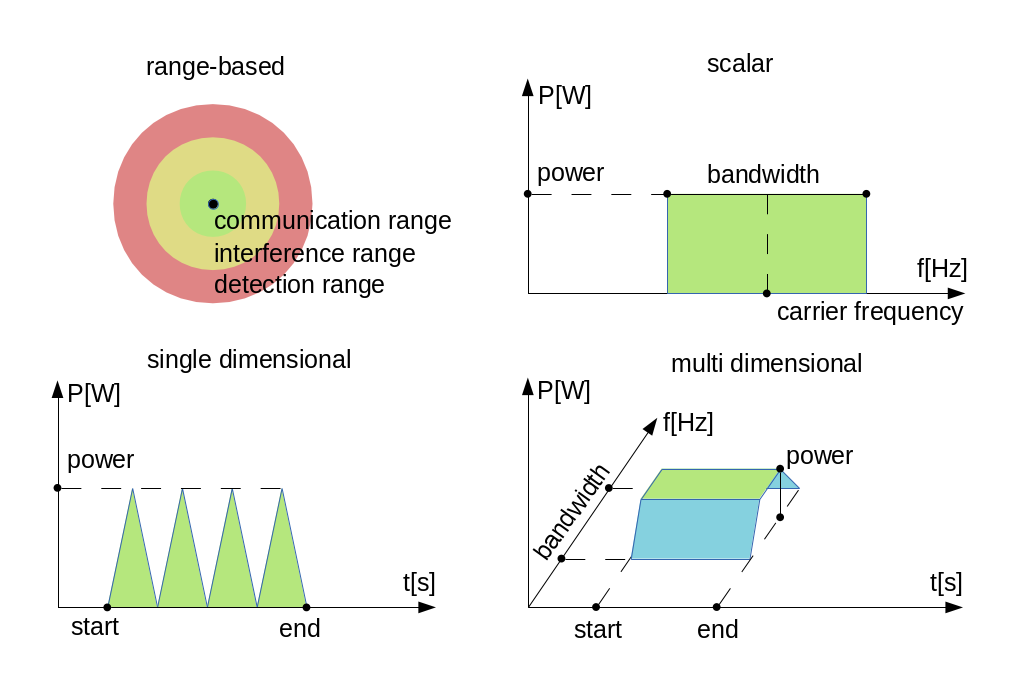
\includegraphics[width=\textwidth]{figures/phyanalog}
\caption{Various analog signal representations}
\end{figure}

The first representation is called range-based, and it's used by the unit disc
radio. The advantage of this data structure is that it's compact, predictable,
and provides high performance. The disadvantage is that it's very inaccurate in
terms of modeling reality. Nevertheless, this representation might be sufficient
for developing a new routing protocol if accurate simulation of packet loss is
not important.

The second data structure represents a narrowband signal with a scalar signal
power, a carrier frequency, and a bandwidth. The advantage of this
representation is that it allows to compute a real signal to noise ratio, which
in turn can be used by the error model to compute bit and packet error rates.
This representation is most of the time sufficient for the simulation of IEEE
802.11 networks.

The third data structure describes a signal power that changes over time. In
this case the signal power is represented with a one-dimensional time dependent
value that precisely follows the transmitted pulses. This representation is used
by the IEEE 802.15.4a UWB radio.

The last representation uses a multi-dimensional value to describe the signal
power that changes over both time and frequency. The IEEE 802.11b model might
use this representation to simulate crosstalk, where one channel interferes with
another. In order to make it work the frequency spectrum of the signal has to
follow the real spectrum more precisely at both ends of the band.

The flat signal representation uses a single object to simulatenously describe
all domains of the transmission or the reception. In contrast, the layered
signal representation uses one object to describe every domain seperately. The
advantage of the latter is that it's extensible with alternative implementations
for each domain. The disadvantage is that it needs more allocation and resource
management.

\section{Signal Processing}

The following figure shows the process of how a MAC packet gets from the
transmitter radio through the medium to the receiver radio. The figure focues on
how data flows between the processing components of the physical layer. The blue
boxes represent the data structures, and the red boxes represent the processing
components.

\begin{figure}[h!]
\centering
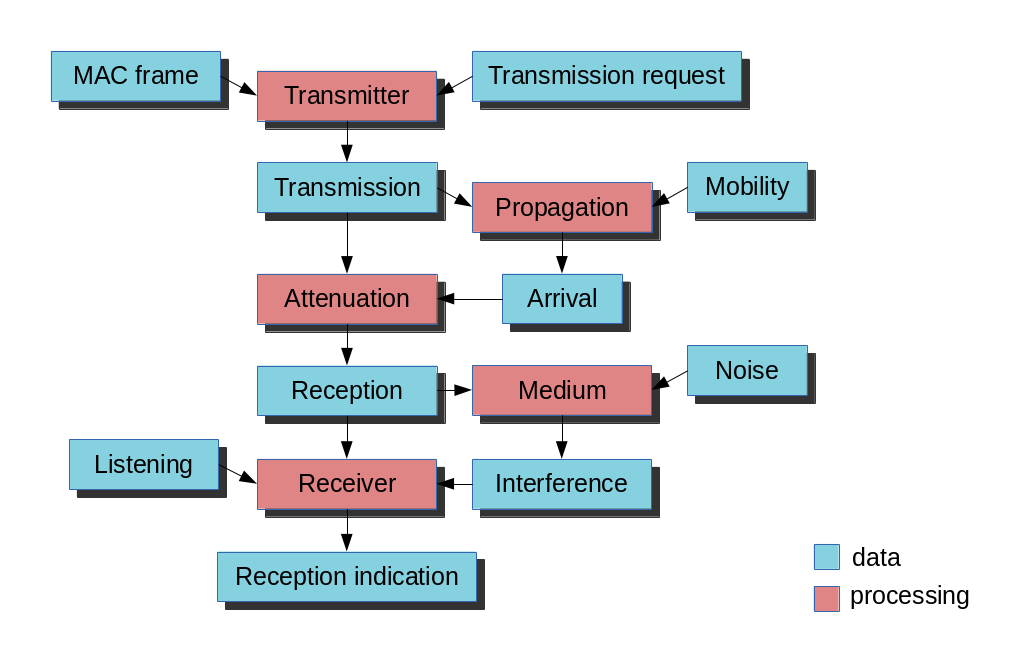
\includegraphics[width=\textwidth]{figures/phydataflow}
\caption{Signal processing data flow}
\end{figure}

The transmission process starts in the transmitter radio when it receives a MAC
packet from the higher layer. The radio must be in transmitter or transceiver
mode before receiving a MAC packet, otherwise it throws an exception. At first
the transmitter model creates a data structure that describes the transmitted
signal based on the received MAC packet and the attached transmission request.
The resulting data structure is immutable, it's not going to be changed in any
later processing step.

Thereafter the propagation model computes the arrival space-time coordinates for
all receivers. In the next step the medium model determines the set of affected
receivers. Which radio constitutes affected depends on a number of factors such
as the maximum communication range of the transmitter, the radio mode of the
receiver, the listening mode of the receiver, or potentially the MAC address of
the receiver. Using the result the medium model sends a separate message with
the shared transmission data structure to all affected receivers. There's no
need to send a message to all radios on the channel, because the computation
of interfering signals is independent of this step.

Thereafter the attenuation model computes the reception for the receiver using
the original transmission and the arrival data structure. It applies the path
loss model, the obstacle loss model and the multipath model to the transmission.
The resulting data structure is also immutable, it's not going to be changed in
any later processing step.

Thereafter the medium model computes the interference for the reception by
collecting all interfering receptions and noises. Another signal is considered
interfering if it owerlaps both in time and frequency domains with respect to 
the minimum interference parameters. The background noise model also computes a 
noise signal that is added to the interference.

The reception process starts in the receiver radio when it receives a message
from the transmitter radio. The radio must be in receiver or transceiver mode
before the message arrives, otherwise it ignores the message. At first the
receiver model determines is whether the reception is actually attempted or not.
This decision depends on the reception power, whether there's another ongoing
reception process, and capturing is enabled or not.

Thereafter the receiver model computes the signal to noise and interference
ratio from the reception and the interference. Using the result, the bitrate,
and the modulation scheme the error model computes the necessary error rates.
Alternatively the error model might compute the erroneous bits, or symbols by
altering the corresponding data of the original transmission. 

Thereafter the receiver determines the received MAC packet by either simply
reusing the original, or actually decoding from the lowest represented domain
in the reception. Finally, it attaches the physical layer indication to the MAC
packet, and sends it up to the higher layer.

The following sections describe the data structures that are created during
signal processing.

\subsubsection{Transmission Request}

This data structure contains parameters that control how the transmitter
produces the transmission. For example, it might override the default
transmission power, ot the default bitrate of the transmitter. It is attached as
a control info object to the MAC packet sent down from the MAC module to the
radio.

\subsubsection{Transmission}

This data structure describes the transmission of a signal. It specifies the
start/end time, start/end antenna position, start/end antenna orientation of the
transmitter. In other words, it describes when, where and how the signal
started/ended to interact with the medium. The transmitter model creates one
transmission instance per MAC packet.

\subsubsection{Arrival}

This data structure decscirbes the space and time coordinates of a transmission
arriving at a particular receiver. It specifies the start/end time, start/end
antenna position, start/end antenna orientation of the receiver. The propagation
model creates one arrival instance per transmission per receiver.

\subsubsection{Listening}

This data structure describes the way the receiver radio is listening on the
medium. The physical layer ignores certain transmissions either during computing
the interference or even the complete reception of such transmissions. For
example, a narrowband listening specifies a carrier frequency and a bandwidth. 

\subsubsection{Reception}

This data structure describes the reception of a signal by a particular receiver.
It specifies at least the start/end time, start/end antenna position, start/end
antenna orientation of the receiver. The attenuation model creates one reception
instance per transmission per receiver.

\subsubsection{Noise}

This data structure describes a meaningless signal or a meaningless composition
of multiple signals. All models contain at least the start/end time, and
start/end position.

\subsubsection{Interference}

This data structure describes the interfering signals and noises that affect a
particular reception. It also specifies the total noise that is the composition
of all interference.

\subsubsection{SNIR}

This data structure describes the signal to noise and interference ratio of a
particular reception. It also specifies the minimum signal to noise and
interference ratio.

\subsubsection{Reception Decision}

This data structure describes whether if the reception of a signal is possible
or not, is attempted or not, and is successful or not.

\subsubsection{Reception Indication}

This data structure describes the physical layer indications such as RSSI, SNIR,
PER, BER, SER. These physical properties are optional and may be omitted if the
receiver is configured to do so or if it doesn't support providing the data. The
reception indication is attached as a control info object to the MAC packet sent
up from the radio to the MAC module. 

\section{Visualization}

In order to help understanding the communication in the network the physical
layer supports visualizing its state. The following list shows what can be
displayed:

\begin{itemize}
  \item ongoing transmissions
  \item recent successful receptions
  \item recent obstacle intersections and surface normal vectors
\end{itemize}

The ongoing transmissions can be displayed with 3 dimensional spheres or with 2
dimensional rings laying in the XY plane. As the signal propagates through space
the figure grows with it to show where the beginning of the signal is. The inner
circle of the ring figure shows as the end of the signal propagates through
space. 

The recent successful receptions are displayed as straight lines between the
original positions of the transmission and the reception. The recent obstacle
intersections are also displayed as straight lines from the start of the
intersection to the end of it.

\ifdraft
\section{TODO other stuff}

TODO: scalar vs dimensional

TODO: flat vs layered

TODO: Generic, IEEE 802.11, IEEE 802.15.4

TODO: acoustic underwater example

TODO: wireless vs. wired medium

\section{Use Cases}

\fi



\cleardoublepage

\ifdraft TODO

\chapter{The 802.11 Model}
\label{cha:80211}


\section{Sending and Receiving 802.11 Frames}

TODO tags, etc.

\section{Architecture of the 802.11 MAC Model}

TODO

\fi



\cleardoublepage

\chapter{Node Mobility}
\label{cha:mobility}

\section{Overview}
\label{sec:mobility:overview}

In order to simulate ad-hoc wireless networks, it is important to model the
motion of mobile network nodes. Received signal strength, signal
interference, and channel occupancy depend on the distances between nodes.
The selected mobility models can significantly influence the results of the
simulation (e.g. via packet loss rates).

A mobility model describes position and orientation over time in a 3D
Euclidean coordinate system. Its main purpose is to provide position,
velocity and acceleration, and also angular position, angular velocity,
and angular acceleration data as three-dimensional quantities at the
current simulation time.

In INET, a mobility model is most often an OMNeT++ simple module
implementing the motion as a C++ algorithm. Although most models have a few
common parameters (e.g. for initial positioning), they always come with
their own set of parameters. Some models support geographic positioning to
ease the configuration of map based scenarios.

Mobility models be \textit{single} or \textit{group} mobility models.
Single mobility models describe the motion of entities independent of each other.
Group mobility models provide such a motion where group members are dependent
on each other.

Mobility models can also be categorized as \textit{trace-based},
\textit{deterministic}, \textit{stochastic}, and \textit{combining} models.

\subsection*{Using Mobility Models}

In order for a mobility model to actually have an effect on the motion of a network node,
the mobility model needs to be included as a submodule in the compound module of the
network node. By default, a transceiver antenna within a network node uses
the same mobility model as the node itself, but that is completely optional.
For example, it is possible to model a vehicle facing forward while moving
on a road that contains multiple transceiver antennas at different relative
locations with different orientations.

\subsection*{The Playground}

Many mobility models allow the user to define a cubic volume that the node
can not leave. The volume is configured by setting the \fpar{constraintAreaX},
\fpar{constraintAreaY}, \fpar{constraintAreaZ},
\fpar{constraintAreaWidth}, \fpar{constraintAreaHeight} and
\fpar{constraintAreaDepth} parameters.

If the \fpar{initFromDisplayString} parameter, the initial position is taken from
the display string. Otherwise, the position can be given in the \fpar{initialX},
\fpar{initialY} and \fpar{initialZ} parameters. If neither of these parameters
are given, a random initial position is choosen within the contraint area.

When the node reaches the boundary of the constraint area, the mobility
component has to prevent the node to exit. Many mobility models offer the
following policies:

\begin{itemize}
  \item reflect of the wall
  \item reappear at the opposite edge (torus area)
  \item placed at a randomly chosen position of the area
  \item stop the simulation with an error
\end{itemize}


\section{Built-In Mobility Models}
\label{sec:mobility:built-in-mobility-models}

\subsection{List of Mobility Models}
\label{sec:mobility:list-of-mobility-models}

The following, potentially list contains the mobility models available in INET.
Nearly all of these models als single mobility models; group mobility can be
implemented e.g. with combining other mobility models.

\subsubsection*{Stationary}

Stationary models only define position (and orientation), but no motion.

\begin{itemize}
    \item \nedtype{StationaryMobility} provides deterministic and random positioning.
    \item \nedtype{StaticGridMobility} places several mobility models in a rectangular grid.
    \item \nedtype{StaticConcentricMobility} places several models in a set of concentric circles.
\end{itemize}

\subsubsection*{Deterministic}

Deterministic mobility models use non-random mathematical models for describing motion.

\begin{itemize}
    \item \nedtype{LinearMobility} moves linearly with a constant speed or constant acceleration.
    \item \nedtype{CircleMobility} moves around a circle parallel to the XY plane with constant speed.
    \item \nedtype{RectangleMobility} moves around a rectangular area parallel to the XY plane with constant speed.
    \item \nedtype{TractorMobility} moves similarly to a tractor on a field with a number of rows.
    \item \nedtype{VehicleMobility} moves similarly to a vehicle along a path especially turning around corners.
    \item \nedtype{TurtleMobility} moves according to an XML script written in a simple yet expressive LOGO-like programming language.
    \item \nedtype{FacingMobility} orients towards the position of another mobility model.
    \item \nedtype{RotatingMobility} rotates with a constant speed.
\end{itemize}

\subsubsection*{Trace-Based}

Trace-based mobility models replay recorded motion as observed in real life.

\begin{itemize}
    \item \nedtype{BonnMotionMobility} replays trace files of the BonnMotion scenario generator.
    \item \nedtype{Ns2MotionMobility} replays files of the CMU's scenario generator used in ns2.
    \item \nedtype{AnsimMobility} replays XML trace files of the ANSim (Ad-Hoc Network Simulation) tool.
\end{itemize}

\subsubsection*{Stochastic}

Stochastic or random mobility models use mathematical models involving random numbers.

\begin{itemize}
    \item \nedtype{RandomWaypointMobility} moves to random destination with random speed.
    \item \nedtype{GaussMarkovMobility} uses one parameter to vary the degree of randomness from linear to Brown motion.
    \item \nedtype{MassMobility} moves similarly to a mass with inertia and momentum.
    \item \nedtype{ChiangMobility} uses a probabilistic transition matrix to change the motion state.
\end{itemize}

\subsubsection*{Combining}

Combining mobility models are not mobility models per se, but instead, they
allow more complex motions to be formed from simpler ones via superposition
and other ways.

\begin{itemize}
        \item \nedtype{SuperpositioningMobility} model combines several other mobility models by summing them up. It allows creating group mobility by sharing a mobility model in each group member, separating initial positioning from positioning during the simulation, and separating positioning from orientation.
        \item \nedtype{AttachedMobility} models a mobility that is attached to another one at a given offset. Position, velocity and acceleration are all affected by the respective quantites and also the orientation of the referenced mobility.
\end{itemize}

\subsection{More Information on Some Mobility Models}
\label{sec:mobility:more-information-on-some-mobility-models}

\subsubsection*{TractorMobility}

Moves a tractor through a field with a certain
amount of rows. The following figure illustrates the movement of the
tractor when the \fpar{rowCount} parameter is 2. The trajectory follows
the segments in $1,2,3,4,5,6,7,8,1,2,3\ldots$ order. The area is configured
by the \fpar{x1}, \fpar{y1}, \fpar{x2}, \fpar{y2} parameters.

% TODO use constraint area instead of new x1,y1,x2,y2 parameters as in RectangleMobility

\begin{pdfonly}
\begin{center}
\setlength{\unitlength}{0.5mm}
\begin{picture}(80,80)
\put(40,72){$1$} \put(10,70){\vector(1,0){30}} \put(10,70){\line(1,0){60}}
\put(72,55){$2$} \put(70,70){\vector(0,-1){15}} \put(70,70){\line(0,-1){30}}
\put(40,42){$3$} \put(70,40){\vector(-1,0){30}} \put(70,40){\line(-1,0){60}}
\put(5,25){$4$} \put(10,40){\vector(0,-1){15}} \put(10,40){\line(0,-1){30}}
\put(40,12){$5$} \put(10,10){\vector(1,0){30}} \put(10,10){\line(1,0){60}}
\put(72,25){$6$} \put(70,10){\vector(0,1){15}} \put(70,10){\line(0,1){30}}
\put(40, 33){$7$}
\put(5,55){$8$} \put(10,40){\vector(0,1){15}} \put(10,40){\line(0,1){30}}
\put(0,72){$(x_1,y_1)$} \put(65,2){$(x_2,y_2)$}
\end{picture}
\end{center}
\end{pdfonly}

\begin{htmlonly}
<center><img src="tractormobility.png" border="0" width="240"></center> <!-- screenshot from the PDF version -->
\end{htmlonly}

\subsubsection*{RandomWaypointMobility}

In the Random Waypoint mobility model the nodes move in line segments. For each
line segment, a random destination position (distributed uniformly over the
playground) and a random speed is chosen. You can define a speed as a variate
from which a new value will be drawn for each line segment; it is customary to
specify it as \ttt{uniform(minSpeed, maxSpeed)}. When the node reaches the
target position, it waits for the time \fpar{waitTime} which can also be defined as a
variate. After this time the the algorithm calculates a new random position, etc.

\subsubsection*{GaussMarkovMobility}

The Gauss-Markov model contains a tuning parameter that control the randomness
in the movement of the node. Let the magnitude and direction of speed of the
node at the $n$th time step be $s_n$ and $d_n$. The next speed and direction are
computed as

$$ s_{n+1} = \alpha s_n + (1 - \alpha) \bar{s} + \sqrt{(1-\alpha^2)} s_{x_n} $$

$$ d_{n+1} = \alpha s_n + (1 - \alpha) \bar{d} + \sqrt{(1-\alpha^2)} d_{x_n} $$

where $\bar{s}$ and $\bar{d}$ are constants representing the mean value
of speed and direction as $n \to \infty$; and $s_{x_n}$ and $d_{x_n}$
are random variables with Gaussian distribution.

Totally random walk (Brownian motion) is obtained by setting $\alpha=0$,
while $\alpha=1$ results a linear motion.

To ensure that the node does not remain at the boundary of the constraint
area for a long time, the mean value of the direction ($\bar{d}$) modified
as the node enters the margin area. For example at the right edge of the
area it is set to 180 degrees, so the new direction is away from the edge.

% FIXME the GaussMarkovMobility module has only one variance parameter.
%       it should have separate speed and direction parameters

\subsubsection*{MassMobility}

This is a random mobility model for a mobile host with
a mass. It is the one used in \cite{Perkins99optimizedsmooth}.

\begin{quote}
"An MH moves within the room according to the following pattern. It moves
along a straight line for a certain period of time before it makes a turn.
This moving period is a random number, normally distributed with average of
5 seconds and standard deviation of 0.1 second. When it makes a turn, the
new direction (angle) in which it will move is a normally distributed
random number with average equal to the previous direction and standard
deviation of 30 degrees. Its speed is also a normally distributed random
number, with a controlled average, ranging from 0.1 to 0.45 (unit/sec), and
standard deviation of 0.01 (unit/sec). A new such random number is picked
as its speed when it makes a turn. This pattern of mobility is intended to
model node movement during which the nodes have momentum, and thus do not
start, stop, or turn abruptly. When it hits a wall, it reflects off the
wall at the same angle; in our simulated world, there is little other
choice."
\end{quote}

This implementation can be parameterized a bit more, via the
\fpar{changeInterval}, \fpar{changeAngleBy} and \fpar{changeSpeedBy} parameters.
The parameters described above correspond to the following settings:

\begin{itemize}
\item changeInterval = normal(5, 0.1)
\item changeAngleBy = normal(0, 30)
\item speed = normal(avgSpeed, 0.01)
\end{itemize}

\subsubsection*{ChiangMobility}

Implements Chiang's random walk movement model (\cite{Chiang98wirelessnetwork}).
In this model, the state of the mobile node in each direction (x and y) can be:

\begin{itemize}
  \item 0: the node stays in its current position
  \item 1: the node moves forward
  \item 2: the node moves backward
\end{itemize}

The $(i,j)$ element of the state transition matrix determines the
probability that the state changes from $i$ to $j$:

\begin{pdfonly}
$$ \left(
\begin{array}{ccc}
  0 & 0.5 & 0.5 \\
  0.3 & 0.7 & 0 \\
  0.3 & 0 & 0.7
\end{array}
\right) $$
\end{pdfonly}

\begin{htmlonly}
<center>
<div>
<table class="matrix">
  <tr> <td>0</td>   <td>0.5</td> <td>0.5</td> </tr>
  <tr> <td>0.3</td> <td>0.7</td> <td>0</td>   </tr>
  <tr> <td>0.3</td> <td>0</td>   <td>0.7</td> </tr>
</table>
</div>
</center>
\end{htmlonly}

\subsection{Replaying trace files}
\label{sec:mobility:replaying-trace-files}

\subsubsection*{BonnMotionMobility}

Uses the native file format of \href{http://bonnmotion.net}{BonnMotion}.

The file is a plain text file, where every line describes the motion
of one host. A line consists of one or more (t, x, y) triplets of real
numbers, like:

\begin{verbatim}
t1 x1 y1 t2 x2 y2 t3 x3 y3 t4 x4 y4 ...
\end{verbatim}

The meaning is that the given node gets to $(xk,yk)$ at $tk$. There's no
separate notation for wait, so x and y coordinates will be repeated there.

\subsubsection*{Ns2MotionMobility}

Nodes are moving according to the trace files used in NS2.
The trace file has this format:

\begin{verbatim}
# '#' starts a comment, ends at the end of line
$node_(<id>) set X_ <x> # sets x coordinate of the node identified by <id>
$node_(<id>) set Y_ <y> # sets y coordinate of the node identified by <id>
$node_(<id>) set Z_ <z> # sets z coordinate (ignored)
$ns at $time "$node_(<id>) setdest <x> <y> <speed>" # at $time start moving
towards <x>,<y> with <speed>
\end{verbatim}

The \nedtype{Ns2MotionMobility} module has the following parameters:

\begin{itemize}
  \item \fpar{traceFile} the Ns2 trace file
  \item \fpar{nodeId} node identifier in the trace file; -1 gets substituted by
  parent module's index
  \item \fpar{scrollX},\fpar{scrollY} user specified translation of the
  coordinates
\end{itemize}

% TODO cleaning the code (e.g. duplicated bounds check in setTargetPosition())
% TODO implement cached file access as in BonnMotionMobility

\subsubsection*{ANSimMobility}

It reads trace files of the \href{http://www.ansim.info}{ANSim} Tool.
The nodes are moving along linear segments described by an XML trace file
conforming to this DTD:

\begin{XML}
<!ELEMENT mobility (position_change*)>
<!ELEMENT position_change (node_id, start_time, end_time, destination)>
<!ELEMENT node_id (#PCDATA)>
<!ELEMENT start_time (#PCDATA)>
<!ELEMENT end_time (#PCDATA)>
<!ELEMENT destination (xpos, ypos)>
<!ELEMENT xpos (#PCDATA)>
<!ELEMENT ypos (#PCDATA)>
\end{XML}

Parameters of the module:

\begin{itemize}
  \item \fpar{ansimTrace} the trace file
  \item \fpar{nodeId} the \verb!node_id! of this node, -1 gets substituted to
  parent module's index
\end{itemize}

\begin{note}
The \nedtype{AnsimMobility} module processes only the \ttt{position\_change}
elements and it ignores the \ttt{start\_time} attribute. It starts the move
on the next segment immediately.
\end{note}

\subsection{TurtleMobility}
\label{sec:mobility:turtlemobility}

The \nedtype{TurtleMobility} module can be parametrized by a script file
containing LOGO-style movement commands in XML format. The content of
the XML file should conform to the DTD in the \ffilename{TurtleMobility.dtd}
file in the source tree.

The file contains \ttt{movement} elements, each describing a trajectory.
The \ttt{id} attribute of the \ttt{movement} element can be used to
refer the movement from the ini file using the syntax:

\begin{inifile}
**.mobility.turtleScript = xmldoc("turtle.xml", "movements//movement[@id='1']")
\end{inifile}

The motion of the node is composed of uniform linear segments.
The \ttt{movement} elements may contain the the following commands as
elements (names in parens are recognized attribute names):

\begin{itemize}
\item \ttt{repeat(n)} repeats its content n times, or indefinitely if
       the \ttt{n} attribute is omitted.
\item \ttt{set(x,y,speed,angle,borderPolicy)} modifies the state of the node.
      \ttt{borderPolicy} can be \ttt{reflect}, \ttt{wrap}, \ttt{placerandomly}
      or \ttt{error}.
\item \ttt{forward(d,t)} moves the node for $t$ time or to the $d$ distance
      with the current speed. If both $d$ and $t$ is given, then the current
      speed is ignored.
\item \ttt{turn(angle)} increase the angle of the node by $angle$ degrees.
\item \ttt{moveto(x,y,t)} moves to point $(x,y)$ in the given time. If
      $t$ is not specified, it is computed from the current speed.
\item \ttt{moveby(x,y,t)} moves by offset $(x,y)$ in the given time. If
      $t$ is not specified, it is computed from the current speed.
\item \ttt{wait(t)} waits for the specified amount of time.
\end{itemize}

Attribute values must be given without physical units, distances are assumed
to be given as meters, time intervals in seconds and speeds in meter per seconds.
Attibutes can contain expressions that are evaluated each time the
command is executed. The limits of the constraint area can be
referenced as \verb!$MINX!, \verb!$MAXX!, \verb!$MINY!, and \verb!$MAXY!.
Random number distibutions generate a new random number when evaluated,
so the script can describe random as well as deterministic scenarios.

To illustrate the usage of the module, we show how some mobility
models can be implemented as scripts.

RectangleMobility:

\begin{XML}
<movement>
    <set x="$MINX" y="$MINY" angle="0" speed="10"/>
    <repeat>
        <repeat n="2">
            <forward d="$MAXX-$MINX"/>
            <turn angle="90"/>
            <forward d="$MAXY-$MINY"/>
            <turn angle="90"/>
        </repeat>
    </repeat>
</movement>
\end{XML}

Random Waypoint:

\begin{XML}
<movement>
    <repeat>
        <set speed="uniform(20,60)"/>
        <moveto x="uniform($MINX,$MAXX)" y="uniform($MINY,$MAXY)"/>
        <wait t="uniform(5,10)">
    </repeat>
</movement>
\end{XML}

MassMobility:

\begin{XML}
<movement>
    <repeat>
        <set speed="uniform(10,20)"/>
        <turn angle="uniform(-30,30)"/>
        <forward t="uniform(0.1,1)"/>
    </repeat>
</movement>
\end{XML}


%%% Local Variables:
%%% mode: latex
%%% TeX-master: "usman"
%%% End:



\cleardoublepage

\chapter{The IPv4 Protocol Family}
\label{cha:ipv4}


\section{Overview}
\label{sec:ipv4:overview}

The IP protocol is the workhorse protocol of the TCP/IP protocol suite.
All UDP, TCP, ICMP packets are encapsulated into IP datagrams and
transported by the IP layer.
While higher layer protocols transfer data among two communication end-point,
the IP layer provides an hop-by-hop, unreliable and connectionless delivery
service. IP does not maintain any state information about the individual
datagrams, each datagram handled independently.

The nodes that are connected to the Internet can be either a host or a router.
The hosts can send and recieve IP datagrams, and their operating system
implements the full TCP/IP stack including the transport layer. On the
other hand, routers have more than one interface cards and perform packet
routing between the connected networks. Routers does not need the
transport layer, they work on the IP level only. The division
between routers and hosts is not strict, because if a host
have several interfaces, they can usually be configured to operate
as a router too.

Each node on the Internet has a unique IP address. IP datagrams contain
the IP address of the destination. The task of the routers is to find
out the IP address of the next hop on the local network, and forward
the packet to it. Sometimes the datagram is larger, than the maximum
datagram that can be sent on the link (e.g. Ethernet has an 1500 bytes limit.).
In this case the datagram is split into fragments and each fragment is
transmitted independently. The destination host must collect all fragments,
and assemble the datagram, before sending up the data to the transport
layer.

The INET framework contains several modules to build the IPv4 network layer of
hosts and routers:

\begin{itemize}
  \item \nedtype{Ipv4} is the main module that implements RFC791. This
        module performs IP encapsulation/decapsulation, fragmentation
        and assembly, and routing of IP datagrams.
  \item The \nedtype{Ipv4RoutingTable} is a helper module that manages the routing
        table of the node. It is queried by the \nedtype{Ipv4} module
        for best routes, and updated by the routing daemons implementing
        RIP, OSPF, Manet, etc. protocols.
  \item The \nedtype{Icmp} module can be used to generate ICMP error packets. It also
        supports ICMP echo applications.
  \item The \nedtype{Arp} module performs the dynamic translation of IP addresses
        to MAC addresses.
  \item The \nedtype{Igmpv2} module to generate and process multicast group
        membership reports.
\end{itemize}

These modules are assembled into a complete network layer module called
\nedtype{Ipv4NetworkLayer}. The \nedtype{Ipv4NetworkLayer} module is present
e.g. in \nedtype{StandardHost} and \nedtype{Router}.

The subsequent sections describe the IPv4 modules in detail.

\section{Ipv4}
\label{sec:ipv4:ipv4}

The \nedtype{Ipv4} module implements the IPv4 protocol.

Its parameters include:

\begin{itemize}
  \item \fpar{crcMode} TODO: @enum("declared", "computed") = default("declared");
  \item \fpar{procDelay} processing time of each incoming datagram.
  \item \fpar{timeToLive} default TTL of unicast datagrams.
  \item \fpar{multicastTimeToLive} default TTL of multicast datagrams.
  \item \fpar{fragmentTimeout} the maximum duration until fragments are kept
          in the fragment buffer.
  \item \fpar{forceBroadcast} if \fkeyword{true}, then link-local broadcast
          datagrams are sent out through each interface, if the higher
          layer did not specify the outgoing interface.
  \item \fpar{useProxyARP} TODO: default(true);
\end{itemize}

\section{Ipv4RoutingTable}
\label{sec:ipv4:ipv4routingtable}

The \nedtype{Ipv4RoutingTable} module represents the IPv4 route table.
Hosts and routers normally contain one instance of this module.
The \nedtype{Ipv4RoutingTable} module does not send or receive messages.
Instead, C++ methods are for querying and updating the table, as well as for
unicast and multicast routing.

The \nedtype{Ipv4RoutingTable} module has the following parameters:

\begin{itemize}
  \item \fpar{routerId}: for routers, the router id using IPv4 address dotted notation;
      specify ``auto'' to select the highest interface address; should be left empty ``''
      for hosts.
  \item \fpar{forwarding}: turns IP forwarding on/off. It is always \ttt{true}
      in a \nedtype{Router} and is \ttt{false} by default in a \nedtype{StandardHost}.
  \item \fpar{multicastForwarding}: turns multicast IP forwarding on/off.
    Default is \fkeyword{false}, should be set to \fkeyword{true} in multicast routers.
\end{itemize}

The preferred method for static initialization of routing tables is to use
\nedtype{Ipv4NetworkConfigurator}. While \nedtype{Ipv4RoutingTable}
can read the routes from a \textit{routing file}, that is considered obsolete.
Old routing files should be replaced with the XML configuration of
\nedtype{Ipv4NetworkConfigurator}. Section \ref{subsec:ipv4configurator}
describes the format of the new configuration files.


\section{Icmp}
\label{sec:ipv4:icmp}

The \nedtype{Icmp} module implements the Internet Control Message Protocol
(ICMP). ICMP is the error reporting and diagnostic mechanism of the Internet.
It uses the services of IP, so it is a transport layer protocol, but unlike TCP
or UDP it is not used to transfer user data. It cannot be separated from
IP, because the routing errors are reported by ICMP.

The \nedtype{Icmp} module can be used to send error messages and ping
request. It can also respond to incoming ICMP messages.

Each ICMP message is encapsulated within an IP datagram, so its delivery
is unreliable.

\section{Arp}
\label{sec:ipv4:arp}

The \nedtype{Arp} module implements the Address Resolution Protocol (ARP).
The ARP protocol is designed to translate a local protocol address to a hardware
address. Although the ARP protocol can be used with several network protocol and
hardware addressing schemes, in practice they are almost always IPv4 and 802.3
addresses. The \nedtype{Arp} module only supports IPv4-to-MAC address
translation, but not the opposite direction, Reverse ARP (RARP).

The address to be resolved can be either an IPv4 broadcast/multicast or a
unicast address. The corresponding MAC addresses can be computed for broadcast
and multicast addresses (RFC 1122, 6.4); unicast addresses are resolved
using the ARP procotol.

If the MAC address is found in the ARP cache, then the packet is transmitted to
the addressed interface immediately. Otherwise the packet is queued and an
address resolution takes place.

For address resolution, ARP broadcasts a request frame on the network. In the
request it publishes its own IP and MAC addresses, so each node in the local
subnet can update their mapping. The node whose MAC address was requested will
respond with an ARP frame containing its own MAC address directly to the node
that sent the request. When the original node receives the ARP response, it
updates its ARP cache and sends the delayed IP packet using the learned MAC
address.

ARP resolution is initiated with a C++ call.

The module parameters of \nedtype{Arp} are:

\begin{itemize}
  \item \fpar{retryTimeout}: number of seconds ARP waits between retries to resolve an IPv4 address (default is 1s)
  \item \fpar{retryCount}: number of times ARP will attempt to resolve an IPv4 address (default is 3)
  \item \fpar{cacheTimeout}: number of seconds unused entries in the cache will time out (default is 120s)
  \item \fpar{proxyARP}: enables proxy ARP mode (default is \fkeyword{true})
  \item \fpar{globalARP}: use global ARP cache (default is \fkeyword{false})
\end{itemize}


\section{Igmp}
\label{sec:ipv4:igmp}

The \nedtype{Igmp} module implements the Internet Group Management Protocol
(IGMP). IGMP is a communications protocol used by hosts and adjacent routers on
IPv4 networks to establish multicast group memberships. IGMP is an integral part
of IP multicast.

IGMP is responsible for distributing the information of
multicast group memberships from hosts to routers. When an interface
of a host joins to a multicast group, it will send an IGMP report
on that interface to routers. It can also send reports when the
interface leaves the multicast group, so it does not want to
receive those multicast datagrams. The IGMP module of multicast
routers processes these IGMP reports: it updates the list of
groups, that has members on the link of the incoming message.

The \nedtype{IIgmp} module interface defines the connections
of IGMP modules.
IGMP reports are transmitted by IP, so the module contains
gates to be connected to the IP module (\ttt{ipIn/ipOut}). The IP
module delivers packets with protocol number 2 to the IGMP module.
However some multicast routing protocols (like DVMRP) also exchange
routing information by sending IGMP messages, so they should be
connected to the \ttt{routerIn/routerOut} gates of the IGMP module.
The IGMP module delivers the IGMP messages not processed by itself
to the connected routing module.

The \nedtype{Igmpv2} module implements version 2 of the IGMP protocol
(RFC 2236). Next we describe its behaviour in host and routers in details.
Note that multicast routers behaves as hosts too, i.e. they are sending
reports to other routers when joining or leaving a multicast group.

\subsection*{Host behaviour}

When an interface joins to a multicast group, the host
will send a Membership Report immediately to the group address.
This report is repeated after \fpar{unsolicitedReportInterval} to
cover the possibility of the first report being lost.

When a host's interface leaves a multicast group, and it was
the last host that sent a Membership Report for that group,
it will send a Leave Group message to the all-routers multicast
group (224.0.0.2).

This module also responds to IGMP Queries. When the host
receives a Group-Specific Query on an interface that belongs
to that group, then it will set a timer to a random value
between 0 and Max Response Time of the Query. If the timer
expires before the host observe a Membership Report sent
by other hosts, then the host sends an IGMPv2 Membership Report.
When the host receives a General Query on an interface,
a timer is initialized and a report is sent for each group
membership of the interface.

\subsection*{Router behaviour}

Multicast routers maintains a list for each interface containing
the multicast groups that have listeners on that interface.
This list is updated when IGMP Membership Reports and Leave Group
messages arrive, or when a timer expires since the last Query.

When multiple routers are connected to the same link, the one with
the smallest IP address will be the Querier. When other routers
observe that they are Non-Queriers (by receiving an IGMP Query
with a lower source address), they stop sending IGMP Queries
until \fpar{otherQuerierPresentInterval} elapsed since the last
received query.

Routers periodically (\fpar{queryInterval}) send a General Query
on each attached network for which this router is a Querier.
On startup the router sends \fpar{startupQueryCount} queries
separated by \fpar{startupQueryInterval}. A General Query
has unspecified Group Address field, a Max Response Time
field set to \fpar{queryResponseInterval}, and is sent to the
all-systems multicast address (224.0.0.1).

When a router receives a Membership Report, it will add the
reported group to the list of multicast group memberships.
At the same time it will set a timer for the membership
to \fpar{groupMembershipInterval}. Repeated reports restart
the timer. If the timer expires, the router assumes
that the group has no local members, and multicast traffic
is no more forwarded to that interface.

When a Querier receives a Leave Group message for a group,
it sends a Group-Specific Query to the group being left.
It repeats the Query \fpar{lastMemberQueryCount} times in
separated by \fpar{lastMemberQueryInterval} until a Membership
Report is received. If no Report received, then the router
assumes that the group has no local members.

% FIXME IGMPv2 not compatible with IGMPv1 hosts and routers

\subsection*{Parameters}

The following parameters have effects in both hosts and routers:

\begin{itemize}
  \item \fpar{enabled} if \fkeyword{false} then the IGMP module
     never sends any message and discards incoming messages.
  Default is \fkeyword{true}.
\end{itemize}

The following parameters are only used in hosts:

\begin{itemize}
  \item \fpar{unsolicitedReportInterval} the time between repetitions of a
   host's initial report of membership in a group. Default is 10s.
\end{itemize}

Router timeouts are configured by these parameters:

\begin{itemize}
  \item \fpar{robustnessVariable} the IGMP is robust to \fpar{robustnessVariable}-1
   packet losses. Default is 2.
  \item \fpar{queryInterval} the interval between General Queries sent by a Querier.
   Default is 125s.
  \item \fpar{queryResponseInterval} the Max Response Time inserted into General Queries
  \item \fpar{groupMembershipInterval} the amount of time that must pass before
   a multicast router decides there are no more members of a group on a network.
   Fixed to \fpar{robustnessVariable} * \fpar{queryInterval} + \fpar{queryResponseInterval}.
  \item \fpar{otherQuerierPresentInterval} the length of time that must
   pass before a multicast router decides that there is no longer
   another multicast router which should be the querier.
   Fixed to \fpar{robustnessVariable} * \fpar{queryInterval} + \fpar{queryResponseInterval} / 2.
  \item \fpar{startupQueryInterval} the interval between General Queries
   sent by a Querier on startup. Default is \fpar{queryInterval} / 4.
  \item \fpar{startupQueryCount} the number of Queries sent out on startup,
   separated by the \fpar{startupQueryInterval}. Default is \fpar{robustnessVariable}.
  \item \fpar{lastMemberQueryInterval} the Max Response Time inserted into
   Group-Specific Queries sent in response to Leave Group messages, and
   is also the amount of time between Group-Specific Query messages.
   Default is 1s.
  \item \fpar{lastMemberQueryCount} the number of Group-Specific Queries
   sent before the router assumes there are no local members.
   Default is \fpar{robustnessVariable}.
\end{itemize}


%%% Local Variables:
%%% mode: latex
%%% TeX-master: "usman"
%%% End:


\cleardoublepage

\chapter{IPv6 and Mobile IPv6}
\label{cha:ipv6}


\section{Overview}
\label{sec:ipv6:overview}

IPv6 support is implemented by several cooperating modules. The IPv6 module
implements IPv6 datagram handling (sending, forwarding etc). It relies on
\nedtype{Ipv6RoutingTable} to get access to the routes. \nedtype{Ipv6RoutingTable} also contains the
neighbour discovery data structures (destination cache, neighbour cache,
prefix list -- the latter effectively merged into the route table). Interface
configuration (address, state, timeouts etc) is held in the \nedtype{InterfaceTable},
in \cppclass{Ipv6InterfaceData} objects attached to \cppclass{InterfaceEntry}
as its \ttt{ipv6()} member.

The module \nedtype{Ipv6NeighbourDiscovery} implements all tasks associated with
neighbour discovery and stateless address autoconfiguration. The data
structures themselves (destination cache, neighbour cache, prefix list)
are kept in \nedtype{Ipv6RoutingTable}, and are accessed via public C++ methods.
Neighbour discovery packets are only sent and processed by this module --
when IPv6 receives one, it forwards the packet to \nedtype{Ipv6NeighbourDiscovery}.

The rest of ICMPv6 (ICMP errors, echo request/reply etc) is implemented in
the module \nedtype{Icmpv6}, just like with IPv4. ICMP errors are sent into
\nedtype{Ipv6ErrorHandling}, which the user can extend or replace to get errors
handled in any way they like.


%%% Local Variables:
%%% mode: latex
%%% TeX-master: "usman"
%%% End:


\cleardoublepage

\ifdraft TODO

\chapter{The Netfilter API}
\label{cha:netfilter-api}

\section{Overview}

TODO

\fi

\cleardoublepage

\ifdraft TODO

\chapter{The UDP Model}
\label{cha:udp}

\section{The UDP module}

The state of the sockets are stored within the UDP module and the application
can configure the socket by sending command messages to the UDP module.
These command messages are distinguished by their kind and the type of their
control info. The control info identifies the socket and holds the parameters
of the command.

Applications don't have to send messages directly to the UDP module,
as they can use the \cppclass{UdpSocket} utility class, which encapsulates the messaging and
provides a socket like interface to applications.

\subsection{Sending UDP datagrams}

If the application want to send datagrams, it optionally can connect to the destination.
It does this be sending a message with UDP\_C\_CONNECT kind and \cppclass{UdpConnectCommand}
control info containing the remote address and port of the connection.
The UDP protocol is in fact connectionless, so it does not send any packets as a result
of the connect call. When the UDP module receives the connect request,
it simply remembers the destination address and port and use it as default destination
for later sends. The application can send several connect commands to the same socket.

% FIXME currently connect() or bind() is mandatory as the first command,
%       the application cannot send packets or set options otherwise

% FIXME connect() should allow unspecified dest address and -1 port (interpreted as disconnect())

For sending an UDP packet, the application should attach an \cppclass{UDPSendCommand}
control info to the packet, and send it to \nedtype{Udp}. The control info may contain
the destination address and port. If the destination address or port
is unspecified in the control info then the packet is sent to the connected target.

The \nedtype{Udp} module encapsulates the application's packet into an \msgtype{UDPPacket},
creates an appropriate IP control info and send it over ipOut or ipv6Out depending on
the destination address.

The destination address can be the IPv4 local broadcast address (255.255.255.255)
or a multicast address. Before sending broadcast messages, the socket must be configured
for broadcasting. This is done by sending an message to the UDP module. The message
kind is UDP\_C\_SETOPTION and its control info (an \cppclass{UdpSetBroadcastCommand})
tells if the broadcast is enabled. You can limit the multicast to the local network
by setting the TTL of the IP packets to 1. The TTL can be configured per socket,
by sending a message to the UDP with an \cppclass{UDPSetTimeToLive} control info
containing the value. If the node has multiple interfaces, the application can
choose which is used for multicast messages. This is also a socket option, the
id of the interface (as registered in the interface table) can be given in an
\cppclass{UdpSetMulticastInterfaceCommand} control info.

% FIXME currently sending broadcast messages is enabled without setting SO_BROADCAST to true,
%       this is not so in UNIX

% FIXME there should be a separate TTL for multicast (not used for unicast), default value is 1
%       see IP_MULTICAST_TTL in `man 7 ip`

\begin{note}
The \nedtype{Udp} module supports only local broadcasts (using the special 255.255.255.255 address).
Packages that are broadcasted to a remote subnet are handled as undeliverable messages.
\end{note}

If the UDP packet cannot be delivered because nobody listens on the destination port,
the application will receive a notification about the failure. The notification is
a message with UDP\_I\_ERROR kind having attached an \cppclass{UdpErrorIndication}
control info. The control info contains the local and destination address/port,
but not the original packet.

After the application finished using a socket, it should close it by sending a message
UDP\_C\_CLOSE kind and \cppclass{UdpCloseCommand} control info. The control info
contains only the socket identifier. This command frees the resources associated
with the given socket, for example its socket identifier or bound address/port.

\subsection{Receiving UDP datagrams}

Before receiving UDP datagrams applications should first ``bind'' to the given UDP port.
This can be done by sending a message with message kind UDP\_C\_BIND attached with an
\cppclass{UdpBindCommand} control info. The control info contains the socket identifier
and the local address and port the application want to receive UDP packets.
Both the address and port is optional. If the address is unspecified, than the UDP
packets with any destination address is passed to the application. If the port is
-1, then an unused port is selected automatically by the UDP module.
The localAddress/localPort combination must be unique.

When a packet arrives from the network, first its error bit is checked. Erronous messages
are dropped by the UDP component. Otherwise the application bound to the destination port
is looked up, and the decapsulated packet passed to it. If no application is bound to
the destination port, an ICMP error is sent to the source of the packet. If the socket is
connected, then only those packets are delivered to the application, that received from
the connected remote address and port.

The control info of the decapsulated packet is an \cppclass{UDPDataIndication}
and contains information about the source and destination address/port, the TTL,
and the identifier of the interface card on which the packet was received.

The applications are bound to the unspecified local address, then they receive any packets
targeted to their port. UDP also supports multicast and broadcast addresses; if they
are used as destination address, all nodes in the multicast group or subnet receives the packet.
The socket receives the broadcast packets only if it is configured for broadcast.
To receive multicast messages, the socket must join to the group of the multicast address.
This is done be sending the UDP module an UDP\_C\_SETOPTION message with
\cppclass{UdpJoinMulticastGroupsCommand} control info. The control info specifies the
multicast addresses and the interface identifiers. If the interface identifier is given
only those multicast packets are received that arrived at that interface.
The socket can stop receiving multicast messages if it leaves the multicast group.
For this purpose the application should send the UDP another UDP\_C\_SETOPTION
message in their control info (\cppclass{UdpLeaveMulticastGroupsCommand}) specifying
the multicast addresses of the groups.

% TODO clarify: multicast packets should not be delivered to connected sockets?

\subsection{Signals}

The \nedtype{Udp} module emits the following signals:
\begin{itemize}
  \item \fsignal{sentPk} when an UDP packet sent to the IP, the packet
  \item \fsignal{rcvdPk} when an UDP packet received from the IP, the packet
  \item \fsignal{passedUpPk} when a packet passed up to the application, the packet
  \item \fsignal{droppedPkWrongPort} when an undeliverable UDP packet received, the packet
  \item \fsignal{droppedPkBadChecksum} when an erronous UDP packet received, the packet
\end{itemize}

\fi



\cleardoublepage

\ifdraft TODO

\chapter{The TCP Models}
\label{cha:tcp}

\section{The TCP Module}

The \nedtype{Tcp} model relies on sending and receiving \cppclass{IPControlInfo} objects
attached to TCP segment objects as control info (see \ffunc{cMessage::setControlInfo()}).

The \nedtype{Tcp} module manages several \cppclass{TcpConnection} object each
holding the state of one connection. The connections are identified
by a connection identifier which is choosen by the application.
If the connection is established it can also be identified by
the local and remote addresses and ports. The TCP module simply
dispatches the incoming application commands and packets to
the corresponding object.

\subsection{TCP packets}
\label{subsec:tcp_packets}

The INET framework models the TCP header with the \msgtype{TcpHeader} message class.
This contains the fields of a TCP frame, except:
\begin{compactitem}
  \item \emph{Data Offset}: represented by \ffunc{cMessage::length()}
  \item \emph{Reserved}
  \item \emph{Checksum}: modelled by \ffunc{cMessage::hasBitError()}
  \item \emph{Options}: only EOL, NOP, MSS, WS, SACK\_PERMITTED, SACK and TS are possible
  \item \emph{Padding}
\end{compactitem}

The Data field can either be represented by (see \cppclass{TcpDataTransferMode}):
\begin{compactitem}
  \item encapsulated C++ packet objects,
  \item raw bytes as a \cppclass{ByteArray} instance,
  \item its byte count only,
\end{compactitem}
corresponding to transfer modes OBJECT, BYTESTREAM, BYTECOUNT resp.


\subsection{TCP commands}

The application and the TCP module communicates with each other
by sending \cppclass{cMessage} objects. These messages are specified
in the \ffilename{TCPCommand.msg} file.

The \cppclass{TCPCommandCode} enumeration defines the message kinds
that are sent by the application to the TCP:
\begin{itemize}
  \item TCP\_C\_OPEN\_ACTIVE: active open
  \item TCP\_C\_OPEN\_PASSIVE: passive open
  \item TCP\_C\_SEND: send data
  \item TCP\_C\_CLOSE: no more data to send
  \item TCP\_C\_ABORT: abort connection
  \item TCP\_C\_STATUS: request status info from TCP
\end{itemize}

Each command message should have an attached control info of type \cppclass{TcpCommand}.
Some commands (TCP\_C\_OPEN\_xxx, TCP\_C\_SEND) use subclasses.
The \cppclass{TcpCommand} object has a \fvar{connId} field that identifies the
connection locally within the application. \fvar{connId} is to be chosen by the
application in the open command.

When the application receives a message from the TCP, the message kind is
set to one of the \cppclass{TCPStatusInd} values:
\begin{itemize}
  \item TCP\_I\_ESTABLISHED: connection established
  \item TCP\_I\_CONNECTION\_REFUSED: connection refused
  \item TCP\_I\_CONNECTION\_RESET: connection reset
  \item TCP\_I\_TIME\_OUT: connection establish timer went off, or max retransmission count reached
  \item TCP\_I\_DATA: data packet
  \item TCP\_I\_URGENT\_DATA: urgent data packet
  \item TCP\_I\_PEER\_CLOSED: FIN received from remote TCP
  \item TCP\_I\_CLOSED: connection closed normally
  \item TCP\_I\_STATUS: status info
\end{itemize}

These messages also have an attached control info with \cppclass{TcpCommand}
or derived type (TCPConnectInfo, TCPStatusInfo, TCPErrorInfo).

% receive() calls are not modeled, incoming data passed to the application right away
% how accurate the modeling of the receiver window?

\subsection{TCP parameters}

The \nedtype{Tcp} module has the following parameters:
\begin{itemize}
  \item \fpar{advertisedWindow} in bytes, corresponds with the maximal receiver buffer capacity (Note: normally, NIC queues should be at least this size, default is  14*mss)
  \item \fpar{delayedAcksEnabled} delayed ACK algorithm (RFC 1122) enabled/disabled
  \item \fpar{nagleEnabled} Nagle's algorithm (RFC 896) enabled/disabled
  \item \fpar{limitedTransmitEnabled} Limited Transmit algorithm (RFC 3042) enabled/disabled (can be used for TCPReno/TCPTahoe/TCPNewReno/TCPNoCongestionControl)
  \item \fpar{increasedIWEnabled} Increased Initial Window (RFC 3390) enabled/disabled
  \item \fpar{sackSupport} Selective Acknowledgment (RFC 2018, 2883, 3517) support (header option) (SACK will be enabled for a connection if both endpoints support it)
  \item \fpar{windowScalingSupport} Window Scale (RFC 1323) support (header option) (WS will be enabled for a connection if both endpoints support it)
  \item \fpar{timestampSupport} Timestamps (RFC 1323) support (header option) (TS will be enabled for a connection if both endpoints support it)
  \item \fpar{mss} Maximum Segment Size (RFC 793) (header option, default is 536)
  \item \fpar{tcpAlgorithmClass} the name of TCP flavour

             Possible values are ``TCPReno'' (default), ``TCPNewReno'', ``TCPTahoe'', ``TCPNoCongestionControl'' and ``DumpTCP''.
             In the future, other classes can be written which implement Vegas, LinuxTCP  or other variants.
             See section \ref{sec:tcp_algorithms} for detailed description of implemented flavours.

             Note that TCPOpenCommand allows tcpAlgorithmClass to be chosen per-connection.

  \item \fpar{recordStats} if set to false it disables writing excessive amount of output vectors
\end{itemize}

\section{TCP connections}

Most part of the TCP specification is implemented in the
\cppclass{TcpConnection} class: takes care of the state machine,
stores the state variables (TCB), sends/receives SYN, FIN, RST, ACKs, etc.
TCPConnection itself implements the basic TCP ``machinery'',
the details of congestion control are factored out to
\cppclass{TcpAlgorithm} classes.

There are two additional objects the \cppclass{TcpConnection}
relies on internally: instances of \cppclass{TcpSendQueue} and
\cppclass{TcpReceiveQueue}. These polymorph classes manage the actual data stream,
so \cppclass{TcpConnection} itself only works with sequence number variables.
This makes it possible to easily accomodate need for various types of
simulated data transfer: real byte stream, "virtual" bytes (byte counts
only), and sequence of \cppclass{cMessage} objects (where every message object is
mapped to a TCP sequence number range).

\subsection{Data transfer modes}

Different applications have different needs how to represent
the messages they communicate with. Sometimes it is enough to
simulate the amount of data transmitted (``200 MB''), contents
does not matter. In other scenarios contents matters a lot.
The messages can be represented as a stream of bytes, but
sometimes it is easier for the applications to pass message
objects to each other (e.g. HTTP request represented by a
\msgtype{HTTPRequest} message class).

The TCP modules in the INET framework support 3 data transfer modes:

\begin{itemize}
  \item \ttt{TCP\_TRANSFER\_BYTECOUNT}: only byte counts are
        represented, no actual payload in \msgtype{TcpHeader}s.
        The TCP sends as many TCP segments as needed
  \item \ttt{TCP\_TRANSFER\_BYTESTREAM}: the application can pass
        byte arrays to the TCP. The sending TCP breaks down the bytes
        into MSS sized chunks and transmits them as the payload
        of the TCP segments. The receiving application can read the
        chunks of the data.
  \item \ttt{TCP\_TRANSFER\_OBJECT}: the application pass a
        \cppclass{cMessage} object to the TCP. The sending
        TCP sends as many TCP segments as needed according to
        the message length. The \cppclass{cMessage} object
        is also passed as the payload of the first segment. % check: first?
        The receiving application receives the object only
        when its last byte is received.
\end{itemize}

These values are defined in \ffilename{TCPCommand.msg} as
the \cppclass{TcpDataTransferMode} enumeration. The application
can set the data transfer mode per connection when the connection
is opened. The client and the server application must specify
the same data transfer mode.


\subsection{Opening connections}

Applications can open a local port for incoming connections by sending
the TCP a TCP\_C\_PASSIVE\_OPEN message. The attached control info
(an \cppclass{TcpOpenCommand}) contains the local address and port.
The application can specify that it wants to handle
only one connection at a time, or multiple simultanous connections. If the
\fvar{fork} field is true, it emulates the Unix accept(2) semantics: a new
connection structure is created for the connection (with a new \fvar{connId}),
and the connection with the old connection id remains listening.
If \fvar{fork} is false, then the first connection is accepted
(with the original \fvar{connId}),
and further incoming connections will be refused by the TCP by sending an RST segment.
The \fvar{dataTransferMode} field in \cppclass{TcpOpenCommand} specifies
whether the application data is transmitted as C++ objects, real bytes or byte
counts only. The congestion control algorithm can also be specified
on a per connection basis by setting \fvar{tcpAlgorithmClass} field to the
name of the algorithm.

The application opens a connection to a remote server by sending the TCP
a TCP\_C\_OPEN\_ACTIVE command. The TCP creates a \cppclass{TcpConnection}
object an sends a SYN segment. The initial sequence number selected according
to the simulation time: 0 at time 0, and increased by 1 in each 4$\mu$s.
If there is no response to the SYN segment, it retry after 3s, 9s, 21s and
45s. After 75s a connection establishment timeout (TCP\_I\_TIMEOUT) reported
to the application and the connection is closed.

When the connection gets established, TCP sends a TCP\_I\_ESTABLISHED
notification to the application. The attached control info
(a \cppclass{TcpConnectInfo} instance)
will contain the local and remote addresses and ports of the connection.
If the connection is refused by the remote peer (e.g. the port is not open),
then the application receives a TCP\_I\_CONNECTION\_REFUSED message.

\begin{note}
If you do active OPEN, then send data and close before the connection
has reached ESTABLISHED, the connection will go from SYN\_SENT to CLOSED
without actually sending the buffered data. This is consistent with
RFC 793 but may not be what you would expect.
\end{note}

\begin{note}
Handling segments with SYN+FIN bits set (esp. with data too) is
inconsistent across TCPs, so check this one if it is of importance.
\end{note}

\subsection{Sending Data}

The application can write data into the connection
by sending a message with TCP\_C\_SEND kind to the TCP.
The attached control info must be of type \cppclass{TCPSendCommand}.

The TCP will add the message to the \emph{send queue}.
There are three type of send queues corresponding to the
three data transfer mode. If the payload is transmitted as a message
object, then \cppclass{TCPMsgBasedSendQueue};
if the payload is a byte array then \cppclass{TCPDataStreamSendQueue};
if only the message lengths are represented then \cppclass{TCPVirtualDataSendQueue}
are the classes of send queues. The appropriate queue is created based
on the value of the \fpar{dataTransferMode} parameter of the Open command, no
further configuration is needed.

The message is handed over to the IP when there is
enough room in the windows. If Nagle's algorithm is
enabled, the TCP will collect 1 SMSS data and sends
them toghether.

\begin{note}
There is no way to set the PUSH and URGENT flags, when sending data.
\end{note}

% FIXME urgBit is never set
% FIXME model TCP_NODELAY, there is no PUSH flag in socket.send() (TCP_PUSH option ?)

\subsection{Receiving Data}

The TCP connection stores the incoming segments in the
\emph{receive queue}. The receive queue also has three flavours:
\cppclass{TCPMsgBasedRcvQueue}, \cppclass{TCPDataStreamRcvQueue}
and \cppclass{TCPVirtualDataRcvQueue}. The queue is created
when the connection is opened according to the \fvar{dataTransferMode}
of the connection.

Finite receive buffer size is modeled by the \fpar{advertisedWindow}
parameter. If receive buffer is exhausted (by out-of-order
segments) and the payload length of a new received segment
is higher than the free receiver buffer, the new segment will be dropped.
Such drops are recorded in \emph{tcpRcvQueueDrops} vector.

If the \emph{Sequence Number} of the received segment is the next
expected one, then the data is passed
to the application immediately. The \ffunc{recv()} call of
Unix is not modeled.

The data of the segment, which can be either a \cppclass{cMessage}
object, a \cppclass{ByteArray} object, or a simply byte count,
is passed to the application in a message that has
TCP\_I\_DATA kind.

% when the cMessage object is passed to the app? when last byte received?

\begin{note}
The TCP module does not handle the segments with PUSH or URGENT
flags specially. The data of the segment passed to the application
as soon as possible, but the application can not find out if that
data is urgent or pushed.
\end{note}

\subsection{RESET handling}

When an error occures at the TCP level, an RST segment is sent to
the communication partner and the connection is aborted.
Such error can be:
\begin{compactitem}
  \item arrival of a segment in CLOSED state
  \item an incoming segment acknowledges something not yet sent.
\end{compactitem}

The receiver of the RST it will abort the connection.
If the connection is not yet established, then the passive
end will go back to the LISTEN state and waits for another
incoming connection instead of aborting.

\subsection{Closing connections}

When the application does not have more data to send, it closes the
connection by sending a TCP\_C\_CLOSE command to the TCP. The TCP
will transmit all data from its buffer and in the last segment sets
the FIN flag. If the FIN is not acknowledged in time it will be
retransmitted with exponential backoff.

The TCP receiving a FIN segment will notify the application that
there is no more data from the communication partner. It sends
a TCP\_I\_PEER\_CLOSED message to the application containing
the connection identifier in the control info.

When both parties have closed the connection, the applications
receive a TCP\_I\_CLOSED message and the connection object is
deleted. (Actually one of the TCPs waits for $2 MSL$ before
deleting the connection, so it is not possible to reconnect
with the same addresses and port numbers immediately.)

\subsection{Aborting connections}

The application can also abort the connection. This means that
it does not wait for incoming data, but drops the data associated
with the connection immediately. For this purpose the application
sends a TCP\_C\_ABORT message specifying the connection identifier
in the attached control info. The TCP will send a RST to the
communication partner and deletes the connection object. The application
should not reconnect with the same local and remote addresses and
ports within MSL (maximum segment lifetime), because segments
from the old connection might be accepted in the new one.

\subsection{Status Requests}

Applications can get detailed status information about an existing
connection. For this purpose they send the TCP module a TCP\_C\_STATUS
message attaching an \cppclass{TcpCommand} info with the identifier
of the connection. The TCP will respond with a TCP\_I\_STATUS message
with a \cppclass{TcpStatusInfo} attachement. This control info
contains the current state, local and remote addresses and ports,
the initial sequence numbers, windows of the receiver and sender, etc.

% \section{TCP queues}
%
% Three queues belong to each TCP connection. The \emph{send queue} holds
% the segments not yet transmitted or not yet acknowledged.
% The \emph{receive queue} holds the segments received by the TCP,
% but not yet passed to the application. (This happens only when the segment
% is received out-of-order.). The \emph{retransmit queue} holds additional
% information about the segments in the send queue.
%
% As mentioned in section \ref{subsec:tcp_packets}, there are three methods
% to represent the application data in the TCP segment. Consequently the above
% queues comes in three flavours. If the payload is transmitted as a message
% object, then \cppclass{TCPMsgBasedRcvQueue} and \cppclass{TCPMsgBasedSendQueue};
% if the payload is a byte array then \cppclass{TCPDataStreamRcvQueue} and
% \cppclass{TCPDataStreamSendQueue}; if only the message lengths are represented
% then \cppclass{TCPVirtualDataRcvQueue} and \cppclass{TCPVirtualDataSendQueue}
% are the classes of receive/send queues. The appropriate queue is created based
% on the value of the \fpar{dataTransferMode} parameter of the Open command, no
% further configuration is needed. The retransmit queue is always an
% instance of \cppclass{TcpSackRexmitQueue}.
%
% The interfaces of the receive/send queues are defined by the
% \cppclass{TcpReceiveQueue} and \cppclass{TcpSendQueue} classes.
%
% % mapping segments into the sequence space
%

\section{TCP algorithms}
\label{sec:tcp_algorithms}

The \cppclass{TcpAlgorithm} object controls
retransmissions, congestion control and ACK sending: delayed acks, slow start,
fast retransmit, etc. They are all extends the \cppclass{TcpAlgorithm} class.
This simplifies the design of \cppclass{TcpConnection} and makes it a lot easier to
implement TCP variations such as Tahoe, NewReno, Vegas or LinuxTCP.

Currently implemented algorithm classes are \cppclass{TcpReno},
\cppclass{TcpTahoe}, \cppclass{TcpNewReno}, \cppclass{TcpNoCongestionControl}
and \cppclass{DumbTcp}. It is also possible to add new TCP variations
by implementing \cppclass{TcpAlgorithm}.

\includegraphics{figures/tcp_algorithms}

The concrete TCP algorithm class to use can be chosen per connection (in OPEN)
or in a module parameter.

\subsection{DumbTcp}

A very-very basic \cppclass{TcpAlgorithm} implementation, with hardcoded
retransmission timeout (2 seconds) and no other sophistication. It can be
used to demonstrate what happened if there was no adaptive
timeout calculation, delayed acks, silly window avoidance,
congestion control, etc. Because this algorithm does not
send duplicate ACKs when receives out-of-order segments,
it does not work well together with other algorithms.

\subsection{TcpBaseAlg}

The \cppclass{TcpBaseAlg} is the base class of the INET implementation
of Tahoe, Reno and New Reno. It implements basic TCP
algorithms for adaptive retransmissions, persistence timers,
delayed ACKs, Nagle's algorithm, Increased Initial Window
-- EXCLUDING congestion control. Congestion control
is implemented in subclasses.

\subsubsection*{Delayed ACK}

When the \fpar{delayedAcksEnabled} parameter is set to \fkeyword{true},
\cppclass{TcpBaseAlg} applies a 200ms delay before sending ACKs.

\subsubsection*{Nagle's algorithm}

When the \fpar{nagleEnabled} parameter is \fkeyword{true}, then
the algorithm does not send small segments if there is outstanding
data. See also \ref{subsec:trans_policies}.

\subsubsection*{Persistence Timer}

The algorithm implements \emph{Persistence Timer} (see \ref{subsec:flow_control}).
When a zero-sized window is received it starts the timer with 5s timeout.
If the timer expires before the window is increased, a 1-byte probe is
sent. Further probes are sent after 5, 6, 12, 24, 48, 60, 60, 60, ...
seconds until the window becomes positive.

\subsubsection*{Initial Congestion Window}

Congestion window is set to 1 SMSS when the connection is established.
If the \fpar{increasedIWEnabled} parameter is true, then the initial
window is increased to 4380 bytes, but at least 2 SMSS and at most 4 SMSS.
The congestion window is not updated afterwards; subclasses can
add congestion control by redefining virtual methods of the
\cppclass{TcpBaseAlg} class.

\subsubsection*{Duplicate ACKs}

The algorithm sends a duplicate ACK when an out-of-order
segment is received or when the incoming segment fills in all
or part of a gap in the sequence space.

\subsubsection*{RTO calculation}

Retransmission timeout ($RTO$) is calculated according to
Jacobson algorithm (with $\alpha=7/8$), and Karn's modification is also applied.
The initial value of the $RTO$ is 3s, its minimum is 1s,
maximum is 240s (2 MSL).

% FIXME according to RFC1222, MIN_REXMIT_TIMEOUT should be a fraction of second
%       to accomodate high speed LANs. In the linux kernel (net/tcp.h)
%       TCP_RTO_MIN is HZ/5 = 200ms. Consider 0ms lower bound.

\subsection{TCPNoCongestion}

TCP with no congestion control (i.e. congestion window kept very large).
Can be used to demonstrate effect of lack of congestion control.

% FIXME 65536 is not 'very large' nowadays, with window scaling
%       the receive window can be as large as 2^30 bytes.
%       Consequently the initial ssthresh is too small for Tahoe/Reno/NewReno,
%       Slow Start is stopped too early first time.

\subsection{TcpTahoe}

The \cppclass{TcpTahoe} algorithm class extends \cppclass{TcpBaseAlg}
with \emph{Slow Start}, \emph{Congestion Avoidance} and
\emph{Fast Retransmit} congestion control algorithms.
This algorithm initiates a \emph{Slow Start} when a packet
loss is detected.

\subsubsection*{Slow Start}

The congestion window is initially set to 1 SMSS or in case of
\fpar{increasedIWEnabled} is \fkeyword{true} to 4380 bytes
(but no less than 2 SMSS and no more than 4 SMSS). The window
is increased on each incoming ACK by 1 SMSS, so it is approximately
doubled in each RTT.

\subsubsection*{Congestion Avoidance}

When the congestion window exceeded $ssthresh$, the window
is increased by $SMSS^2/cwnd$ on each incoming ACK event, so
it is approximately increased by 1 SMSS per RTT.

\subsubsection*{Fast Retransmit}

When the 3rd duplicate ACK received, a packet loss is detected
and the packet is retransmitted immediately. Simultanously
the $ssthresh$ variable is set to half of the $cwnd$ (but at least 2 SMSS)
and $cwnd$ is set to 1 SMSS, so it enters slow start again.

Retransmission timeouts are handled the same way:
$ssthresh$ will be $cwnd/2$, $cwnd$ will be 1 SMSS.

\subsection{TcpReno}

The \cppclass{TcpReno} algorithm extends the behaviour \cppclass{TcpTahoe}
with \emph{Fast Recovery}. This algorithm can also use the information
transmitted in SACK options, which enables a much more accurate
congestion control.

\subsubsection*{Fast Recovery}

When a packet loss is detected by receiveing 3 duplicate ACKs,
$ssthresh$ set to half of the current window as in Tahoe. However
$cwnd$ is set to $ssthresh + 3*SMSS$ so it remains in congestion
avoidance mode. Then it will send one new segment for each incoming
duplicate ACK trying to keep the pipe full of data. This requires
the congestion window to be inflated on each incoming duplicate
ACK; it will be deflated to $ssthresh$ when new data gets
acknowledged.

However a hard packet loss (i.e. RTO events) cause a
slow start by setting $cwnd$ to 1 SMSS.

\subsubsection*{SACK congestion control}

This algorithm can be used with the SACK extension.
Set the \fpar{sackSupport} parameter to \fkeyword{true} to
enable sending and receiving \emph{SACK} options.

\subsection{TcpNewReno}

This class implements the TCP variant known as New Reno.
New Reno recovers more efficiently from multiple packet losses within one RTT
than Reno does.

It does not exit fast-recovery phase until all data which was out-standing
at the time it entered fast-recovery is acknowledged. Thus avoids
reducing the $cwnd$ multiple times.

\fi



\cleardoublepage

\ifdraft TODO

\chapter{The SCTP Model}
\label{cha:sctp}

\section{Overview}

Blah blah blah

\fi



\cleardoublepage

\chapter{Internet Routing}
\label{cha:routing}

\section{Overview}
\label{sec:routing:overview}

INET Framework has models for several internet routing protocols, including
RIP, OSPF and BGP.

The easiest way to add routing to a network is to use the \nedtype{Router}
NED type for routers. \nedtype{Router} contains a conditional instance
for each of the above protocols. These submodules can be enabled by
setting the \ttt{hasRip}, \ttt{hasOspf} and/or \ttt{hasBgp} parameters to
\ttt{true}.

Example:

\begin{inifile}
**.hasRip = true
\end{inifile}

There are also NED types called \nedtype{RipRouter}, \nedtype{OspfRouter},
\nedtype{BgpRouter}, which are all \nedtype{Router}s with appropriate
routing protocol enabled.

\section{RIP}
\label{sec:routing:rip}

RIP (Routing Information Protocol) is a distance-vector routing protocol which
employs the hop count as a routing metric. RIP prevents routing loops by
implementing a limit on the number of hops allowed in a path from source to
destination.  RIP uses the \textit{split horizon with poison reverse} technique
to work around the ``count-to-infinity'' problem.

The \nedtype{Rip} module implements distance vector routing as specified in RFC
2453 (RIPv2) and RFC 2080 (RIPng). The behavior can be selected by setting the
\fpar{mode} parameter to either \ttt{"RIPv2"} or \ttt{"RIPng"}. Protocol
configuration such as link metrics and per-interface operation mode (such as 
whether RIP is enabled on the interface, and whether to use split horizon)
can be specified in XML using the \ttt{ripConfig} parameter.

The following example configures a \nedtype{Router} module to use RIPv2:

\begin{inifile}
**.hasRip = true
**.mode = "RIPv2"
**.ripConfig = xmldoc("RIPConfig.xml")
\end{inifile}

The configuration file specifies the per interface parameters.
Each \ttt{<interface>} element configures one or more interfaces;
the \ttt{hosts}, \ttt{names}, \ttt{towards}, \ttt{among} attributes
select the configured interfaces (in a similar way as with
\nedtype{Ipv4NetworkConfigurator} \ref{cha:network-autoconfiguration}).

Additional attributes:

\begin{itemize}
  \item \ttt{metric}: metric assigned to the link, default value is 1.
        This value is added to the metric of a learned route,
        received on this interface. It must be an integer in
        the [1,15] interval.
  \item \ttt{mode}: mode of the interface.
\end{itemize}

The mode attribute can be one of the following:

\begin{itemize}
  \item \ttt{'NoRIP'}: no RIP messages are sent or received on this interface.
  \item \ttt{'NoSplitHorizon'}: no split horizon filtering; send all routes to
        neighbors.
  \item \ttt{'SplitHorizon'}: do not sent routes whose next hop is the neighbor.
  \item \ttt{'SplitHorizonPoisenedReverse'} (default): if the next hop is the neighbor, then
  set the metric of the route to infinity.
\end{itemize}

The following example sets the link metric between router
\ttt{R1} and \ttt{RB} to 2, while all other links will have a metric of 1.

\begin{XML}
<RIPConfig>
  <interface among="R1 RB" metric="2"/>
  <interface among="R? R?" metric="1"/>
</RIPConfig>
\end{XML}

\section{OSPF}
\label{sec:routing:ospf}

OSPF (Open Shortest Path First) is a routing protocol for IP networks.
It uses a link state routing (LSR) algorithm and falls into the group
of interior gateway protocols (IGPs), operating within a single
autonomous system (AS).

\nedtype{OspfRouter} is a \nedtype{Router} with the OSPF protocol enabled.

The \nedtype{Ospf} module implements OSPF protocol version 2. Areas and routers
can be configured using an XML file specified by the \ttt{ospfConfig} parameter.
Various parameters for the network interfaces can be specified also in the XML
file or as a parameter of the \nedtype{Ospf} module.

\begin{inifile}
**.ospf.ospfConfig = xmldoc("ASConfig.xml")
**.ospf.helloInterval = 12s
**.ospf.retransmissionInterval = 6s
\end{inifile}

The \ttt{<OSPFASConfig>} root element may contain \ttt{<Area>} and \ttt{<Router>}
elements with various attributes specifying the parameters for the network
interfaces. Most importantly \ttt{<Area>} contains \ttt{<AddressRange>} elements
enumerating the network addresses that should be advertized by the protocol.
Also \ttt{<Router>} elements may contain data for configuring various pont-to-point
or broadcast interfaces.

\begin{XML}
<?xml version="1.0"?>
<OSPFASConfig xmlns:xsi="http://www.w3.org/2001/XMLSchema-instance" xsi:schemaLocation="OSPF.xsd">
  <!-- Areas -->
  <Area id="0.0.0.0">
    <AddressRange address="H1" mask="H1" status="Advertise" />
    <AddressRange address="H2" mask="H2" status="Advertise" />
    <AddressRange address="R1>R2" mask="R1>R2" status="Advertise" />
    <AddressRange address="R2>R1" mask="R2>R1" status="Advertise" />
  </Area>
  <!-- Routers -->
  <Router name="R1" RFC1583Compatible="true">
    <BroadcastInterface ifName="eth0" areaID="0.0.0.0" interfaceOutputCost="1" routerPriority="1" />
    <PointToPointInterface ifName="eth1" areaID="0.0.0.0" interfaceOutputCost="2" />
  </Router>
  <Router name="R2" RFC1583Compatible="true">
    <PointToPointInterface ifName="eth0" areaID="0.0.0.0" interfaceOutputCost="2" />
    <BroadcastInterface ifName="eth1" areaID="0.0.0.0" interfaceOutputCost="1" routerPriority="2" />
  </Router>
</OSPFASConfig>
\end{XML}

\section{BGP}
\label{sec:routing:bgp}

BGP (Border Gateway Protocol) is a standardized exterior gateway protocol
designed to exchange routing and reachability information among
autonomous systems (AS) on the Internet.

\nedtype{BgpRouter} is a \nedtype{Router} with the BGP protocol enabled.

The \nedtype{Bgp} module implements BGP Version 4. The model implements
RFC 4271, with some limitations. Autonomous Systems and rules can be
configured in an XML file that can be specified in the \ttt{bgpConfig}
parameter.

\begin{inifile}
**.bgpConfig = xmldoc("BGPConfig.xml")
\end{inifile}

The configuration file may contain \ttt{<TimerParams>}, \ttt{<AS>} and
\ttt{Session} elements at the top level.

\begin{itemize}
  \item \ttt{<TimerParams>}: allows specifying various timing parameters
  for the routers.
  \item \ttt{<AS>}: defines Autonomous Systems, routers and rules to be applied.
  \item \ttt{<Session>}: specifies open sessions between edge routers. It must
  contain exactly two \ttt{<Router exterAddr="x.x.x.x"/>} elements.
\end{itemize}

\begin{XML}
<BGPConfig xmlns:xsi="http://www.w3.org/2001/XMLSchema-instance"
  xsi:schemaLocation="BGP.xsd">

  <TimerParams>
    <connectRetryTime> 120 </connectRetryTime>
    <holdTime> 180 </holdTime>
    <keepAliveTime> 60 </keepAliveTime>
    <startDelay> 15 </startDelay>
  </TimerParams>

  <AS id="60111">
    <Router interAddr="172.1.10.255"/> <!--Router A1-->
    <Router interAddr="172.1.20.255"/> <!--Router A2-->
  </AS>

  <AS id="60222">
    <Router interAddr="172.10.4.255"/> <!--Router B-->
  </AS>

  <AS id="60333">
    <Router interAddr="172.13.1.255"/> <!--Router C1-->
    <Router interAddr="172.13.2.255"/> <!--Router C2-->
    <Router interAddr="172.13.3.255"/> <!--Router C3-->
    <Router interAddr="172.13.4.255"/> <!--Router C4-->
    <DenyRouteOUT Address="172.10.8.0" Netmask="255.255.255.0"/>
    <DenyASOUT> 60111 </DenyASOUT>
  </AS>

  <Session id="1">
    <Router exterAddr="10.10.10.1" > </Router> <!--Router A1-->
    <Router exterAddr="10.10.10.2" > </Router> <!--Router C1-->
  </Session>

  <Session id="2">
    <Router exterAddr="10.10.20.1" > </Router> <!--Router A2-->
    <Router exterAddr="10.10.20.2" > </Router> <!--Router B-->
  </Session>

  <Session id="3">
    <Router exterAddr="10.10.30.1" > </Router> <!--Router B-->
    <Router exterAddr="10.10.30.2" > </Router> <!--Router C2-->
  </Session>
</BGPConfig>
\end{XML}

Inside \ttt{<AS>} elements various rules can be sepecified:

\begin{itemize}
  \item DenyRoute: deny route in IN and OUT traffic (\ttt{Address} and
        \ttt{Netmask} attributes must be specified.)
  \item DenyRouteIN : deny route in IN traffic (\ttt{Address} and
        \ttt{Netmask} attributes must be specified.)
  \item DenyRouteOUT: deny route in OUT traffic (\ttt{Address} and
        \ttt{Netmask} attributes must be specified.)
  \item DenyAS: deny routes learned by AS in IN  and OUT traffic (AS id must be
        specified as the body of the element.)
  \item DenyASIN : deny routes learned by AS in IN traffic (AS id must be
        specified as the body of the element.)
  \item DenyASOUT: deny routes learned by AS in OUT traffic (AS id must be
        specified as the body of the element.)
\end{itemize}

%%% Local Variables:
%%% mode: latex
%%% TeX-master: "usman"
%%% End:


\cleardoublepage

\chapter{Differentiated Services}
\label{cha:diffserv}


\section{Overview}

In the early days of the Internet, only best effort service was defined.
The Internet delivers individually each packet, and delivery time is not
guaranteed, moreover packets may even be dropped due to congestion at
the routers of the network. It was assumed that transport protocols,
and applications can overcome these deficiencies. This worked until
FTP and email was the main applications of the Internet, but the newer
applications such as Internet telephony and video conferencing cannot
tolerate delay jitter and loss of data.

% TypeOfService field

The first attempt to add QoS capabilities to the IP routing was
Integrated Services. Integrated services provide resource assurance
through resource reservation for individual application flows.
An application flow is identified by the source and destination
addresses and ports and the protocol id. Before data packets are
sent the necessary resources must be allocated along the path
from the source to the destination. At the hops from the source
to the destination each router must examine the packets, and decide
if it belongs to a reserved application flow. This could cause a
memory and processing demand in the routers.
Other drawback is that
the reservation must be periodically refreshed, so there is an overhead
during the data transmission too.

Differentiated Services is a more scalable approach to offer a better than
best-effort service. Differentiated Services do not require resource reservation
setup. Instead of making per-flow reservations, Differentiated
Services divides the traffic into a small number of \emph{forwarding classes}.
The forwarding class is directly encoded into the packet header. After packets are
marked with their forwarding classes at the edge of the network, the interior nodes
of the network can use this information to differentiate the treatment of packets.
The forwarding classes may indicate drop priority and resource priority. For example,
when a link is congested, the network will drop packets with the highest drop priority
first.

In the Differentiated Service architecture, the network is partitioned into
DiffServ domains. Within each domain the resources of the domain are allocated
to forwarding classes, taking into account the available resources and the
traffic flows. There are \emph{service level agggreements} (SLA) between the users
and service providers, and between the domains that describe the mapping of
packets to forwarding classes and the allowed traffic profile for each class.
The routers at the edge of the network are responsible for marking the packets
and protect the domain from misbehaving traffic sources. Nonconforming traffic
may be dropped, delayed, or marked with a different forwarding class.


\subsection{Implemented Standards}

The implementation follows these RFCs below:

\begin{itemize}
  \item RFC 2474: Definition of the Differentiated Services Field (DS Field) in the IPv4 and IPv6 Headers
  \item RFC 2475: An Architecture for Differentiated Services
  \item RFC 2597: Assured Forwarding PHB Group
  \item RFC 2697: A Single Rate Three Color Marker
  \item RFC 2698: A Two Rate Three Color Marker
  \item RFC 3246: An Expedited Forwarding PHB (Per-Hop Behavior)
  \item RFC 3290: An Informal Management Model for Diffserv Routers
\end{itemize}

\section{Architecture of NICs}

Network Interface Card (NIC) modules, such as \nedtype{PppInterface} and
\nedtype{EthernetInterface}, may contain traffic conditioners in
their input and output data path. Traffic conditioners have one input
and one output gate as defined in the \nedtype{ITrafficConditioner}
interface. They can transform the incoming traffic by dropping or
delaying packets. They can also set the DSCP field of the packet,
or mark them other way, for differentiated handling in the queues.

The NICs may also contain an external queue component. If the \fpar{queueType}
parameter is set, it must contain a module type implementing the \nedtype{IOutputQueue}
module interface. If it is not specified, then \nedtype{Ppp} and \nedtype{EtherMac}
use an internal drop tail queue to buffer the packets until the line is busy.

\subsection{Traffic Conditioners}

Traffic conditioners have one input
and one output gate as defined in the \nedtype{ITrafficConditioner}
interface. They can transform the incoming traffic by dropping or
delaying packets. They can also set the DSCP field of the packet,
or mark them other way, for differentiated handling in the queues.

Traffic conditioners perform the following actions:
\begin{itemize}
 \item classify the incoming packets
 \item meter the traffic in each class
 \item marks/drops packets depending on the result of metering
 \item shape the traffic by delaying packets to conform to the
       desired traffic profile
\end{itemize}

INET provides classifier, meter, and marker modules, that can be
composed to build a traffic conditioner as a compound module.

\subsection{Output Queues}

The queue component also has one input and one output gate. These components
must implement a passive queue behaviour: they only deliver a packet,
when the module connected to its output explicitly asks them.
In terms of C++ it means, that the simple module owning the \fgate{out} gate,
or which is connected to the \fgate{out} gate of the compound module,
must implement the \cppclass{IPassiveQueue} interface. The next module
asks a packet by calling the \ffunc{requestPacket()} method of this interface.


\section{Simple modules}

This section describes the primitive elements from which traffic
conditioners and output queues can be built. The next sections
shows some examples, how these queues, schedulers, droppers,
classifiers, meters, markers can be combined.

The type of the components are:
\begin{itemize}
  \item \ttt{queue}: container of packets, accessed as FIFO
  \item \ttt{dropper}: attached to one or more queue, it can
    limit the queue length below some threshold
    by selectively dropping packets
  \item \ttt{scheduler}: decide which packet is transmitted first,
     when more packets are available on their inputs
  \item \ttt{classifier}: classify the received packets
     according to their content (e.g. source/destination,
     address and port, protocol, dscp field of IP datagrams)
     and forward them to the corresponding output gate.
  \item \ttt{meter}: classify the received packets
      according to the temporal characteristic of their
      traffic stream
  \item \ttt{marker}: marks packets by setting their fields
      to control their further processing
\end{itemize}

\subsection{Queues}

When packets arrive at higher rate, than the interface can trasmit,
they are getting queued.


Queue elements store packets until they can be transmitted.
They have one input and one output gate.
Queues may have one or more thresholds associated with them.

 Received packets
are enqueued and stored until the module connected to their
output asks a packet by calling the \ffunc{requestPacket()}
method.

They should be able to notify the module connected to its output
about the arrival of new packets.

\subsubsection{FIFO Queue}

The \nedtype{FifoQueue} module implements a passive
FIFO queue with unlimited buffer space. It can be combined
with algorithmic droppers and schedulers to form an
IOutputQueue compound module.

The C++ class implements the \cppclass{IQueueAccess} and
\cppclass{IPassiveQueue} interfaces.

\subsubsection{DropTailQueue}

The other primitive queue module is \nedtype{DropTailQueue}.
Its capacity can be specified by the \fpar{frameCapacity}
parameter. When the number of stored packet reached the capacity
of the queue, further packets are dropped.
Because this module contains a built-in dropping strategy, it
cannot be combined with algorithmic droppers as \nedtype{FifoQueue}
can be. However its output can be connected to schedulers.

This module implements the \nedtype{IOutputQueue} interface,
so it can be used as the queue component of interface card per se.

\subsection{Droppers}

Algorithmic droppers selectively drop received packets based on some condition.
The condition can be either deterministic (e.g. to bound the queue length),
or probabilistic (e.g. RED queues).

Other kind of droppers are absolute droppers; they drop each received
packet. They can be used to discard excess traffic, i.e. packets whose
arrival rate exceeds the allowed maximum. In INET the \nedtype{Sink}
module can be used as an absolute dropper.

The algorithmic droppers in INET are \nedtype{ThresholdDropper} and
\nedtype{RedDropper}. These modules has multiple input and multiple
output gates. Packets that arrive on gate \fgate{in[i]} are forwarded
to gate \fgate{out[i]} (unless they are dropped). However the queues
attached to the output gates are viewed as a whole, i.e. the queue
length parameter of the dropping algorithm is the sum of the individual
queue lengths. This way we can emulate shared buffers of the queues.
Note, that it is also possible to connect each output to the same
queue module.

\subsubsection{Threshold Dropper}

The \nedtype{ThresholdDropper} module selectively drops packets,
based on the available buffer space of the queues attached to its output.
The buffer space can be specified as the count of packets, or as the size
in bytes.

The module sums the buffer lengths of its outputs
and if enqueuing a packet would exceed the configured
capacities, then the packet will be dropped instead.

By attaching a \nedtype{ThresholdDropper} to the input of a FIFO
queue, you can compose a drop tail queue. Shared buffer
space can be modeled by attaching more FIFO queues
to the output.

\subsubsection*{RED Dropper}

The \nedtype{RedDropper} module implements Random Early Detection
(\cite{Floyd93randomearly}).

It has $n$ input and $n$ output gates (specified by the
\fpar{numGates} parameter). Packets that arrive at the $i^{th}$ input
gate are forwarded to the $i^{th}$ output gate, or dropped.
The output gates must be connected to simple modules implementing
the \nedtype{IQueueAccess} C++ interface (e.g. \nedtype{FifoQueue}).

The module sums the used buffer space of the queues attached
to the output gates. If it is below a minimum threshold,
the packet won't be dropped, if above a maximum threshold,
it will be dropped, if it is between the minimum and
maximum threshold, it will be dropped by a given probability.
This probability determined by a linear function which is
0 at the minth and maxp at maxth.

\begin{center}
\setlength{\unitlength}{1cm}
\begin{picture}(7,4)(-1,-1)
\put(-0.5,0){\vector(1,0){6.5}}
\put(0,-0.5){\vector(0,1){3.5}}
\put(5.8,-0.3){$qlen$}
\put(-0.5,3){$p$}
\put(1,0){\line(3,1){3}}
\put(4,1){\line(0,1){1}}
\put(4,2){\line(1,0){1.5}}
\put(-0.5,1.9){$1$}
%\put(-0.2,2){\line(1,0){0.2}}
\multiput(0,2)(0.4,0){10}{\line(1,0){0.2}}
%\put(-0.2,1){\line(1,0){0.2}}
\multiput(0,1)(0.4,0){10}{\line(1,0){0.2}}
\put(-1,0.9){$p_{max}$}
\multiput(4,0)(0,0.4){3}{\line(0,1){0.2}}
\put(0.9,-0.3){$th_{min}$}
\put(3.9,-0.3){$th_{max}$}
\end{picture}
\end{center}

The queue length can be smoothed by specifying the \fpar{wq}
parameter. The average queue length used in the tests
are computed by the formula:

 $$avg = (1-wq)*avg + wq*qlen$$

The \fpar{minth}, \fpar{maxth}, and \fpar{maxp} parameters
can be specified separately for each input gate, so this module
can be used to implement different packet drop priorities.

\subsection{Schedulers}

Scheduler modules decide which queue can send a packet, when the
interface is ready to transmit one. They have several input gates
and one output gate.

Modules that are connected to the inputs of a scheduler must
implement the \cppclass{IPassiveQueue} C++ interface.
Schedulers also implement \cppclass{IPassiveQueue}, so
they can be cascaded to other schedulers, and can be used
as the output module of \nedtype{IOutputQueue}s.

There are several possible scheduling discipline (first come/first served,
priority, weighted fair, weighted round-robin, deadline-based,
rate-based). INET contains implementation
of priority and weighted round-robin schedulers.

\subsubsection{Priority Scheduler}

The \nedtype{PriorityScheduler} module implements a strict priority
scheduler. Packets that arrived on \fgate{in[0]} has the highest priority,
then packets arrived on \fgate{in[1]}, and so on. If more packets
available when one is requested, then the one with highest priority
is chosen. Packets with lower priority are transmitted only when
there are no packets on the inputs with higher priorities.

\nedtype{PriorityScheduler} must be used with care, because a
large volume of higher packets can starve lower priority packets.
Therefore it is necessary to limit the rate of higher priority
packets to a fraction of the output datarate.

\nedtype{PriorityScheduler} can be used to implement
the \ttt{EF} PHB.

\subsubsection*{Weighted Round Robin Scheduler}

The \nedtype{WrrScheduler} module implements a weighted
round-robin scheduler. The scheduler visits the input gates
in turn and selects the number of packets for transmission
based on their weight.

For example if the module has three input gates, and the weights
are 3, 2, and 1, then packets are transmitted in this order:
\begin{verbatim}
A, A, A, B, B, C, A, A, A, B, B, C, ...
\end{verbatim}
where A packets arrived on \fgate{in[0]}, B packets on \fgate{in[1]},
and C packets on \fgate{in[2]}. If there are no packets in the current
one when a packet is requested, then the next one is chosen that has
enough tokens.

If the size of the packets are equal, then \nedtype{WrrScheduler}
divides the available bandwith according to the weights. In each
case, it allocates the bandwith fairly. Each flow receives a guaranteed
minimum bandwith, which is ensured even if other flows exceed
their share (flow isolation). It is also efficiently uses the
channel, because if some traffic is smaller than its share of
bandwidth, then the rest is allocated to the other flows.

\nedtype{WrrScheduler} can be used to implement the \ttt{AFxy} PHBs.

\subsection{Classifiers}

Classifier modules have one input and many output gates.
They examine the received packets, and forward them to the
appropriate output gate based on the content of some portion
of the packet header. You can read more about classifiers
in RFC 2475 2.3.1 and RFC 3290 4.

The \nedtype{inet.networklayer.diffserv} package contains two
classifiers: \nedtype{MultiFieldClassifier} to classify
the packets at the edge routers of the DiffServ domain, and
\nedtype{BehaviorAggregateClassifier} to classify the packets
at the core routers.


\subsubsection*{Multi-field Classifier}

The \nedtype{MultiFieldClassifier} module can be used to identify
micro-flows in the incoming traffic. The flow is identified
by the source and destination addresses, the protocol id,
and the source and destination ports of the IP packet.

The classifier can be configured by specifying a list of filters.
Each filter can specify a source/destination address mask, protocol,
source/destination port range, and bits of TypeOfService/TrafficClass
field to be matched. They also specify the index of the output gate
matching packet should be forwarded to. The first matching filter
determines the output gate, if there are no matching filters,
then \fgate{defaultOut} is chosen.

The configuration of the module is given as an XML document.
The document element must contain a list of \ttt{<filter>} elements.
The filter element has a mandatory \ttt{@gate} attribute that gives
the index of the gate for packets matching the filter. Other attributes
are optional and specify the condition of matching:
\begin{compactitem}
  \item \ttt{@srcAddress}, \ttt{@srcPrefixLength}: to match the source
    address of the IP
  \item \ttt{@destAddress}, \ttt{@destPrefixLength}:
  \item \ttt{@protocol}: matches the protocol field of the IP packet.
    Its value can be a name (e.g. ``udp'', ``tcp''),
    or the numeric code of the protocol.
  \item \ttt{@tos},{@tosMask}: matches bits of the TypeOfService/TrafficClass
    field of the IP packet.
  \item \ttt{@srcPort}: matches the source port of the TCP or UDP packet.
  \item \ttt{@srcPortMin}, \ttt{@srcPortMax}: matches a range of source ports.
  \item \ttt{@destPort}: matches the destination port of the TCP or UDP packet.
  \item \ttt{@destPortMin}, \ttt{@destPortMax}: matches a range of
     destination ports.
\end{compactitem}

The following example configuration specifies
\begin{compactitem}
  \item to transmit packets received from the 192.168.1.x subnet on gate 0,
  \item to transmit packets addressed to port 5060 on gate 1,
  \item to transmit packets having CS7 in their DSCP field on gate 2,
  \item to transmit other packets on \fgate{defaultGate}.
\end{compactitem}

\begin{verbatim}
<filters>
  <filter srcAddress="192.168.1.0" srcPrefixLength="24" gate="0"/>
  <filter protocol="udp" destPort="5060" gate="1"/>
  <filter tos="0b00111000" tosMask="0x3f" gate="2"/>
</filters>
\end{verbatim}

\subsubsection*{Behavior Aggregate Classifier}

The \nedtype{BehaviorAggregateClassifier} module can be used to read
the DSCP field from the IP datagram, and direct the packet to
the corresponding output gate. The DSCP value is the lower
six bits of the TypeOfService/TrafficClass field. Core routers
usually use this classifier to guide the packet to the appropriate
queue.

DSCP values are enumerated in the \fpar{dscps} parameter.
The first value is for gate \fgate{out[0]}, the second for
\fgate{out[1]}, so on. If the received packet has a DSCP
value not enumerated in the \fpar{dscps} parameter, it will
be forwarded to the \nedtype{defaultOut} gate.

\subsection{Meters}

Meters classify the packets based on the temporal characteristics
of their arrival. The arrival rate of packets is compared to an
allowed traffic profile, and packets are decided to be green
(in-profile) or red (out-of-profile). Some meters apply more than two
conformance level, e.g. in three color meters the partially conforming
packets are classified as yellow.

The allowed traffic profile is usually specified by a token bucket.
In this model, a bucket is filled in with tokens with a specified rate,
until it reaches its maximum capacity. When a packet arrives, the
bucket is examined. If it contains at least as many tokens as the
length of the packet, then that tokens are removed, and the packet
marked as conforming to the traffic profile. If the bucket contains
less tokens than needed, it left unchanged, but the packet marked
as non-conforming.

Meters has two modes: color-blind and color-aware.
In color-blind mode, the color assigned by a previous meter does not
affect the classification of the packet in subsequent meters.
In color-aware mode, the color of the packet can not be changed to a less
conforming color: if a packet is classified as non-conforming by a meter,
it also handled as non-conforming in later meters in the data path.

\begin{important}
Meters take into account the length of the IP packet only, L2 headers are omitted
from the length calculation. If they receive a packet which is not
an IP datagram and does not encapsulate an IP datagram, an error occurs.
\end{important}

\subsubsection*{TokenBucketMeter}

The \nedtype{TokenBucketMeter} module implements a simple token bucket meter.
The module has two output, one for green packets, and one for red packets.
When a packet arrives, the gained tokens are added to the bucket, and
the number of tokens equal to the size of the packet are subtracted.

Packets are classified according to two parameters,
Committed Information Rate ($cir$), Committed Burst Size ($cbs$),
to be either green, or red.

Green traffic is guaranteed to be under $cir*(t_1-t_0)+8*cbs$ in
every $[t_0,t_1]$ interval.

\subsubsection*{SingleRateThreeColorMeter}

The \nedtype{SingleRateThreeColorMeter} module implements a
Single Rate Three Color Meter (RFC 2697).
The module has three output for green, yellow, and red packets.

Packets are classified according to three parameters,
Committed Information Rate ($cir$), Committed Burst Size ($cbs$),
and Excess Burst Size ($ebs$), to be either green, yellow or red.
The green traffic is guaranteed to be under $cir*(t_1-t_0)+8*cbs$,
while the green+yellow traffic to be under $cir*(t_1-t_0)+8*(cbs+ebs)$
in every $[t_0,t_1]$ interval.


\subsubsection*{TwoRateThreeColorMeter}

The \nedtype{TwoRateThreeColorMeter} module implements a
Two Rate Three Color Meter (RFC 2698). The module has three output
gates for the green, yellow, and red packets.

It classifies the packets based on two rates, Peak Information Rate ($pir$)
and Committed Information Rate ($cir$), and their associated burst sizes
($pbs$ and $cbs$) to be either green, yellow or red. The green traffic
is under $pir*(t_1-t_0)+8*pbs$ and $cir*(t_1-t_0)+8*cbs$, the yellow traffic
is under $pir*(t_1-t_0)+8*pbs$ in every $[t_0,t_1]$ interval.

\subsection{Markers}

DSCP markers sets the codepoint of the crossing packets.
The codepoint determines the further processing of the packet
in the router or in the core of the DiffServ domain.

The \nedtype{DscpMarker} module sets the DSCP field
(lower six bit of TypeOfService/TrafficClass) of IP datagrams
to the value specified by the \fpar{dscps} parameter.
The \fpar{dscps} parameter is a space separated list
of codepoints. You can specify a different value
for each input gate; packets arrived at the $i^{th}$
input gate are marked with the $i^{th}$ value.
If there are fewer values, than gates, then the last
one is used for extra gates.

The DSCP values are enumerated in the \ffilename{DSCP.msg} file.
You can use both names and integer values in the \fpar{dscps}
parameter.

For example the following lines are equivalent:
\begin{inifile}
**.dscps = "EF 0x0a 0b00001000"
**.dscps = "46 AF11 8"
\end{inifile}

\section{Compound modules}

\subsection{AFxyQueue}

The \nedtype{AFxyQueue} module is an example queue, that implements
one class of the Assured Forwarding PHB group (RFC 2597).

Packets with the same AFx class, but different drop priorities
arrive at the \fgate{afx1In}, \fgate{afx2In}, and \fgate{afx3In} gates.
The received packets are stored in the same queue. Before the packet
is enqueued, a RED dropping algorithm may decide to selectively
drop them, based on the average length of the queue and the RED parameters
of the drop priority of the packet.

The afxyMinth, afxyMaxth, and afxyMaxp parameters must have values that
ensure that packets with lower drop priorities are dropped with lower
or equal probability than packets with higher drop priorities.

\subsection{DiffservQeueue}

The \nedtype{DiffservQueue} is an example queue, that can be used in
interfaces of DS core and edge nodes to support
the AFxy (RFC 2597) and EF (RFC 3246) PHBs.

\begin{center}
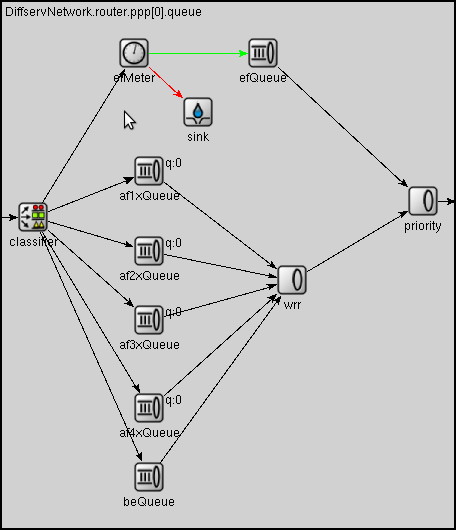
\includegraphics[scale=0.7]{figures/DiffservQueue.png}
\end{center}

The incoming packets are first classified according to
their DSCP field. DSCPs other than AFxy and EF are handled
as BE (best effort).

EF packets are stored in a dedicated queue, and served first
when a packet is requested. Because they can preempt the other
queues, the rate of the EF packets should be limited to a fraction
of the bandwith of the link. This is achieved by metering the EF
traffic with a token bucket meter and dropping packets that
does not conform to the traffic profile.

There are other queues for AFx classes and BE. The AFx queues
use RED to implement 3 different drop priorities within the class.
BE packets are stored in a drop tail queue.
Packets from AFxy and BE queues are sheduled by a WRR scheduler,
which ensures that the remaining bandwith is allocated among the classes
according to the specified weights.

%%% Local Variables:
%%% mode: latex
%%% TeX-master: "usman"
%%% End:



\cleardoublepage

\chapter{The MPLS Models}
\label{cha:mpls}

\section{Overview}
\label{sec:mpls:overview}

Multi-Protocol Label Switching (MPLS) is a ``layer 2.5'' protocol for
high-performance telecommunications networks. MPLS directs data from one network
node to the next based on numeric labels instead of network addresses, avoiding
complex lookups in a routing table and allowing traffic engineering.
The labels identify virtual links (label-switched paths or LSPs, also
called MPLS tunnels) between distant nodes rather than endpoints. The routers
that make up a label-switched network are called label-switching routers (LSRs)
inside the network (``transit nodes''), and label edge routers (LER) on the
edges of the network (``ingress'' or ``egress'' nodes).

A fundamental MPLS concept is that two LSRs must agree on the meaning of the
labels used to forward traffic between and through them.
This common understanding is achieved by using signaling protocols by which one
LSR informs another of label bindings it has made. Such signaling protocols are
also called label distribution protocols. The two main label distribution
protocols used with MPLS are LDP and RSVP-TE.

INET provides basic support for building MPLS simulations. It provides models
for the MPLS, LDP and RSVP-TE protocols and their associated data structures,
and preassembled MPLS-capable router models.

\section{Core Modules}
\label{sec:mpls:core-modules}

The core modules are:

\begin{itemize}
  \item \nedtype{Mpls} implements the MPLS protocol
  \item \nedtype{LibTable} holds the LIB (Label Information Base)
  \item \nedtype{Ldp} implements the LDP signaling protocol for MPLS
  \item \nedtype{RsvpTe} implements the RSVP-TE signaling protocol for MPLS
  \item \nedtype{Ted} contains the Traffic Engineering Database
  \item \nedtype{LinkStateRouting} is a simple link-state routing protocol
  \item \nedtype{SimpleClassifier} is a configurable ingress classifier for MPLS
\end{itemize}

\subsection{Mpls}
\label{sec:mpls:mpls}

The \nedtype{Mpls} module implements the MPLS protocol. MPLS is situated between
layer 2 and 3, and its main function is to switch packets based on their labels.
For that, it relies on the data structure called LIB (Label Information Base).
LIB is fundamentally a table with the following columns: \textit{input-interface},
\textit{input-label}, \textit{output-interface}, \textit{label-operation(s)}.

Upon receiving a labelled packet from another LSR, MPLS first extracts the
incoming interface and incoming label pair, and then looks it up in local LIB.
If a matching entry is found, it applies the prescribed label operations, and
forwards the packet to the output interface.

Label operations can be the following:

\begin{itemize}
  \item \textit{Push} adds a new MPLS label to a packet. (A packet may
     contain multiple labels, acting as a stack.) When a normal IP packet
     enters an LSP, the new label will be the first label on the packet.
  \item \textit{Pop} removes the topmost MPLS label from a packet.
     This is typically done at either the penultimate or the egress router.
  \item \textit{Swap}: Replaces the topmost label with a new label.
\end{itemize}

In INET, the local LIB is stored in a \nedtype{LibTable} module in the router.

Upon receiving an unlabelled (e.g. plain IPv4) packet, MPLS first determines the
forwarding equivalence class (FEC) for the packet using an ingress classifier,
and then inserts one or more labels in the packet's newly created MPLS header.
The packet is then passed on to the next hop router for the LSP.

The ingress classifier is also a separate module; it is selected depending
on the choice of the signaling protocol.


\subsection{LibTable}
\label{sec:mpls:libtable}

\nedtype{LibTable} stores the LIB (Label Information Base), as described
in the previous section. \nedtype{LibTable} is expected to have one instance
in the router.

LIB is normally filled and maintained by label distribution protocols (RSVP-TE,
LDP), but in INET it is possible to preload it with initial contents.

The \nedtype{LibTable} module accepts an XML config file whose structure
follows the contents of the LIB table. An example configuration:

\begin{XML}
<libtable>
    <libentry>
        <inLabel>203</inLabel>
        <inInterface>ppp1</inInterface>
        <outInterface>ppp2</outInterface>
        <outLabel>
            <op code="pop"/>
            <op code="swap" value="200"/>
            <op code="push" value="300"/>
        </outLabel>
        <color>200</color>
    </libentry>
</libtable>
\end{XML}

There can be multiple \ttt{<libentry>} elements, each describing a row in the
table. Colums are given as child elements: \ttt{<inLabel>}, \ttt{<inInterface>},
etc. The \ttt{<color>} element is optional, and it only exists to be able to
color LSPs on the GUI. It is not used by the protocols.

\subsection{Ldp}
\label{sec:mpls:ldp}

The \nedtype{Ldp} module implements the Label Distribution Protocol (LDP).
LDP is used to establish LSPs in an MPLS network when traffic engineering is not
required. It establishes LSPs that follow the existing IP routing table, and is
particularly well suited for establishing a full mesh of LSPs between all of the
routers on the network.

LDP relies on the underlying routing information provided by a routing protocol
in order to forward label packets. The router's forwarding information base, or
FIB, is responsible for determining the hop-by-hop path through the network.

In INET, the \nedtype{Ldp} module takes routing information from \nedtype{Ted}
module. The \nedtype{Ted} instance in the network is filled and maintained
by a \nedtype{LinkStateRouting} module. Unfortunately, it is currently not
possible to use other routing protocol implementations such as \nedtype{Ospf}
in conjunction with \nedtype{Ldp}.

When \nedtype{Ldp} is used as signaling protocol, it also serves as ingress
classifier for \nedtype{Mpls}.

\subsection{Ted}
\label{sec:mpls:ted}

The \nedtype{Ted} module contains the Traffic Engineering Database (TED).
In INET, \nedtype{Ted} contains a link state database, including reservations
for each link by RSVP-TE.

\subsection{LinkStateRouting}
\label{sec:mpls:linkstaterouting}

The \nedtype{LinkStateRouting} module provides a simple link state routing
protocol. It uses \nedtype{Ted} as its link state database. Unfortunately, the
\nedtype{LinkStateRouting} module cannot operate independently, it can only be
used inside an MPLS router.

 \subsection{RsvpTe}
\label{sec:mpls:rsvpte}

The \nedtype{RsvpTe} module implements RSVP-TE (Resource Reservation Protocol --
Traffic Engineering), as signaling protocol for MPLS. RSVP-TE handles bandwidth
allocation and allows traffic engineering across an MPLS network. Like LDP, RSVP
uses discovery messages and advertisements to exchange LSP path information
between all hosts. However, whereas LDP is restricted to using the configured
IGP's shortest path as the transit path through the network, RSVP can take
taking into consideration network constraint parameters such as available
bandwidth and explicit hops. RSVP uses a combination of the Constrained Shortest
Path First (CSPF) algorithm and Explicit Route Objects (EROs) to determine how
traffic is routed through the network.

When \nedtype{RsvpTe} is used as signaling protocol, \nedtype{Mpls} needs a
separate ingress classifier module, which is usually a \nedtype{SimpleClassifier}.

The \nedtype{RsvpTe} module allows LSPs to be specified statically in an XML
config file. An example \ttt{traffic.xml} file:

\begin{XML}
<sessions>
    <session>
        <endpoint>host3</endpoint>
        <tunnel_id>1</tunnel_id>
        <paths>
            <path>
                <lspid>100</lspid>
                <bandwidth>100000</bandwidth>
                <route>
                    <node>10.1.1.1</node>
                    <lnode>10.1.2.1</lnode>
                    <node>10.1.4.1</node>
                    <node>10.1.5.1</node>
                </route>
                <permanent>true</permanent>
                <color>100</color>
            </path>
        </paths>
    </session>
</sessions>
\end{XML}

In the route, \ttt{<node>} stands for strict hop, and \ttt{<lnode>} for loose hop.

Paths can also be set up and torn down dynamically with \nedtype{ScenarioManager}
commands (see chapter \ref{cha:scenario-scripting}).
\nedtype{RsvpTe} understands the \ttt{<add-session>} and \ttt{<del-session>}
\nedtype{ScenarioManager} commands. The contents of the \ttt{<add-session>}
element can be the same as the \ttt{<session>} element for the \ttt{traffic.xml}
above. The \ttt{<del-command>} element syntax is also similar, but only
\ttt{<endpoint>}, \ttt{<tunnel\_id>} and \ttt{<lspid>} need to be specified.

The following is an example \ttt{scenario.xml} file:

\begin{XML}
<scenario>
    <at t="2">
        <add-session module="LSR1.rsvp">
            <endpoint>10.2.1.1</endpoint>
            <tunnel_id>1</tunnel_id>
            <paths>
                ...
            </paths>
        </add-session>
    </at>
    <at t="2.4">
        <del-session module="LSR1.rsvp">
            <endpoint>10.2.1.1</endpoint>
            <tunnel_id>1</tunnel_id>
            <paths>
                <path>
                    <lspid>100</lspid>
                </path>
            </paths>
        </del-session>
    </at>
</scenario>
\end{XML}

\section{Classifier}
\label{sec:mpls:classifier}

The \nedtype{RsvpClassifier} module implements an ingress classifier for
\nedtype{Mpls} when using \nedtype{RsvpTe} for signaling. The classifier can be
configured with an XML config file.

\begin{inifile}
**.classifier.config = xmldoc("fectable.xml");
\end{inifile}

An example \ttt{fectable.xml} file:

\begin{XML}
<fectable>
    <fecentry>
        <id>1</id>
        <destination>host5</destination>
        <source>host1</source>
        <tunnel_id>1</tunnel_id>
        <lspid>100</lspid>
    </fecentry>
</fectable>
\end{XML}
\section{MPLS-Enabled Router Models}
\label{sec:mpls:mpls-enabled-router-models}

INET provides the following pre-assembled MPLS routers:

\begin{itemize}
  \item \nedtype{LdpMplsRouter} is an MPLS router with the LDP signaling protocol
  \item \nedtype{RsvpMplsRouter} is an MPLS router with the RSVP-TE signaling protocol
\end{itemize}

% HINT: A good MPLS primer:
% "MPLS for Dummies", Richard A Steenbergen <ras@nlayer.net>, nLayer Communications, Inc.
% https:www.nanog.org/meetings/nanog49/presentations/Sunday/mpls-nanog49.pdf


%%% Local Variables:
%%% mode: latex
%%% TeX-master: "usman"
%%% End:

\cleardoublepage

\chapter{Applications}
\label{cha:apps}


\section{Overview}

This chapter describes application models and traffic generators.

\section{TCP applications}

This sections describes the applications using the TCP protocol.
Each application must implement the \nedtype{ITCPApp} module interface
to ease configuring the \nedtype{StandardHost} module.

The applications described here are all contained by the
\nedtype{inet.applications.tcpapp} package. These applications use
\msgtype{GenericAppMsg} objects to represent the data sent between the client
and server. The client message contains the expected reply length, the
processing delay, and a flag indicating that the connection should be closed
after sending the reply. This way intelligence (behaviour specific to the
modelled application, e.g. HTTP, SMB, database protocol) needs only to be
present in the client, and the server model can be kept simple and dumb.


\subsection{TcpBasicClientApp}

Client for a generic request-response style protocol over TCP.
May be used as a rough model of HTTP or FTP users.

The model communicates with the server in sessions. During a session,
the client opens a single TCP connection to the server, sends several
requests (always waiting for the complete reply to arrive before
sending a new request), and closes the connection.

The server app should be \nedtype{TcpGenericServerApp}; the model sends
\msgtype{GenericAppMsg} messages.

Example settings:

FTP:

\begin{inifile}
numRequestsPerSession = exponential(3)
requestLength = truncnormal(20,5)
replyLength = exponential(1000000)
\end{inifile}

HTTP:

\begin{inifile}
numRequestsPerSession = 1 # HTTP 1.0
numRequestsPerSession = exponential(5)  # HTTP 1.1, with keepalive
requestLength = truncnormal(350,20)
replyLength = exponential(2000)
\end{inifile}

Note that since most web pages contain images and may contain frames,
applets etc, possibly from various servers, and browsers usually download
these items in parallel to the main HTML document, this module cannot
serve as a realistic web client.

Also, with HTTP 1.0 it is the server that closes the connection after
sending the response, while in this model it is the client.

\subsection{TcpSinkApp}

Accepts any number of incoming TCP connections, and discards whatever
arrives on them.

The module parameter \fpar{dataTransferMode} should be set the transfer mode in TCP layer.
Its possible values (``bytecount'', ``object'', ``bytestream'') are described in ...

\subsection{TcpGenericServerApp}

Generic server application for modelling TCP-based request-reply style
protocols or applications.

Requires message object preserving sendQueue/receiveQueue classes
to be used with \nedtype{Tcp} (that is, TCPMsgBasedSendQueue and TCPMsgBasedRcvQueue;
TCPVirtualBytesSendQueue/RcvQueue are not good).

The module accepts any number of incoming TCP connections, and expects
to receive messages of class \msgtype{GenericAppMsg} on them. A message should
contain how large the reply should be (number of bytes). \nedtype{TcpGenericServerApp}
will just change the length of the received message accordingly, and send
back the same message object. The reply can be delayed by a constant time
(replyDelay parameter).

\subsection{TcpEchoApp}

The \nedtype{TcpEchoApp} application accepts any number of incoming TCP
connections, and sends back the messages that arrive on them, The lengths of the
messages are multiplied by \fpar{echoFactor} before sending them back (echoFactor=1
will result in sending back the same message unmodified.) The reply can also be
delayed by a constant time (\fpar{echoDelay} parameter).

When \nedtype{TcpEchoApp} receives data packets from TCP (and such, when they can be
echoed) depends on the dataTransferMode setting.
With "bytecount" and "bytestream", TCP passes up data to us
as soon as a segment arrives, so it can be echoed immediately.
With "object" mode, our local TCP reproduces the same
messages that the sender app passed down to its TCP -- so if the sender
app sent a single 100 MB message, it will be echoed only when all
100 megabytes have arrived.

\subsection{TcpSessionApp}

Single-connection TCP application: it opens a connection, sends
the given number of bytes, and closes. Sending may be one-off,
or may be controlled by a "script" which is a series of
(time, number of bytes) pairs. May act either as client or as server,
and works with TCPVirtualBytesSendQueue/RcvQueue as sendQueue/receiveQueue
setting for ~TCP.
Compatible with both IPv4 (~IPv4) and ~IPv6.

\subsubsection*{Opening the connection}

Regarding the type of opening the connection, the application may
be either a client or a server. When active=false, the application
will listen on the given local localPort, and wait for an incoming connection.
When active=true, the application will bind to given local localAddress:localPort,
and connect to the connectAddress:connectPort. To use an ephemeral port
as local port, set the localPort parameter to -1.

Even when in server mode (active=false), the application will only
serve one incoming connection. Further connect attempts will be
refused by TCP (it will send RST) for lack of LISTENing connections.

The time of opening the connection is in the tOpen parameter.

\subsubsection*{Sending data}

Regardless of the type of OPEN, the application can be made to send
data. One way of specifying sending is via the tSend, sendBytes
parameters, the other way is sendScript. With the former, sendBytes
bytes will be sent at tSend. With sendScript, the format is
"<time> <numBytes>;<time> <numBytes>;..."

\subsubsection*{Closing the connection}

The application will issue a TCP CLOSE at time tClose. If tClose=-1, no
CLOSE will be issued.



\subsection{TelnetApp}

Models Telnet sessions with a specific user behaviour.
The server app should be \nedtype{TcpGenericServerApp}.

In this model the client repeats the following activity
between \fpar{startTime} and \fpar{stopTime}:

\begin{enumerate}
\item opens a telnet connection
\item sends \fpar{numCommands} commands. The command is \fpar{commandLength} bytes
      long. The command is transmitted as entered by the user character by character,
      there is \fpar{keyPressDelay} time between the characters. The server echoes
      each character. When the last character of the command is sent (new line),
      the server responds with a \fpar{commandOutputLength} bytes long message.
      The user waits \fpar{thinkTime} interval between the commands.
\item closes the connection and waits \fpar{idleInterval} seconds
\item if the connection is broken it is noticed after \fpar{reconnectInterval}
      and the connection is reopened
\end{enumerate}

Each parameter in the above description is ``volatile'', so you can
use distributions to emulate random behaviour.

Additional parameters:
addresses,ports
dataTransferMode

\begin{note}
This module emulates a very specific user behaviour, and as such,
it should be viewed as an example rather than a generic Telnet model.
If you want to model realistic Telnet traffic, you are encouraged
to gather statistics from packet traces on a real network, and
write your model accordingly.
\end{note}

\subsection{TcpServerHostApp}

This module hosts TCP-based server applications. It dynamically creates
and launches a new "thread" object for each incoming connection.

Server threads should be subclassed from the \cppclass{TcpServerThreadBase}
C++ class, registered in the C++ code using the Register\_Class() macro,
and the class name should be specified in the serverThreadClass
parameter of \nedtype{TcpServerHostApp}. The thread object will receive events
via a callback interface (methods like established(), dataArrived(),
peerClosed(), timerExpired()), and can send packets via TCPSocket's send()
method.

Example server thread class: \cppclass{TcpGenericServerThread}.

\begin{important}
Before you try to use this module, make sure you actually need it!
In most cases, \nedtype{TcpGenericServerApp} and \msgtype{GenericAppMsg} will be completely
enough, and they are a lot easier to handle. You'll want to subclass your
client from \cppclass{TCPGenericCliAppBase} then; check \nedtype{TelnetApp} and
\nedtype{TcpBasicClientApp} for examples.
\end{important}


\section{UDP applications}

All UDP applications should be derived from the \nedtype{IUDPApp} module interface,
so that the application of \nedtype{StandardHost} could be configured without changing its NED file.

The following applications are implemented in INET:
\begin{itemize}
\item \nedtype{UdpBasicApp} sends UDP packets to a given IP address at a given interval
\item \nedtype{UdpBasicBurst} sends UDP packets to the given IP address(es) in bursts, or acts as a packet sink.
\item \nedtype{UdpEchoApp} similar to \nedtype{UdpBasicApp}, but it sends back the packet after reception
\item \nedtype{UdpSink} consumes and prints packets received from the \nedtype{Udp} module
\item \nedtype{UdpVideoStreamClient},\nedtype{UdpVideoStreamServer} simulates UDP streaming
\end{itemize}

The next sections describe these applications in details.

\subsection{UdpBasicApp}

The \nedtype{UdpBasicApp} sends UDP packets to a the IP addresses given in the
\fpar{destAddresses} parameter. The application sends a message to one of the
targets in each \fpar{sendInterval} interval. The interval between message and
the message length can be given as a random variable. Before the packet is
sent, it is emitted in the \fsignal{sentPk} signal.

The application simply prints the received UDP datagrams. The \fsignal{rcvdPk}
signal can be used to detect the received packets.

The number of sent and received messages are saved as scalars at the end of the
simulation.

% could be a simple packet generator without the ability to receive packets?

\subsection{UdpSink}

This module binds an UDP socket to a given local port, and prints the
source and destination and the length of each received packet.

% TODO does not accept broadcast messages

\subsection{UdpEchoApp}

Similar to \nedtype{UdpBasicApp}, but it sends back the packet after reception.
It accepts only packets with \msgtype{UDPEchoAppMsg} type, i.e. packets that
are generated by another \nedtype{UdpEchoApp}.

When an echo response received, it emits an \fsignal{roundTripTime} signal.

\subsection{UdpVideoStreamClient}

This module is a video streaming client. It send one ``video streaming request'' to
the server at time \fpar{startTime} and receives stream from \nedtype{UdpVideoStreamServer}.

The received packets are emitted by the \fsignal{rcvdPk} signal.

\subsection{UdpVideoStreamServer}

This is the video stream server to be used with \nedtype{UdpVideoStreamClient}.

The server will wait for incoming "video streaming requests".
When a request arrives, it draws a random video stream size
using the \fpar{videoSize} parameter, and starts streaming to the client.
During streaming, it will send UDP packets of size \fpar{packetLen} at every
\fpar{sendInterval}, until \fpar{videoSize} is reached. The parameters \fpar{packetLen}
and \fpar{sendInterval} can be set to constant values to create CBR traffic,
or to random values (e.g. sendInterval=uniform(1e-6, 1.01e-6)) to
accomodate jitter.

The server can serve several clients, and several streams per client.

% FIXME why streamVector? VideoStreamData could be deleted immediately after last byte sent
% TODO this is video-on-demand, support multicast/broadcast video streaming too

\subsection{UdpBasicBurst}

Sends UDP packets to the given IP address(es) in bursts, or acts as a
packet sink. Compatible with both IPv4 and IPv6.

\subsubsection*{Addressing}

The \fpar{destAddresses} parameter can contain zero, one or more destination
addresses, separated by spaces. If there is no destination address given,
the module will act as packet sink. If there are more than one addresses,
one of them is randomly chosen, either for the whole simulation run,
or for each burst, or for each packet, depending on the value of the
\fpar{chooseDestAddrMode} parameter. The \fpar{destAddrRNG} parameter controls which
(local) RNG is used for randomized address selection.
The own addresses will be ignored.

An address may be given in the dotted decimal notation, or with the module
name. (The \cppclass{L3AddressResolver} class is used to resolve the address.)
You can use the "Broadcast" string as address for sending broadcast messages.

INET also defines several NED functions that can be useful:
\begin{itemize}
\item[-] moduleListByPath("pattern",...): \\
         Returns a space-separated list of the modulenames.
         All modules whole getFullPath() matches one of the pattern parameters will get included.
         The patterns may contain wilcards in the same syntax as in ini files.
         See cTopology::extractByModulePath() function
         example: destaddresses = moduleListByPath("**.host[*]", "**.fixhost[*]")
\item[-] moduleListByNedType("fully.qualified.ned.type",...): \\
         Returns a space-separated list of the modulenames with the given NED type(s).
         All modules whose getNedTypeName() is listed in the given parameters will get included.
         The NED type name is fully qualified.
         See cTopology::extractByNedTypeName() function
         example: destaddresses = moduleListByNedType("inet.nodes.inet.StandardHost")
\end{itemize}

The peer can be UDPSink or another UDPBasicBurst.

\subsubsection*{Bursts}

The first burst starts at \fpar{startTime}. Bursts start by immediately sending
a packet; subsequent packets are sent at \fpar{sendInterval} intervals. The
sendInterval parameter can be a random value, e.g. exponential(10ms).
A constant interval with jitter can be specified as 1s+uniform(-0.01s,0.01s)
or uniform(0.99s,1.01s). The length of the burst is controlled by the
\fpar{burstDuration} parameter. (Note that if \fpar{sendInterval} is greater than
\fpar{burstDuration}, the burst will consist of one packet only.) The time between
burst is the \fpar{sleepDuration} parameter; this can be zero (zero is not
allowed for \fpar{sendInterval}.) The zero \fpar{burstDuration} is interpreted as infinity.

\subsubsection*{Packets}

Packet length is controlled by the \fpar{messageLength} parameter.

The module adds two parameters to packets before sending:
\begin{itemize}
\item[-] sourceID: source module ID
\item[-] msgId: incremented by 1 after send any packet.
\end{itemize}
When received packet has this parameters, the module checks the order of received packets.

\subsubsection*{Operation as sink}

When \fpar{destAddresses} parameter is empty, the module receives packets and makes statistics only.

\subsubsection*{Statistics}

Statistics are collected on outgoing packets:
\begin{itemize}
\item[-] sentPk: packet object
\end{itemize}

Statistics are collected on incoming packets:
\begin{itemize}
\item[-] outOfOrderPk: statistics of out of order packets.
       The packet is out of order, when has msgId and sourceId parameters and module
       received bigger msgId from same sourceID.
\item[-] dropPk: statistics of dropped packets.
       The packet is dropped when not out-of-order packet and delay time is larger than
       delayLimit parameter. The delayLimit=0 is infinity.
\item[-] rcvdPk: statistics of not dropped, not out-of-order packets.
\item[-] endToEndDelay: end to end delay statistics of not dropped, not out-of-order packets.
\end{itemize}


\section{IPv4/IPv6 traffic generators}

The applications described in this section use the services of the network
layer only, they do not need transport layer protocols.
They can be used with both IPv4 and IPv6.

\nedtype{IIPvXTraffixGenerator} (prototype) sends IP or IPv6 datagrams to the
given address at the given \fpar{sendInterval}.
The \fpar{sendInterval} parameter can be a constant or a random value (e.g. exponential(1)).
If the \fpar{destAddresses} parameter contains more than one address, one
of them is randomly for each packet. An address may be given in the
dotted decimal notation (or, for IPv6, in the usual notation with colons),
or with the module name. (The \cppclass{L3AddressResolver} class is used to resolve
the address.) To disable the model, set destAddresses to "".

The \nedtype{IpvxTrafGen} sends messages with length \fpar{packetLength}.
The sent packet is emitted in the \fsignal{sentPk} signal.
The length of the sent packets can be recorded as scalars and vectors.

The \nedtype{IpvxTrafSink} can be used as a receiver of the packets
generated by the traffic generator. This module emits the packet
in the \fsignal{rcvdPacket} signal and drops it. The \ttt{rcvdPkBytes}
and \ttt{endToEndDelay} statistics are generated from this signal.

The \nedtype{IpvxTrafGen} can also be the peer of the traffic generators;
it handles the received packets exactly like \nedtype{IpvxTrafSink}.

\section{The PingApp application}

The \nedtype{PingApp} application
generates ping requests and calculates the packet loss and round trip
parameters of the replies.

Start/stop time, sendInterval etc. can be specified via parameters. An address
may be given in the dotted decimal notation (or, for IPv6, in the usual
notation with colons), or with the module name.
(The \cppclass{L3AddressResolver} class is used to resolve the address.)
To disable send, specify empty destAddr.

Every ping request is sent out with a sequence number, and replies are
expected to arrive in the same order. Whenever there's a jump in the
in the received ping responses' sequence number (e.g. 1, 2, 3, 5), then
the missing pings (number 4 in this example) is counted as lost.
Then if it still arrives later (that is, a reply with a sequence number
smaller than the largest one received so far) it will be counted as
out-of-sequence arrival, and at the same time the number of losses is
decremented. (It is assumed that the packet arrived was counted earlier as a loss,
which is true if there are no duplicate packets.)

Uses \msgtype{PingPayload} as payload for the ICMP(v6) Echo Request/Reply packets.

\subsection*{Parameters}

\begin{itemize}
  \item \fpar{destAddr}: destination address
  \item \fpar{srcAddr}: source address (useful with multi-homing)
  \item \fpar{packetSize}: of ping payload, in bytes (default is 56)
  \item \fpar{sendInterval}: time to wait between pings (can be random, default is 1s)
  \item \fpar{hopLimit}: TTL or hopLimit for IP packets (default is 32)
  \item \fpar{count}: stop after \fpar{count} ping request, 0 means continuously
  \item \fpar{startTime}: send first ping request at \fpar{startTime}
  \item \fpar{stopTime}: time of finish sending, 0 means forever
  \item \fpar{printPing}: dump on stdout (default is \fkeyword{false})
\end{itemize}

\subsection*{Signals and Statistics}

\begin{itemize}
  \item \fsignal{rtt} value of the round trip time
  \item \fsignal{numLost} number of lost packets
  \item \fsignal{outOfOrderArrivals} number of packets arrived out-of-order
  \item \fsignal{pingTxSeq} sequence number of the sent ping request
  \item \fsignal{pingRxSeq} sequence number of the received ping response
\end{itemize}

% FIXME seqNo should be part of ICMPMessage


\section{Ethernet applications}

The \nedtype{inet.applications.ethernet} package contains modules
for a simple client-server application. The \nedtype{EtherAppClient} is a simple
traffic generator that peridically sends \msgtype{EtherAppReq} messages
whose length can be configured. destAddress, startTime,waitType, reqLength, respLength

The server component of the model (\nedtype{EtherAppServer}) responds with a
\msgtype{EtherAppResp} message of the requested length. If the response does
not fit into one ethernet frame, the client receives the data in multiple
chunks.

% FIXME reqLength>1500 causes an error in the LLC module
% FIXME numFrames field of EtherAppRes is not used
% FIXME server always sends 1497 byte chunks, it should depend on the framing (1497 is for LLC)
% FIXME if registerSAP is false (default), the and EtherLLC used, then the client won't receive messages (auto config?)
% FIXME Ieee802Nic -> EthernetInterface in the NED comment

Both applications have a \fpar{registerSAP} boolean parameter.
This parameter should be set to \ttt{true} if the application is connected
to the \nedtype{EtherLlc} module which requires registration of the SAP
before sending frames.

Both applications collects the following statistics: sentPkBytes, rcvdPkBytes,
endToEndDelay.

The client and server application works with any model that accepts
Ieee802Ctrl control info on the packets (e.g. the 802.11 model).
The applications should be connected directly to the \nedtype{EtherLlc}
or an EthernetInterface NIC module.

The model also contains a host component that groups the applications
and the LLC and MAC components together (\nedtype{EtherHost}). This node does
not contain higher layer protocols, it generates Ethernet traffic directly.
By default it is configured to use half duplex MAC (CSMA/CD).



%%% Local Variables:
%%% mode: latex
%%% TeX-master: "usman"
%%% End:


\cleardoublepage

\chapter{Appendix: Author's Guide}
\label{cha:authors-guide}


\section{Overview}
\label{sec:authorsguide:overview}

This chapter is intended for authors and contributors of this 
\textit{INET Developer's Guide}, and covers the guidelines for deciding
what type of content is appropriate for this \textit{Guide} and 
what is not.

The main guiding principle is to avoid redundancy and duplication
of information with other pieces of documentation, namely:

\begin{itemize}
  \item Standards documents (RFCs, IEEE specifications, etc.) that
    describe protocols that INET modules implement;
  \item \textit{INET User's Guide}, which is intended for users who
    are interested in assembling simulations using the components
    provided by INET;
  \item \textit{INET Framework Reference}, directly generated from 
    NED and MSG comments by OMNeT++ documentation generator;
  \item Showcases, tutorials and simulation examples (\ttt{showcases/},
    \ttt{tutorials/} and \ttt{examples/} folders in the INET project)
\end{itemize}

Why is duplication to be avoided? Multiple reasons:

\begin{itemize}
  \item It is a waste of our reader's time they have to skip information
     they have already seen elsewhere
  \item The text can easily get out of date as the INET Framework evolves
  \item It is extra effort for maintainers to keep all copies up to date  
\end{itemize}


\section{Guidelines}
\label{sec:authorsguide:guidelines}

\subsection{Do Not Repeat the Standard}
\label{sec:authorsguide:do-not-repeat-standard}

When describing a module that implements protocol X, do not go
into lengths explaining what protocol X does and how it works,
because that is appropriately (and usually, much better) explained 
in the specification or books on protocol X. It is OK to summarize
the protocol's goal and principles in a short paragraph though.

In particular, do not describe the \textit{format of the protocol messages}.
It surely looks nice and takes up a lot of space, but the same information
can probably be found in a myriad places all over the internet.

\subsection{Do Not Repeat NED Documentation}
\label{sec:authorsguide:do-not-repeat-neddoc}

Things like module parameters, gate names, emitted signals and collected 
statistics are appropriately and formally part of the NED definitions,
and there is no need to duplicate that information in this \textit{Guide}.

Detailed information on the module, such as \textit{usage details} and the 
list of \textit{implemented standards} should be covered in the module's 
NED documentation, not in this \textit{Guide}.

\subsection{Do Not Repeat C++ Documentation}
\label{sec:authorsguide:do-not-repeat-cpp}

Describing every minute detail of C++ classes, methods, arguments are
expected to be appropriately present in their \textit{doxygen}
documentation.

\subsection{What then?}
\label{sec:authorsguide:what-then}

Concentrate on giving a ``big picture'' of the implementation: what it is
generally capable of, how the parts fit together, how to use the provided APIs,
what were the main design decisions, etc. Give simple yet meaningful examples
and just enough information about the API that after a quick read, users can
``bootstrap'' into implementing their own protocols and applications. If they
have questions afterwards, they will/should refer to the C++ documentation.



\cleardoublepage

\bibliographystyle{alpha}
\bibliography{inet-developers-guide}


%% no need for the following since 'tocbibind' package
%% \phantomsection
%% \addcontentsline{toc}{chapter}{\indexname}
\printindex

\end{document}
